\chapter{Distribuciones de Probabilidad}\label{distprob}



\begin{tikzpicture}
	\fill [left color=red!50, right color=teal!50] (0,0) rectangle (6.5,.1);
	\fill [left color=teal!50, right color=green!50] (6.5,0) rectangle (11.5,.1);
	\end{tikzpicture}

\emph{Las distribuciones de probabilidad son idealizaciones matemáticas de las distribuciones estadísticas (frecuencias relativas).}

Si los valores que toma una variable real $x$ dependen del azar, se dice que $x$ es una \emph{variable aleatoria}, v.a. Por ejemplo, los valores que toma la variable x que representa la suma de puntos obtenidos al lanzar un dado, $\{2,3,\cdots,12\}$.



	\begin{figure}[H]
	\centering
	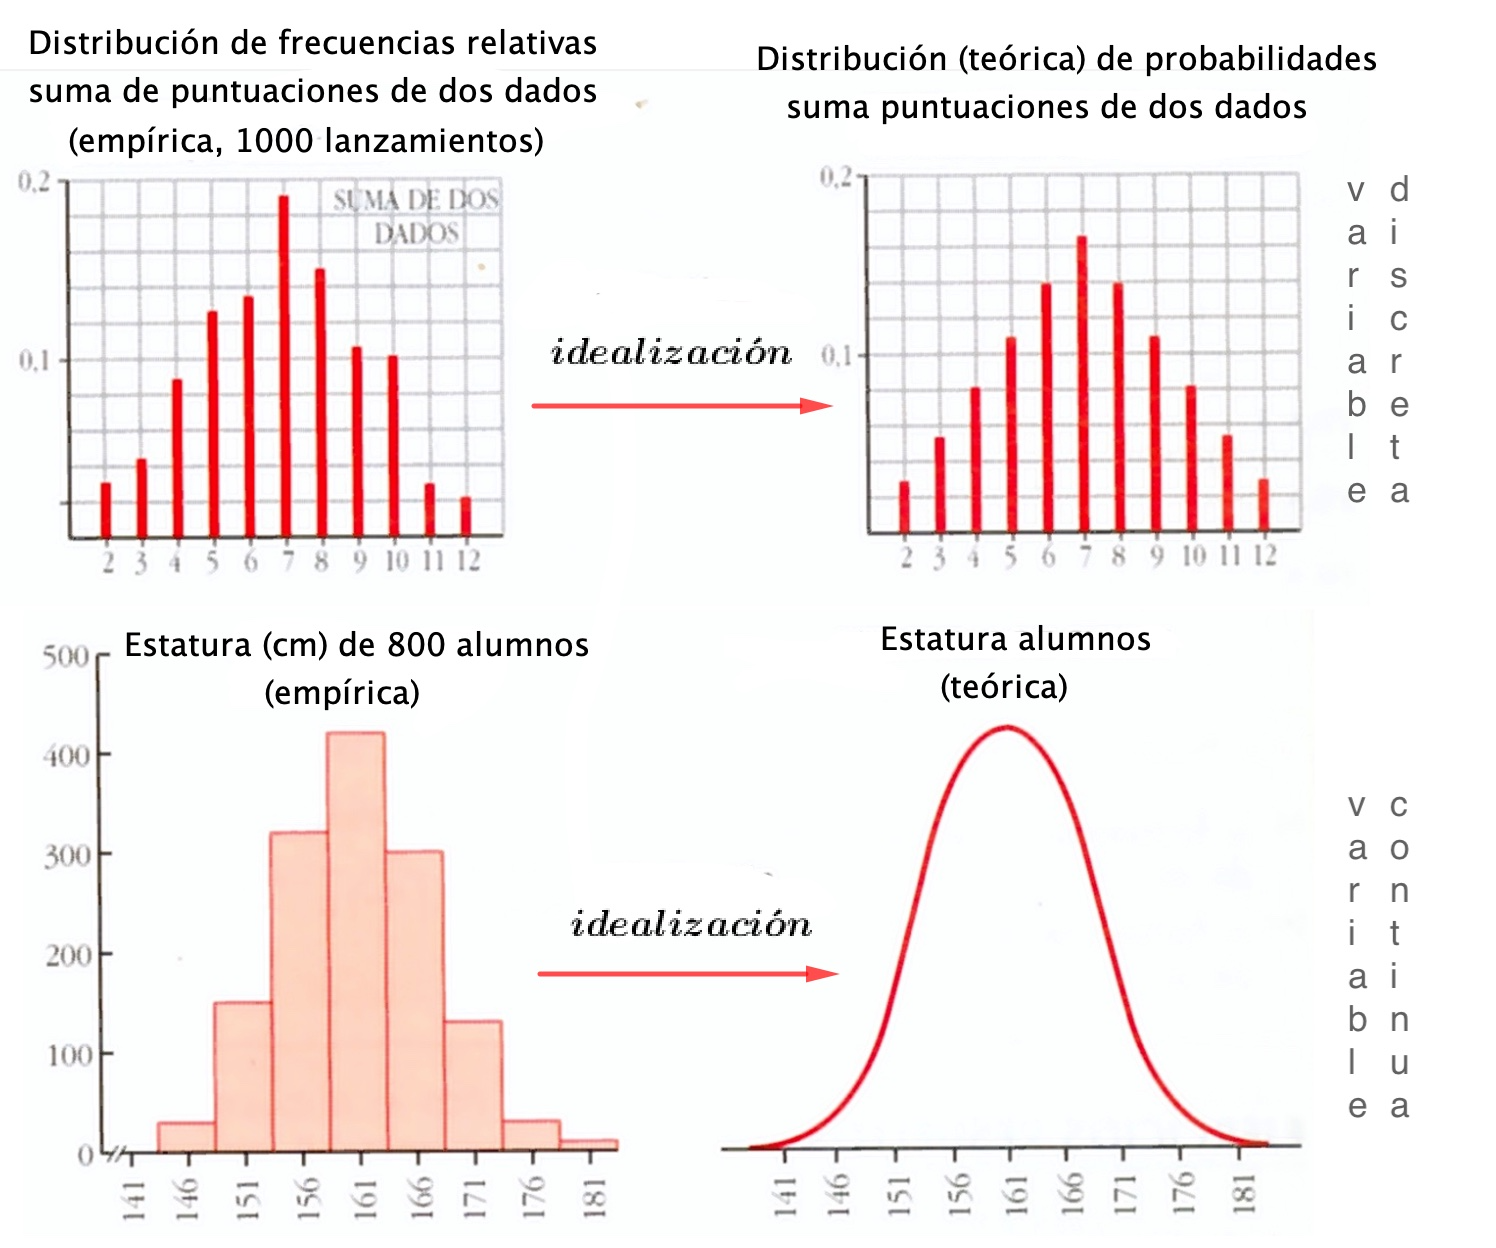
\includegraphics[width=.85\textwidth]{imagenes/imagenes04/T04IM01.png}
	\end{figure}


A cada valor $x_i$ le corresponderá un valor $p_i=p(x=x_i)$, probabilidad de que ocurra $x_i$. Diremos que los valores $(x_i, p_i)$ constituyen la \emph{distribución de probabilidad} de la v.a. x.

La distribución de probabilidad de una variable aleatoria es una función que asigna a cada suceso definido sobre la variable la probabilidad de que dicho suceso ocurra. La distribución de probabilidad está definida sobre el conjunto de todos los sucesos. Puede decirse que tiene una relación estrecha con las distribuciones de frecuencia. De hecho, una distribución de probabilidades no es más que una frecuencia teórica (modelo matemático, idealización).

La distribución de probabilidad queda determinada por la \emph{función de distribución}, cuyo valor en cada $x$ real es la probabilidad de que la variable aleatoria sea menor o igual que $x$.

\section{Variable aleatoria}

\begin{definition}
.	Sea $E$ el espacio muestral de un determinado experimento aleatorio. Se llama \textbf{variable aleatoria}, v.a., $X$, a toda aplicación
$\quad \boldsymbol{ X\ : \ E \ \to  \ \mathbb R }$

\vspace{2mm} Es decir, a la aplicación que asigna a cada suceso del espacio muestral un número real.

\begin{itemize}
\item Si el conjunto imagen, recorrido, $X(E)$ es finito, tenemos una \textbf{v.a. discreta}.	
\item Si el conjunto imagen, recorrido, $X(E)$ es un intervalo \textcolor{gris}{(que no sea un solo punto)}, tenemos una \textbf{v.a. continua}.
\end{itemize}
\end{definition}

\begin{example}
.	Consideremos el experimento aleatorio de lanzar dos dados.

\vspace{2mm} El espacio muestral es 	$E=\{(1,1); (1,2); (1,3) ; \cdots ; (1,6); (2,1); (2,2); \cdots ; (6,6) \}$

\vspace{2mm} Consideramos la v.a. $X$ tal que a cada elemento de $E$ le asocie su suma, es decir,

\vspace{2mm} $X(1,1)=2;\  X(1,2)=3; \  \cdots  ;\  X(2,2)=4;\  \cdots; \  X(6,6)=12$

\vspace{2mm} En este caso, $\quad X(E)=\{2,3,\cdots, 12\}$
\end{example}

\section{V.A. Discreta}

\subsection{Función de probabilidad}

\begin{definition}
.	$X$ es la v.a. discreta asociada al espacio muestral $E$, $x_i$ es un valor de la v. a. ($X=x_i\in X(E)$), la probabilidad de que ocurra $x_i$, de que la variable aleatoria $X$ tome el valor $x_i$ la denotamos por:
$P(X=x_i)=p_i$

\vspace{2mm} La aplicación: $\ P:\ X(E) \ \to \ \mathbb R \ : \ \ x_i \  \leadsto \ P(X=x_i)=P(x_i)=p_i\ $ 	  se llama \textbf{función de probabilidad o ley de probabilidad de la v.a. X}.
\end{definition}

\begin{example}
.	Considerando la v.a. del ejemplo anterior, y ayudándonos de una tabla de doble entrada donde representamos los 36 casos posibles en el lanzamiento de dos dados y la suma de sus puntuaciones, tenemos:	

\begin{multicols}{2}
% Please add the following required packages to your document preamble:
% \usepackage[table,xcdraw]{xcolor}
% If you use beamer only pass "xcolor=table" option, i.e. \documentclass[xcolor=table]{beamer}
\begin{table}[H]
\small
\centering
\begin{tabular}{c|c|c|c|c|c|c|}
 & {\color[HTML]{FE0000} \textbf{1}} & {\color[HTML]{FE0000} \textbf{2}} & {\color[HTML]{FE0000} \textbf{3}} & {\color[HTML]{FE0000} \textbf{4}} & {\color[HTML]{FE0000} \textbf{5}} & {\color[HTML]{FE0000} \textbf{6}} \\ \hline
{\color[HTML]{3531FF} \textbf{1}} & 2 & 3 & 4 & 5 & 6 & \underline{7} \\ \hline
{\color[HTML]{3531FF} \textbf{2}} & 3 & 4 & 5 & 6 & \underline{7} & 8 \\ \hline
{\color[HTML]{3531FF} \textbf{3}} & 4 & 5 & 6 & \underline{7} & 8 & 9 \\ \hline
{\color[HTML]{3531FF} \textbf{4}} & 5 & 6 & \underline{7} & 8 & 9 & 10 \\ \hline
{\color[HTML]{3531FF} \textbf{5}} & 6 & \underline{7} & 8 & 9 & 10 & 11 \\ \hline
{\color[HTML]{3531FF} \textbf{6}} & \underline{7} & 8 & 9 & 10 & 11 & 12 \\ \cline{2-7} 
\end{tabular}
\end{table}
	\begin{figure}[H]
			\centering
			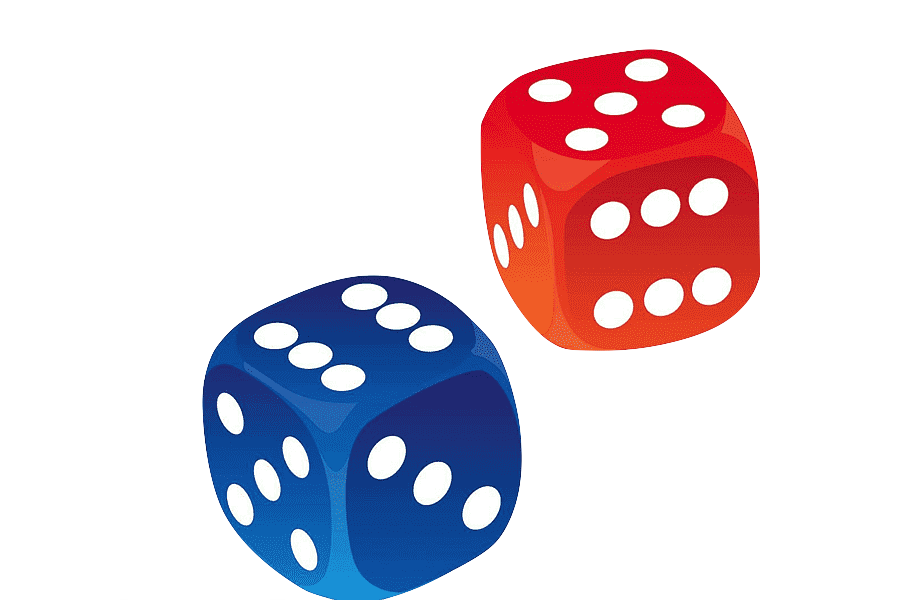
\includegraphics[width=.4\textwidth]{imagenes/imagenes02/T02IM15.png}
	\end{figure}
\end{multicols}

$P(X=2)=1/36=P(X=12);$ $P(X=3)=2/36=P(X=11);$ $P(X=4)=3/36=P(X=10);$ $P(X=5)=4/36=P(X=9);$ $P(X=6)=5/36=P(x=8);$ $P(X=7)=6/36$

\vspace{2mm} Nótese que $\ P(2)+P(3)+ \cdots + P(12)=36/36=1$

	\begin{figure}[H]
	\centering
	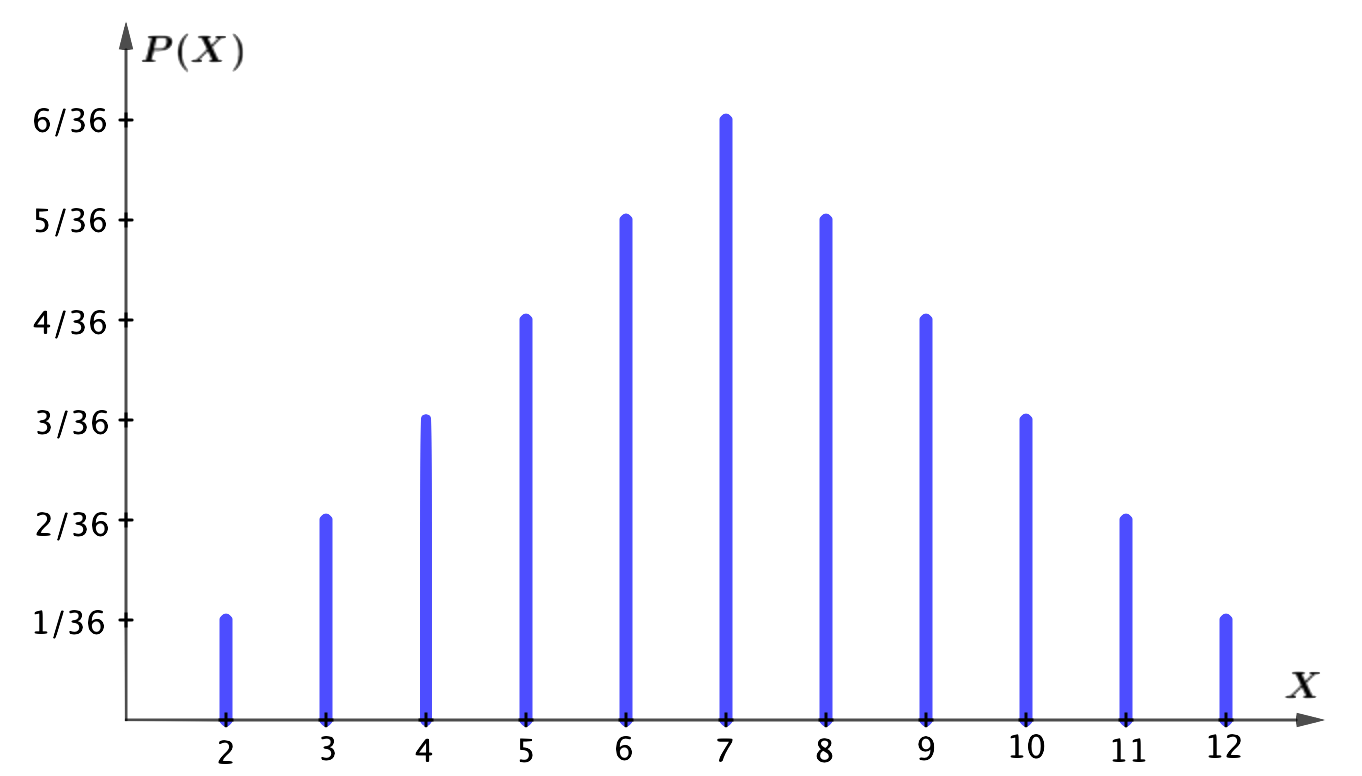
\includegraphics[width=.7\textwidth]{imagenes/imagenes04/T04IM03.png}
	\end{figure}
\end{example}

\subsection{Función de distribución}

\begin{definition}
.	Consideremos ordenada la v.a.: $\ X(E):\ x_1<x_2< \cdots <x_n$, la función: 

 $$F:\mathbb R \to \mathbb R \ / \ x \leadsto \boldsymbol{ F(x)=P(X\le x) }$$ 
 
 se llama \textbf{función de distribución} de la v.a. $X$ 	

\vspace{2mm} Si $x_k\le x\le x_{k+1} \ \to \ F(x)=P(x_1)+P(x_2)+ \cdots + P(x_k)$, es decir, $F(x)$ es la suma de las probabilidades de lo sucesos elementales $x_i$ tales que $x_i\le x$. 

\vspace{2mm} \emph{La función de distribución es el concepto idealizado de la frecuencia relativa acumulada de una distribución estadística}. $F$ es la `probabilidad acumulada'.
\end{definition}

\vspace{1cm}%********************************
\begin{theorem}
.	Propiedades de la función de distribución:

	 $1)\ F$ es creciente; 
	 $\qquad 2)\ F$ es escalonada;
	$\qquad 3)\ P[x_i < x \le x_j]\ = \ F(x_j)-F(x_i)$	
	
\end{theorem}


\vspace{1cm}%********************************
\begin{example}
.	La función de distribución de los ejemplos	anteriores es:

\vspace{2mm} \begin{small} \textcolor{gris}{$P(X=2)=1/36=P(X=12);$ $P(X=3)=2/36=P(X=11);$ $P(X=4)=3/36=P(X=10);$ $P(X=5)=4/36=P(X=9);$ $P(X=6)=5/36=P(x=8);$ $P(X=7)=6/36$} \end{small}

	\begin{figure}[H]
	\centering
	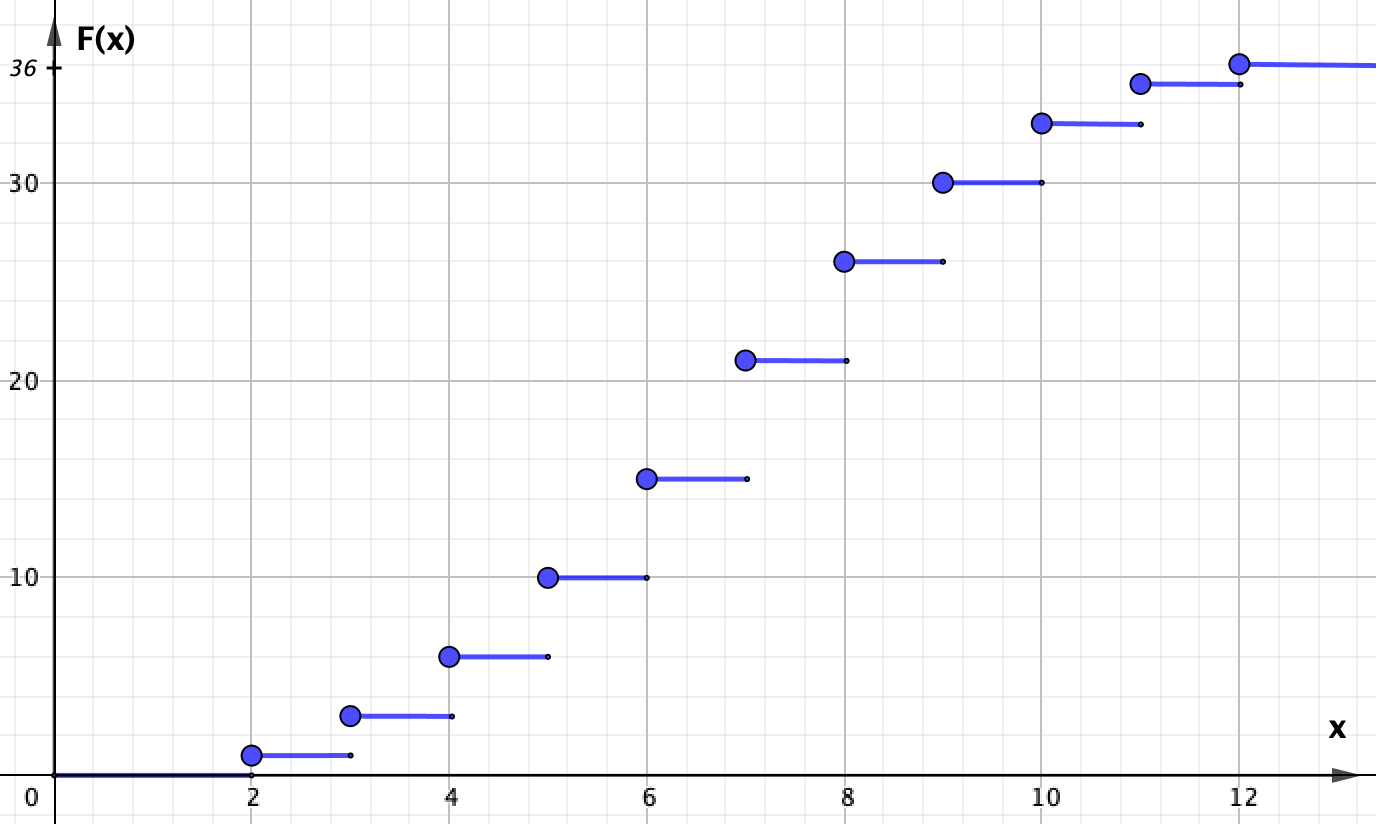
\includegraphics[width=.85\textwidth]{imagenes/imagenes04/T04IM04.png}
	\end{figure}
	
\end{example}


\vspace{1cm}%********************************
\subsection{Esperanza matemática, varianza y desviación típica}

% Please add the following required packages to your document preamble:
% \usepackage{multirow}
\begin{table}[H]
\centering
\begin{tabular}{cc|cccccc|ccccc}
\multirow{2}{*}{\begin{tabular}[c]{@{}c@{}}variable\\ estadística\\ discreta\end{tabular}} & $X$ & $x_1$ & $x_2$ & $\cdots$ & $x_n$ & $\ \ $ idealización $\ \ $  & $X$ & $x_1$ & $x_2$ & $\cdots$ & $x_n$ & \multirow{2}{*}{\begin{tabular}[c]{@{}c@{}}variable\\ aleatoria\\ diccreta\end{tabular}} \\ \cline{2-6} \cline{8-12}
 & $f$ & $f_1$ & $f_2$ & $\cdots$ & $f_n$ & $\quad \to \quad$ & $P$ & $p_1$ & $p_2$ & $\cdots$ & $p_n$ & 
\end{tabular}
\end{table}

\newpage %********************************************
\vspace{3mm} \begin{definition}
.	Al igual que la distribución estadística tenía $\bar x, \ s_x^2, \ s_x$, la \textbf{distribución de probabilidad} también tendrá \textbf{esperanza matemática, valor esperado o media}, que ahora denotaremos por $\boldsymbol \mu$, y \textbf{varianza y desviación típica}, $\boldsymbol{\sigma^2,\ \sigma}$

$\quad E(x)\ =\ \mu \ = \ x_1 P(x_1)+x_2 P(x_2)+ \cdots + x_n P(x_n)\ = \  \displaystyle \sum_{i=1}^n \ x_i \ P(x_i)$

$\quad  \sigma^2 \ = \  (x_1-\mu)^2 P(x_1)+ (x_2-\mu)^2 P(x_2) + \cdots + (x_n-\mu)^2 P(x_n) \ = \ \displaystyle \sum_{i=1}^n \ (x_i-\mu)^2 P(x_i) $

$\quad \sigma \ = \ \sqrt{\displaystyle \sum_{i=1}^n \ (x_i-\mu)^2 P(x_i)}$

\end{definition}

\vspace{2mm} \underline{Notación:} para distribuciones estadísticas: $\ \boldsymbol{ \bar x; \ s_x }$, en distribuciones de probabilidad $\ \boldsymbol{ \mu;\ \sigma}$

\vspace{2mm} \begin{theorem}
.	Propiedad: se cumple que

$$\sigma^2 \ =  \ 	\displaystyle \sum_{i=1}^n\ x_i^2\ P(x_i) \ - \ \mu^2$$
\end{theorem}

\begin{destacado}
	Si la v.a. X representa la ganancia o pérdida en un juego de azar, entonces la esperanza matemática representa la ganancia o pérdida media por jugada. Se dice que un \textbf{juego es justo} o equitativo si 	\textbf{la esperanza es cero}.
\end{destacado}


\begin{example}
	
Continuando con nuestro ejemplo de la suma de puntuaciones al lanzar dos dados,

\vspace{2mm} $\mu= 2\cdot 1/36 + 3 \cdot 2/36 + \cdots + 7 \cdot 6/36 + \cdots + 12\cdot 1/36= 7$

\vspace{2mm} Haciendo los cálculos necesarios, se obtiene: $\ \sigma^2=54.83;\quad \sigma=2.42$
\end{example}

\vspace{2mm} Alrededor de los 2/3 de las veces que se lance el dado se obtendrán puntuaciones comprendidas en $\mu \pm \sigma=7\pm 2.42 \approx (5,9)$, es decir, alrededor del 67\% de las veces, los dados sumarán 5, 6, 7, 8 o 9. (\emph{Interpretación conjunta de $\mu$ y $\sigma$}).


\vspace{4mm}
\begin{ejemplo}
	\begin{ejre}
	Considera la variable aleatoria X que describe las puntuaciones obtenidas la lanzar un dado.
	
	\vspace{2mm} Describe X y representa su función de probabilidad y su función de distribución. 
	
	\vspace{2mm} Calcula la esperanza matemática y la desviación típica de las puntuaciones obtenidas al lanzar un dado.
	
	\rule{100pt}{0.1pt}
	
	$X=\{1,2,3,4,5,6\}; \quad P(X=x_i)=p(x_i)=1/6,\ \forall i=\{1,\cdots, 6\}$. Todas las puntuaciones tienen la misma probabilidad, 1/6, de salir.
	
	\begin{figure}[H]
	\centering
	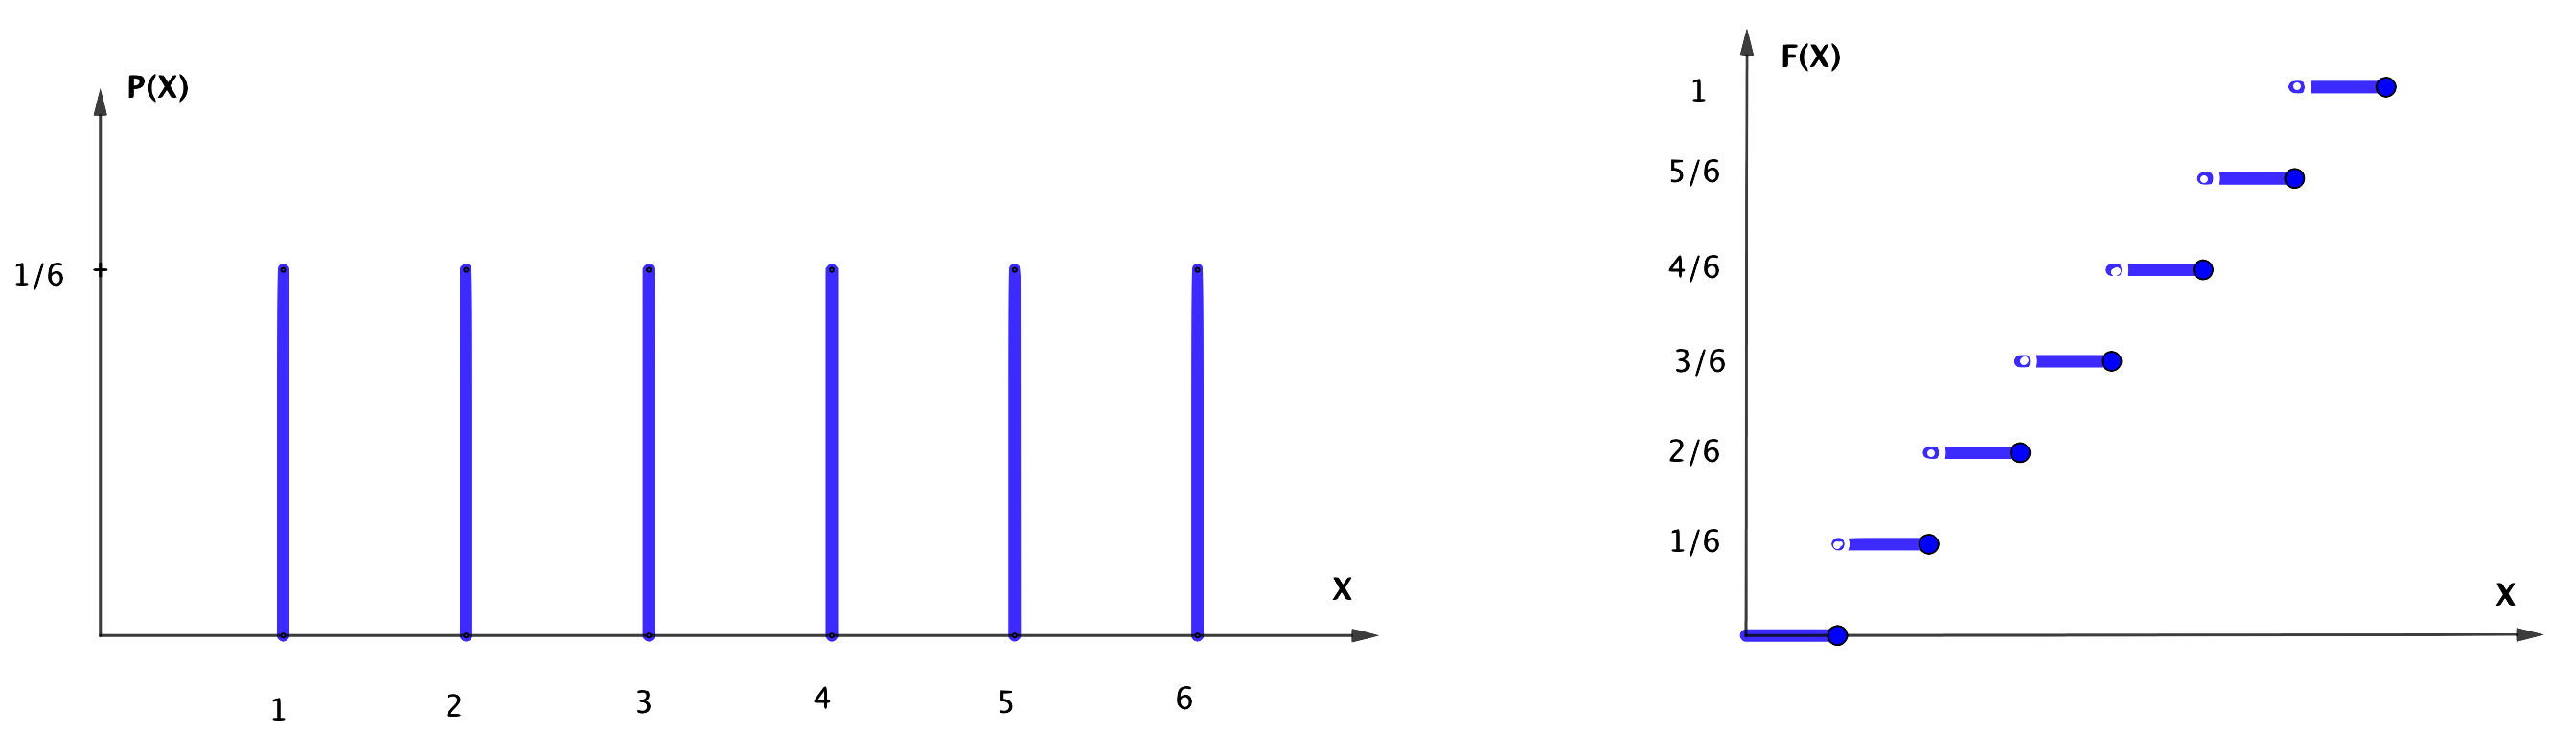
\includegraphics[width=.95\textwidth]{imagenes/imagenes04/T04IM06.png}
	\end{figure}
	
	\begin{multicols}{2}
	\begin{table}[H]
	\small
	\centering
	\begin{tabular}{r|rrrrrr}
	$\boldsymbol{x_i}$ & 1 & 2 & 3 & 4 & 5 & 6 \\ \hline
	$\boldsymbol{p_i}$ & 1/6 & 1/6 & 1/6 & 1/6 & 1/6 & 1/6
	\end{tabular}
	\end{table}

	$\qquad$ Haciendo los cálculos: 
	
	$\qquad \mu=3.5;\quad \sigma=3.9$
	\end{multicols}
	\end{ejre}
\end{ejemplo}

\vspace{1cm}%******************************
\begin{example}
.	Es costumbre penalizar los errores en exámenes tipo test	, lo cual es obvio para que ningún estudiante opte a tener un determinado número de aciertos si contesta al azar. En el caso de exámenes de preguntas con tres respuestas, cada acierto se contrarresta con dos fallos. Veamos por qué.

\vspace{2mm} Cuando se responda al azar, la puntuación debería ser cero. Esta debería ser su calificación esperada, su esperanza matemática.

\vspace{2mm} En este caso, al contestar al azar,  $p(acierto)=1/3;\ p(fallo)=2/3$. Si otorgamos $1$ punto por cada acierto, deberemos penalizar (restar) con $x$ puntos por cada fallo con objeto de que la esperanza matemática de su calificación sea cero:

\vspace{2mm} $\mu= E(X)=1\cdot \frac 1 3 + x \cdot \frac 2 3 =0 \ \to \ x=- \frac 1 2$, por cada error restaremos $0.5$ puntos (un acierto se compensa con dos fallos).
\end{example}


\section{Distribución binomial}


Distribuciones de probabilidad de v.a. discreta (idealizaciones o modelos matemáticos que representen distribuciones estadísticas) hay muchísimas. La más importante y famosa de ellas es la \emph{distribución binomial}, pero veamos unas más sencillas:

\vspace{15mm}  %*****************************************

\textbf{\large{Distribución uniforme}} \normalsize{(discreta)}.

\begin{definition}
.	Sea $X$ una v.a. discreta que toma los valores $\{x_1,x_2,\cdots ,x_n\}$ donde la probabilidad de tomar cualquiera de ellos es la misma en todos los casos: $p(X=x_i)=\frac 1 n,\ \forall i$.

$X$ se distribuye como una v.a. discreta \textbf{uniforme}, es la distribución más sencilla.


\vspace{2mm}  Se cumple que: $\displaystyle {E}[X]=\mu=\frac{1}{n} \sum_{i=1}^{n} x_{i};\quad {Var}(X)= \frac{1}{n} \sum_{i=1}^n(x_i - {E}[X])^2$
\end{definition}


\vspace{2mm}\textcolor{gris}{Si la v.a. discreta toma los valores $1,2,\cdots, n$ con probabilidades $p(x=i)=1/n,\ \forall i=1,2,\cdots , n$, se tiene que $\mu=(n+1)/2 \ \text{ y } \ \sigma^2=(n^2-1)/12$}


\vspace{2mm}  \underline{Ejemplo}: Resultados al lanzar un dado. (Ejercicio resuelto 4.1)


\vspace{15mm}  %*****************************************

\textbf{\large{Distribución de Bernouilli}}.

\normalsize{Un} experimento que sólo admite 2 resultados posibles excluyentes:

\hspace{1cm} --- Suceso A (representa el  éxito) con probabilidad $P (A) = p$.

\hspace{1cm} --- Suceso A' (representa el fracaso, contrario a A) con probabilidad $P(A') =1-p=q$,

recibe el nombre de \emph{prueba de Bernouilli}.

\begin{definition}
	.  \vspace{2mm}  Consideremos la v.a.discreta $X$ asociada al experimento que asocia el valor $1$ al suceso $A$, éxito,  con probabilidad $p$ y el valor $0$ al suceso $A'$, fracaso (0 éxitos), con probabilidad $q$. Esta variable recibe el nombre de \emph{variable de Bernouilli} y se denota por $X \leadsto Ber(p)$.

\vspace{2mm}  La distribución de probabilidad (función de probabilidad) es:
$\ P (X = 1) = p \text{ y } P (X = 0) = 1-p=q,  \text{ con } p+q= 1$
y su media, varianza y desviación típica son:
$\ \mu =p ,\  \sigma^2 =p\cdot q ,\  \sigma =\sqrt{p\cdot q}$
\end{definition}



\vspace{2mm} \underline{Ejemplos}: Estudiar los resultados de lanzar una moneda perfecta o trucada, el sexo de una persona, el que una determinada pieza fabricada sea defectuosa, etc. Todos ellos corresponden a experimentos con dos resultados posibles e incompatibles y no necesariamente de igual probabilidad, son distribuciones de Bernouilli.


%\vspace{10mm}  %*****************************************

\textbf{\Large{\subrayado{\text{Distribución Binomial}}}}\normalsize{.}

\begin{definition}
.	Supongamos que se realizan $n$ pruebas de Bernouilli sucesivas e independientes. Entonces, a la variable aleatoria discreta
$X =$ ``número de veces que ocurre el suceso $A$ (éxito) en las $n$ pruebas''
se la denomina \textbf{variable binomial} de parámetros $n$ y $p$ y se denota por $X \leadsto B(n, p)$ donde $p$ es la probabilidad de  éxito en cada prueba de Bernouilli (ha de ser constante en todas las $n$ pruebas). 

\vspace{2mm} \textcolor{gris}{  La variable binomial $X$ se puede considerar como la suma de $n$ variables independientes de Bernouilli, es decir $X=X1+X2+...+Xn$ con $Xi \leadsto Ber(p)\quad \forall i=1,2,\cdots ,n$}

\vspace{2mm}  La v.a. definida toma los valores $\{0, 1, 2, ..., n\}$ con probabilidades:

$$P (X = k) \ = \mqty(n \\ k) \ p^k \ (1-p)^{n-k} \ = \   \mqty(n \\ k) \ p^k \ q^{n-k} ;\quad q=1-p; \quad k=0,1,2,\cdots ,n$$

y su media, varianza y desviación típica son:

$$ \mu = \ n \ p;\qquad \sigma^2 = n\ p \ q ; \qquad \sigma = \sqrt{n\ p\ q}$$

\textcolor{gris}{Los coeficientes de la binomial son números combinatorios $\quad \mqty(n\\ k)= \dfrac {n!}{k! (n-k)!}$}	

\rule{150pt}{0.1pt}

.	Distribución binomial:

\begin{itemize}
\item Consideramos un experimento aleatorio \emph{dicotómico}, es decir, solo consideramos dos posibilidades mutuamente excluyentes: se verifica el suceso $A$ al que llamamos \emph{éxito} o no se verifica, se verifica pues $A'$, contrario a $A$ y le llamamos \emph{fracaso}.
\item La probabilidad de que ocurra $A,\ p(A)=p=cte$ en el experimento y todas las veces que se realice la experiencia (las sucesivas \emph{pruebas son independientes} unas de otras). Por tanto, también la probabilidad de fracaso será constante, $p(A')=1-p(A)=1-p=q=cte$.
\item Realizamos el experimento $n$ veces y nos preguntamos por la probabilidad de tener $k$ éxitos. $k\in \{0,1,2,\cdots, n\}$. $X$ es la v.a. discreta binomial que describe el número de éxitos.	
\end{itemize}
	
	La \textbf{función de probabilidad de la v.a. binomial} es:
	
	$$\boldsymbol{f(X=k)\ =\ p(X=k)\ =\ \mqty(n\\k)\ p^k\ q^{n-k}}$$
	
	De aquí, la \textbf{función de distribución de la v.a. binomial} es:
	
	$$F(X=k)\ = \ \displaystyle \sum_{x_i\le k}\ \mqty(n\\ x_i) \ p^{x_i} \ q^{n-x_i} \qquad F(x<0)=0;\ \ F(x\ge n)=1$$
	
Como la distribución binomial de pende de dos parámetros, $n$ (número de experimentos) y $p$ (probabilidad de éxito), es costumbre hablar de ella en la forma $\ \boxed{\  \boldsymbol{B(n,p)} \ } \ $	
\end{definition}

\begin{comment}
% No acaba de quedar totalmente claro
Más concretamente, la función de distribución binomial es:

\begin{small}
$$F(x) \ = \ 
\begin{cases}
\ 0 & \text{si } x<0 \\
\ P(X\le x)=\mqty(n\\0)p^0q^n+\mqty(n\\1)p^1q^{n-1}+\cdots +\mqty(n\\x)p^xq^{n-x} & \text{si } 0\le x \le n \\
\ 1 & \text{si } n\ge x 	
 \end{cases}$$
\end{small}
\end{comment}

\begin{theorem}
.	Se demuestra que en una v.a. Binomial, $\ X\in B(n,p)$:

\vspace{4mm} \hspace{2cm} $\bold{\mu \ = E(X)\ = \ \ n \ p}$

\hspace{2cm} $\bold{\sigma^2 \ = \ n\ p \ q}$

\hspace{2cm} $\bold{\sigma\ = \ \sqrt{n\ p\ q}}$

\vspace{-5mm} \begin{center} \textcolor{gris}{\rule{75mm}{0.1mm}} \end{center}

\vspace{-5mm} $$P(X=x)=F(x)-F(x-1)$$

\end{theorem}

\begin{proof}
 Demostración del valor de la media en una $X\leadsto B(n,p):$ 	
 
 $\mu=E(X)=\displaystyle \sum_{x_0}^n\ x\ \mqty(n\\x)p^x(1-p)^{n-x}= 0 + 	\sum_{x_1}^n\ x\ \mqty(n\\x)p^x(1-p)^{n-x}= \sum_{x_1}^n\ x\ \mqty(n\\x)p^xq^{n-x}$
 
\begin{small}  Como $\ \mqty(n\\x)=\dfrac{n!}{x! \ (n-x)!}=\dfrac n x \dfrac{(n-1)!}{(x-1)!\ (n-x)!}= \dfrac n x \dfrac{(n-1)!}{(x-1)!\ [(n-1)-(x-1)]!}=\dfrac n x \mqty(n-1\\x-1)$ \end{small}

Luego, $\ E(X)=\displaystyle \sum_{x_1}^n \ \cancel{x} \dfrac {n}{\cancel{x}}
\mqty(n-1\\x-1) p^x q^{n-x}= n\ \sum_{x=1}^{n}\mqty(n-1\\x-1)p^xq^{n-x}$

Cambio: $ k\ = \ x-1 \to \begin{cases}
 \ x=1 \to k=0 \\ \ x=n \to k=n-1	
 \end{cases}$
 
 $E(X)=n \ \displaystyle \sum_{k=0}^{n-1} \mqty(n-1\\k)p^{k+1}q^{n-(k+1)}=
 np\ \sum_{k=0}^{n-1} \ \mqty(n-1\\k)p^kq^{(n-1)-k}$
 
 Binomio Newton: $\ (a+b)^n=\displaystyle \sum_{k=0}{n}\mqty(n\\k)a^kb^{n-k}$
 
 $\boldsymbol{ E(X)=\mu=} n\ p \ (p+1-p)^{n-1}= \boldsymbol{ n \ p}$

\end{proof}


\vspace{4mm} Son ejemplo de distribuciones binomiales:
número de caras al lanzar 100 monedas, número de hijas en 500 familias con 3 hijos,  número de familias con un solo hijo en una población de 1000 familias, número de accidentes de tráfico si han circulado 10000 automóviles, número de reacciones negativas ante un fármaco administrado a 5000 pacientes, etc

\vspace{4mm} \begin{example}
.	Se lanzan 6 dados, calcular la probabilidad de obtener exactamente dos cuatros.

\vspace{4mm} El experimento es similar a lanzar un dado 6 veces y observar cuantas veces sale 4.

\vspace{2mm} --- Tenemos una experiencia dicotómica, sale 4 (éxito) o no sale 4 al lanzar un dado. 	

--- La probabilidad de éxito es $p=1/6;\ q=1-p=5/6$ es la de fracaso. Estas probabilidades son constantes todas las veces que se lance el dado (veces que se realice la experiencia)

--- Realizamos el experimento $n=4$ veces y nos preguntamos por la probabilidad de que salgan dos cuatros $k=2$, tener 2 éxitos.

\vspace{2mm} Tenemos una $\boldsymbol{B(6,1/6)}$, luego, $f(2)=P(X=2)=\mqty(6\\2)(1/6)^2(5/6)^4=0.20$

\vspace{2mm} El valor esperado de éxitos (veces que sale el 4) en estos 6 experimentos es:
$\ E(X)=\mu=6\cdot 1/6=1$, por término medio saldrá un 4 de cada 6 lanzamientos, y la desviación típica es $\ \sigma=\sqrt{6\cdot 1/6\cdot 5/6}=0.91$
\end{example}

\begin{small}
\begin{adjustwidth}{20pt}{0pt}

\textcolor{gris}{\rule{75mm}{0.1mm}}

\textcolor{gris}{Sería conveniente repasar los ejercicios resueltos del tema 3 de probabilidad, 32, 33 y 34, así como el apéndice \ref{combinatoria} de combinatoria.}

\vspace{2mm}  \textcolor{gris}{Dos 4 en seis lanzamientos, ?`cuántos casos hay?. Representamos por $4$ el éxito y por $\_$ el fracaso, cuando sale cualquier número que no sea el cuatro.}

\vspace{2mm}\textcolor{gris}{$44\_\ \_\ \_\ \_; \ \_44\_\ \_\ \_; \ \ \_\ \_44\_ \ \_;\ \_\ \_\ \_44\_;\  \_\ \_\ \_\ \_ 44\quad $  Los 4 salen juntos.}


\textcolor{gris}{$4\_4\_\ \_\ \_;\ \_4\_4\_\ \_;\ \_\ \_4\_4\_;\ \_\ \_\ \_4\_4 \quad$ Les separa una posición.}

\textcolor{gris}{$4\_\ \_4\_\ \_;\ \_4\_\ \_4\_;\ \_\ \_\ \_4\_\ \_4 \quad$ Les separan dos posiciones.}

\textcolor{gris}{$4\_ \ \_\ \_4\_;\ \_4\_\ \_\ \_4 \quad$ Les separan tres posiciones.}

\textcolor{gris}{$4\_\ \_\ \_\ \_4 \quad$ Les separan cuatro posiciones.}

\vspace{2mm}\textcolor{gris}{En total tenemos $15$ formas distintas de obtener dos 4 (éxitos) en seis lanzamientos, $15=\mqty(6\\2)$. Todas ellas tienen la misma probabilidad:}

\vspace{2mm}\textcolor{gris}{$p(4\_\ \_\ \_4\_)=\frac 1 4 \ \frac 5 6 \ \frac 5 6 \ \frac 5 6 \ \frac 1 4 \ \frac 5 6 = \left( \frac 1 4 \right)^2\ \left( \frac 5 6 \right)^2$ $;\quad$ $p(44\_\ \_\ \_\ \_)=\frac 1 4 \ \frac 1 4 \ \frac 5 6 \ \frac 5 6 \ \frac 5 6 \ \frac 5 6 = \left( \frac 1 4 \right)^2\ \left( \frac 5 6 \right)^2$}

\vspace{2mm}\textcolor{gris}{En total, la probabilidad de obtener $x=2$ éxitos en los $n=6$ lanzamientos es:}

\vspace{2mm}\textcolor{gris}{$p(x=6)=\mqty(6\\2) \  (1/6)^2 \ (5/6)^4 = 15 \  (1/6)^2 \ (5/6)^4  =0.20$}

\vspace{-4mm}
\begin{flushright}
\textcolor{gris}{\rule{100mm}{0.1mm}}	
\end{flushright}

	
\end{adjustwidth}
\end{small}


\vspace{10mm} %****************************************** 

\begin{theorem}
.	\textbf{Propiedades de la distribución Binomial}:

\begin{enumerate}
	\item La distribución Binomial se puede obtener como suma de $n$ variables aleatoria independientes Bernouilli con el mismo parámetro $p$.
	\item Si tenemos dos variables aleatorias que se distribuyen según una Binomial con el mismo parámetro $p$, es decir, con la misma probabilidad de éxito, $X \to  B(n, p) \text{ e }  Y \to  B(m, p)$ , entonces siempre se verifica $X + Y \to  B(n + m, p)$. Si no tienen la misma probabilidad no se pueden sumar.
	\item Sea $X$ una variable aleatoria e $Y$ otra variable aleatoria que verifican que $X \to  B(n, p)$ e $Y=X/n$, entonces se verifica $Y \to  B(1, p / n)$ y además su esperanza y varianza son $E[Y]= p$ y $\sigma= pq/n$.	
\end{enumerate}
\end{theorem}


\vspace{10mm} %******************************************

\begin{ejemplo}
	\begin{ejre}
		En una celebración \textbf{muy numerosa} la gente se dispone en mesas de 5 comensales, hay tantas mujeres como hombres. En una de estas mesas, ?`cuál es la probabilidad de que hayan más mujeres que hombres? \textbf{?`Por qué decimos que la fiesta es muy numerosa?}
	\end{ejre}

\textcolor{gris}{\rule{75mm}{0.1mm}}

Solución:  $p(2^a\ chica)=\begin{cases}
\ p(2^a\ chica|1^a\ chica)=\dfrac{N/2-1}{N-1} \\
\ p(2^a\ chica|1^o\ chico)=\dfrac{N/2}{N-1}
\end{cases}$ Son distintas,
la diferencia es $\dfrac 1{N-1} \ \to 0 \ \ \text{ si } \ N>>1$ Es decir, si la fiesta es `muy numerosa', $N>>1$, entonces la probabilidad de elegir una chica de un grupo de $5$ es prácticamente constante y podemos considerar que tenemos una \emph{distribución binomial} $\boldsymbol{
B(5,1/2)}$, ya que hay tanto chico (fracaso) como chica (éxito), por lo que $p=q=1/2$.

\vspace{2mm} En un grupo de 5 personas (mesa), habrán más chicas si tenemos 3, 4 o 5 \emph{éxitos} en la $B(5,1/2)$, $\ F(3)=p(x\ge 3)=p(3)+p(4)+p(5)$

\vspace{2mm} $ p(3)=\mqty(5\\3)(1/2)^3\ (1/2)^2; \quad p(4)=\mqty(5\\4)(1/2)^4\ (1/2)^1; \quad p(3)=\mqty(5\\5)(1/2)^5\ (1/2)^0; \quad $

\vspace{2mm} Para calcular los coeficientes, número combinatorios, podemos acudir a la fila 5 del triángulo de Tartaglia (Ver \ref{tartaglia} ``números combinatorios'' en apéndice \ref{combinatoria} de combinatoria)

\begin{table}[H]
\centering
\begin{tabular}{ccccccccccc}
 &  &  &  & 1 &  & 1 &  &  &  &  \\
 &  &  & 1 &  & 2 &  & 1 &  &  &  \\
 &  & 1 &  & 3 &  & 3 &  & 1 &  &  \\
 & 1 &  & 4 &  & 6 &  & 4 &  & 1 &  \\
1 &  & 5 &  & 10 &  & \textbf{10} & \textbf{} & \textbf{5} & \textbf{} & \textbf{1} \\
 &  &  &  &  &  & \textcolor{gris}{$\mqty(5\\3)$} &  & \textcolor{gris}{$\mqty(5\\4)$} &  & \textcolor{gris}{$\mqty(5\\5)$}
\end{tabular}
\end{table}

$F(3)=p(x\ge 3)=[\ 10+5+1  \ ] \ (1/2)^5 \ = \ \dfrac{16}{2^5}\ = \ \dfrac 1 2 \ = \ 50\%$

\vspace{2mm} Además, el número esperado (media) de  chicas por mesa es, evidentemente,  
$E(X)=\mu=5\cdot \dfrac 1 2 = 2.5;\quad \text{con } \ \sigma=\sqrt{5\dfrac 1 2 \dfrac 1 2}=1.12$

\end{ejemplo}



\vspace{4mm} \begin{ejemplo}
	\begin{ejre}
		En una $B(10,0.8), \text{ calcular } F(X=9)=p(X\le 9)$
	\end{ejre}
\textcolor{gris}{\rule{75mm}{0.1mm}}

$F(X=9)=p(X\le 9)=p(8)+p(7)+\cdots +p(1)+p(0)=1-[ \ p(9)+p(10) \ ]$

En este caso, es más fácil (menos cálculos) pensar en el suceso contrario.

$F(x)=1-\mqty(10\\9)\ 0.8^9\ 0.2^1 - \mqty(10\\10)\ 0.8^{10}\ 0.2^0=0.597$

\end{ejemplo}

\begin{center} \textcolor{gris}{\rule{150mm}{0.1mm}} \end{center}

	\begin{figure}[H]
	\centering
	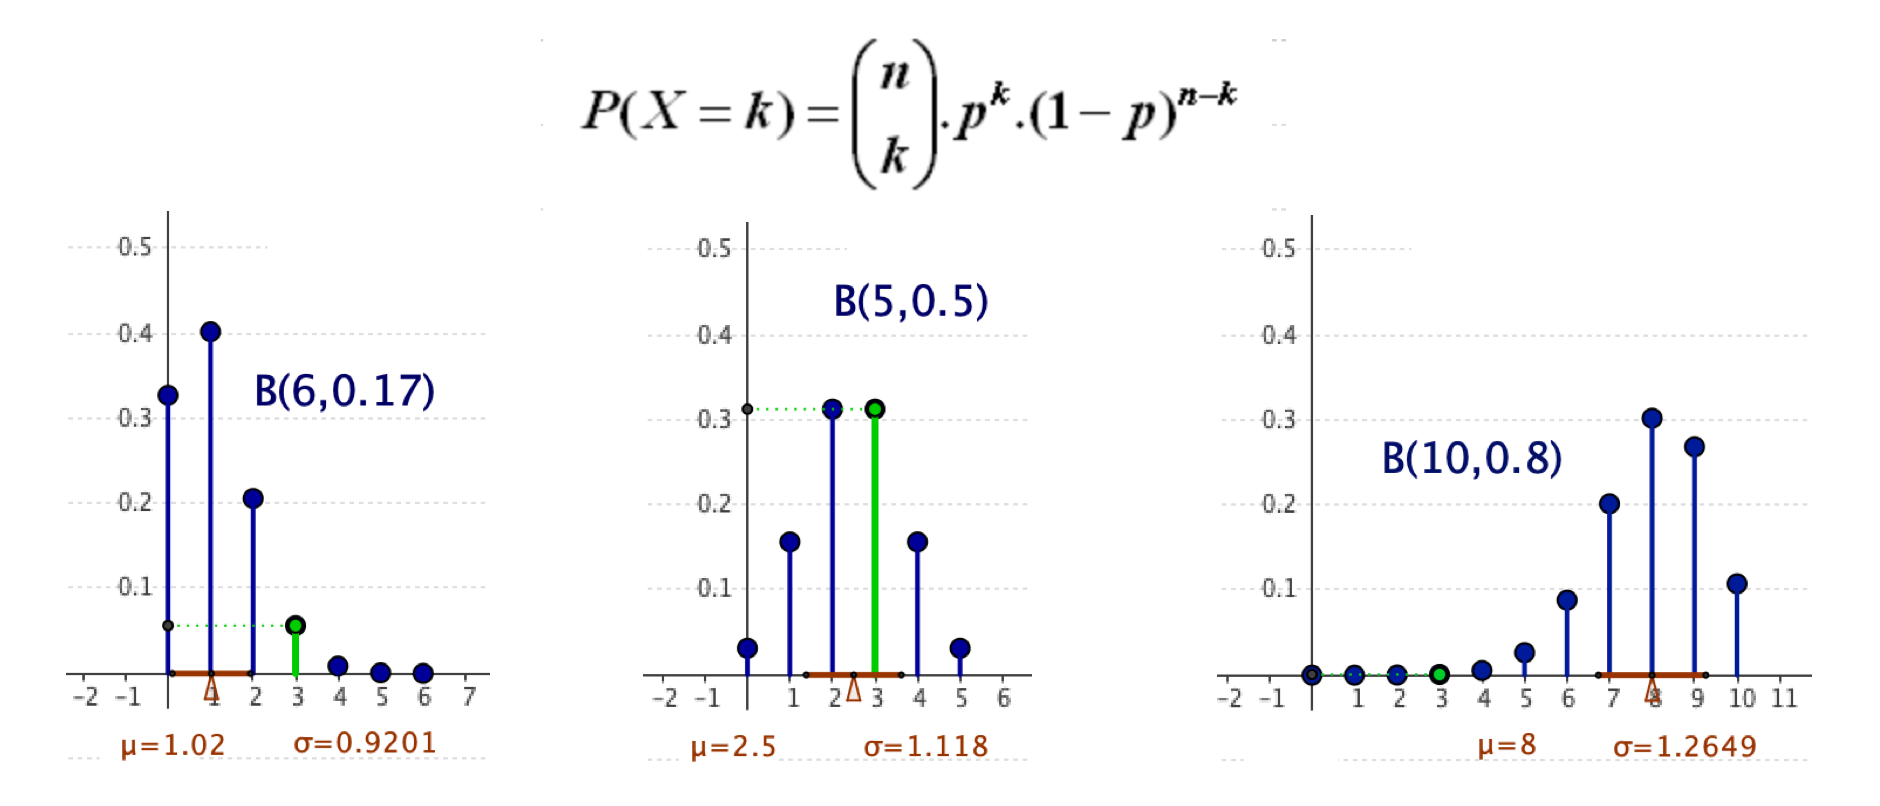
\includegraphics[width=1\textwidth]{imagenes/imagenes04/T04IM09.png}
	\end{figure}

Existen muchas más distribuciones de probabilidad de variable discreta, pero la binomial es la más importante. De todos modos, vamos a ver una distribución discreta más (también muy importante). Además, en determinadas condiciones (como veremos) sirve como aproximación de la binomial.

\vspace{10mm} 

\textbf{\large{Distribución de Poisson}}\normalsize{.}

\begin{definition}
.	Una variable aleatoria discreta X se dice que sigue una \textbf{distribución de Poisson} de parámetro $\lambda$ si X toma todos los valores 0, 1, 2, $\cdots$, n, con probabilidades en cada caso:

$$P(X=k)\ = \ \dfrac{\lambda^k}{k!}\ e^{-\lambda}$$	

Se denota por $\ X \ \leadsto \ P(\lambda) \ $ y se cumple que $\ E(X)=\mu=\lambda;\ \ \sigma=\sqrt{\lambda} \ $. 
\end{definition}

\vspace{4mm}La distribución de Poisson sirve para modelizar el número X de eventos que ocurren aleatoriamente en el tiempo o en una región. Algunos ejemplos de experimentos en los cuales la variable aleatoria puede ser modelizada con distribución de Poisson son:

--- El número de llamadas recibidas en una centralita durante un tiempo determinado.

--- El número de bacterias por volumen de fluido.

--- El número de llegadas de clientes a una caja de pago de un supermercado en un tiempo determinado. 

--- El número de piezas defectuosas que produce una máquina durante cierto día.

--- El número de accidentes de tránsito en un cruce dado durante un tiempo establecido.

--- El número de árboles de determinada especie distribuidos aleatoriamente en un  área de bosque.

Algunos de estos ejemplos son \emph{procesos temporales}, interesa conocer cuántas veces ocurre un evento en un intervalo de tiempo, y otros son \emph{procesos espaciales}, interesa conocer cuántos “puntos” hay en un volumen o un área.

\vspace{4mm}
\begin{definition}
.	Un proceso temporal de Poisson es cuando se cumplen con las siguientes características:

\vspace{2mm}
--- Invarianza: las condiciones no cambian en el tiempo.

--- Falta de memoria: lo que sucede en el intervalo de tiempo $[0, t_1)$ no influye en lo que suceda en el intervalo $[t_2, t_3)$, para $t_1<t_2<t_3$.

--- Sucesos aislados: la probabilidad de que en un intervalo de tiempo muy corto ocurra más de una vez el evento es despreciable comparada con la probabilidad de que ocurra una vez o ninguna.	

\vspace{4mm}

En estas condiciones, si $X_t$ es la v.a. que mide el número de veces que ocurre el evento en un intervalo de tiempo de longitud $t$, se demuestra que que $X_t$ es una variable aleatoria discreta cuya función de probabilidad viene dada por:

$$P(x)\ =\ \dfrac{(c\cdot t)^x}{x!}\ e^{-x};\quad x=0,1,2,\cdots $$

$X_t$ es una distribución de Poisson con parámetro $\lambda_t = c \cdot t$, con $c$  una constante positiva que indica la cantidad de veces que ocurre el evento de estudio por unidad de tiempo. $c$ se llama \emph{tasa de ocurrencia del proceso}.
\end{definition}

\vspace{4mm}
\begin{example}
.	Los clientes a un mostrador de un negocio se distribuyen con una distribución de Poisson a una tasa de 5 por hora. Si queremos saber cuál es la probabilidad de que no lleguen más de tres clientes en una hora, definimos la v.a. $X_1 =$ ``cantidad de clientes que llegan al mostrador en una hora''. Entonces $X_1 \leadsto  P(\lambda_1)$, pues $\lambda_1 = 5 \cdot 1$. De esto modo, la probabilidad pedida es:
$\ P(X1 \le  3) = F(3) = \displaystyle \sum_{k=0}^3  \dfrac {5^k} {k!} \ e^{-5}= 0.2650$ 

\vspace{2mm} Si queremos calcular la probabilidad de que lleguen al menos 6 clientes en dos horas, no podemos utilizar la v.a. $X_1$ antes definida, tendremos que \emph{redefinirla}, ya que el intervalo de tiempo ahora es de 2 horas. Luego, $X_2 =$ ``cantidad de clientes que llegan al mostrador en dos horas'', $X_2 \leadsto P (\lambda_2)$, siendo ahora $\lambda_2 = 5 \cdot 2 = 10$. El cálculo de la probabilidad pedida es:
$\ P(X_2 \ge 6)=1-P(X_2<6)=1-P(X_2 \le 5)=1-F(5)=0.9329$ 

\vspace{2mm}  Si lo que queremos calcular la probabilidad de que lleguen exactamente 5 clientes en media hora, $X_{1/2} =$ ``cantidad de clientes que llegan al mostrador en media hora'', $X_{1/2} \leadsto P (2.5)$ y 
$\ P(X_{1/2}=5)=\dfrac{2.5^5}{5!}\ e^{-2.5} =0.0668$
\end{example}

\vspace{4mm}
\begin{definition}

	Se denomina \emph{proceso espacial de Poisson} cuando cumple con las siguientes condiciones:

\vspace{2mm}   --- Homogeneidad espacial: la probabilidad de que un punto este en una región dada, sólo depende del tamaño de esa región (área o volumen) y no de su forma o posición.

---No interacción: lo que ocurre en una región es independiente de lo que ocurre en otra, si no se superponen.

\vspace{2mm}  La v.a. $X_a$ que mide el número de ``puntos'' en una región de área o volumen $a$, es distribución de Poisson con parámetro $\lambda_a = c \cdot a$, donde $c$ es \emph{la tasa de ocurrencia del proceso}.

\end{definition}


\vspace{4mm}
\begin{example}
.   La distribución de plantas de cierta especie en una zona sigue un proceso de Poisson con una tasa de 5 plantas por metro cuadrado. Si deseamos calcular la probabilidad de no hallar plantas en un  área cuadrada de 1 metro de lado, definimos la v.a. $X_1 = $``número de plantas en una región cuadrada de  área 1 $\mathrm{m}^2$'', donde $X_1 \leadsto P(\lambda_1)$ con $\lambda_1 = 5 \cdot 1$. Es decir, $X_1 \leadsto P(5)$ y la probabilidad pedida es $P (X_1 = 0) = \dfrac{5^0}{0!} e^{-5} = 0.0067$.
		
\end{example}


\begin{theorem}
. \textbf{Aproximación de Poisson a la binomial}

Si $X \leadsto B(n,p)$, se demuestra que cuando $n$ es grande y $p$ pequeño, es válida la siguiente aproximación:

$$P(X=k)\  =\  \mqty(n\\k)\ p^k \ q^{n-k} \ \approx \ \dfrac{\lambda ^k}{k!} \ e^{-\lambda};\qquad \text{ con } \ k=0,1,\cdots n \ \wedge \  \lambda=np$$


\vspace{2mm} Es decir, $X \approx P (np)$. Esta aproximación es aceptable si $p \le 0.05$ y $n \ge 20$.	
\end{theorem}

\vspace{4mm}
\begin{example}
.	Un peso muy bajo en el nacimiento, menor a $1500$ g, es una de las causas de mortalidad infantil. En determinada población, el porcentaje de niños con muy bajo peso al momento de nacer es de $1.2\%$. Si consideramos $200$ nacimientos en un hospital de esa población, ?`cuál es la probabilidad de que el número de recién nacidos con muy bajo peso en ese grupo sea mayor a 3?

\vspace{2mm} $X =$ ``número de niños con muy bajo peso entre los 200 nacimientos de un hospital'', $X \leadsto B(200, 0.012)$ entonces:

\vspace{2mm} $P(X >3)=1-P(X \le 3)=1 \displaystyle \sum_{k=0}{3} \ \mqty(200\\k) \ 0.012^k \ (1-0.012)^{200-k} =1-0.7795=0.2205$

\vspace{2mm}  Como $p = 0.012 \le 0.05$ y $n=200 \ge  20$, se puede usar la aproximación de Poisson a la Binomial y, de este modo,  facilitar los cálculos:

\vspace{2mm} $X \approx P(\lambda=np) =P(200 \cdot 0.012)=P(2.4 ) \ \to \ $

\vspace{2mm} $p(X> 3)=1-p(X\le 3)=1-e^{-2.4}\ \left[ \dfrac{2.4^0}{0!}+\dfrac{2.4^1}{1!}+\dfrac{2.4^2}{2!}+\dfrac{2.4^3}{3!}  \right] =1-0.7787=0.2213$
	
\end{example}


\vspace{1cm}%***************************************************
\section{Variable Aleatoria Continua}

\begin{definition}
.	Una variable aleatoria continua es aquella que puede tomar cualquier valor (al menos teóricamente) entre 2 fijados.
\end{definition}

En estos casos no es posible, como en el caso discreto, asignar una probabilidad positiva a cada valor de la variable de forma que la suma de esas probabilidades sea la unidad y, por tanto, el tratamiento probabilístico de este tipo de variables es distinto al de las variables discretas.

Anteriormente vimos cómo asociar a una variable aleatoria discreta una distribución de probabilidad. Para ello asignábamos a cada uno de los valores del recorrido de la variable aleatoria X la probabilidad de que X tomara ese valor.

Sin embargo, en el caso de una variable aleatoria continua no podemos proceder de igual manera. Considera el experimento consistente en escoger al azar una persona y la variable aleatoria que asigna a cada una su peso. Esta variable puede tomar, en principio, cualquier valor dentro de un intervalo de $\mathbb R$, por lo que hemos de distribuir la probabilidad entre infinitos valores. En consecuencia, \subrayado{\emph{la probabilidad}} de que una variable aleatoria continua \subrayado{\emph{tome un valor determinado es}}, en general, \subrayado{\emph{cero}}. Buscaremos una alternativa para describir las probabilidades asociadas a este tipo de variables.

Lo que nos interesa en variable continua es la probabilidad de que X tome valores en un determinado intervalo.

	\begin{figure}[H]
	\centering
	
\includegraphics[width=.6\textwidth]{imagenes/imagenes04/T04IM07.png}
	\end{figure}


\subsection{Función de distribución y función densidad}

\begin{definition}
.	Si $\ X(E)=[a,b],\ $ definimos	la \textbf{función de distribución} para una v.a. continua como:

$$F(X)\ = \ P(X\le x)$$
\end{definition}

\begin{definition}
.	Supuesta $F$ derivable, $\ F'(x)=f(x) \ $, entonces $\ F(x)=\displaystyle \int_a^x f(x) \ \dd x$.

A $\boldsymbol {f(x)}$ le llamamos \textbf{función densidad} de X.
\end{definition}

\begin{theorem}
.	Se cumple que:

$$ P(x_1\le X \le x_2) \ = \ F(x_2)-F(x_1) \ = \ \displaystyle \int_{x_1}^{x_2} f(x)\ \dd x$$

\vspace{2mm} Geométricamente, la probabilidad de que $X$ tome valores entre dos dados $x_1$ y $x_2$ es el área encerrada por la función densidad $f(x)$ entre los valores $X=x_1$ y $X=x_2$.

\vspace{2mm} Obviamente: 

\vspace{2mm} $\  P(x_1\le X \le x_2)=P(x_1 < X \le x_2)=P(x_1\le X < x_2)=P(x_1 < X  < x_2)$	
\end{theorem}

	\begin{figure}[H]
	\centering
	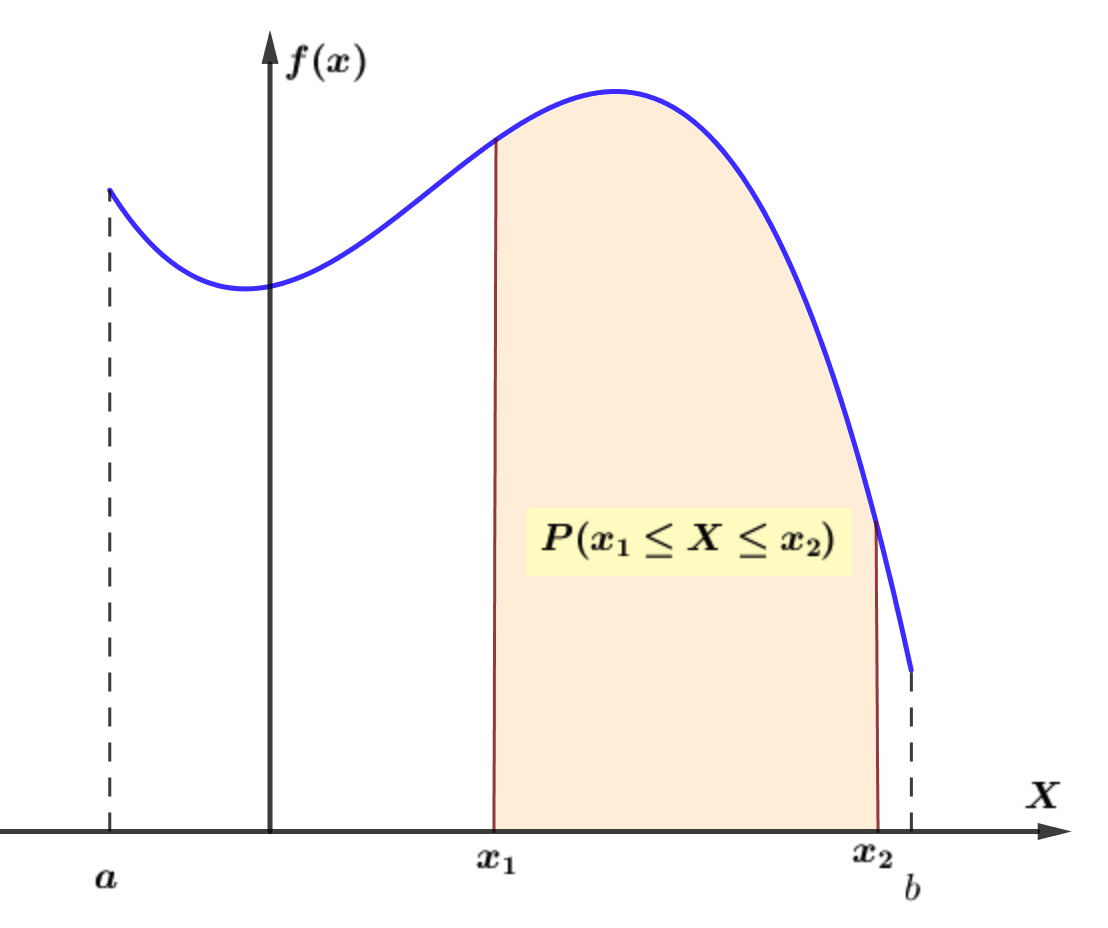
\includegraphics[width=.5\textwidth]{imagenes/imagenes04/T04IM10.png}
	\caption*{\small{$\displaystyle F(B)=P(X\le b)=P(a\le X \le b)=\int_a^b f(x)\ \dd x=1 $}}
	\end{figure}
	
\begin{theorem}
.	$$ \boldsymbol{ \displaystyle \int_{-\infty}^{+\infty} \ f(x) \ \dd x \ = \ 1 } $$	
\end{theorem}


\begin{multicols}{2}

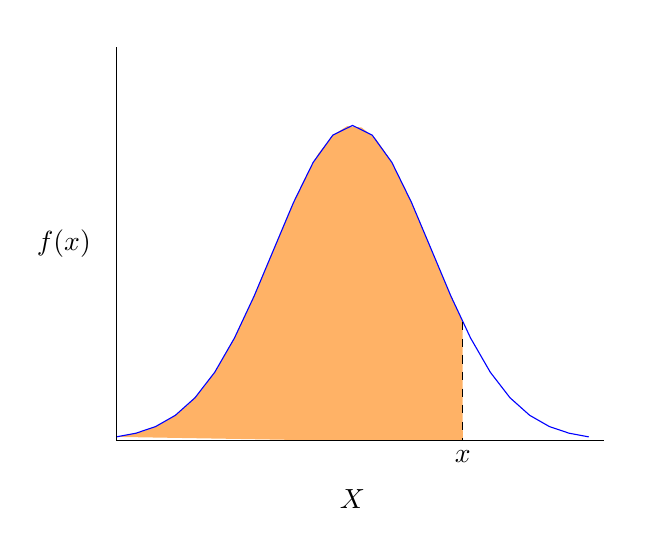
\begin{tikzpicture}
% define normal distribution function 'normaltwo'
\def\normaltwo{\x,{4*1/exp(((\x-3)^2)/2)}}

% input y parameter
\def\y{4.4}

% this line calculates f(y)
\def\fy{4*1/exp(((\y-3)^2)/2)}

% Shade orange area underneath curve.
\fill [fill=orange!60] (2.6,0) -- plot[domain=0:4.4] (\normaltwo) -- ({\y},0) -- cycle;

% Draw and label normal distribution function
\draw[color=blue,domain=0:6] plot (\normaltwo) node[right] {};

% Add dashed line dropping down from normal.
\draw[dashed] ({\y},{\fy}) -- ({\y},0) node[below] {$x$};

% Optional: Add axis labels
\draw (-.2,2.5) node[left] {$f(x)$};
\draw (3,-.5) node[below] {$X$};

% Optional: Add axes
\draw[] (0,0) -- (6.2,0) node[right] {};
\draw[] (0,0) -- (0,5) node[above] {};

\end{tikzpicture}

$\quad$

$\quad$

$$ F(X)=P(X\le x)=\displaystyle \int_a^x f(x) \ \dd x$$

$\quad$
\end{multicols}



\subsection{Esperanza matemática y desviación típica de una v.a. continua}


\begin{definition}
.	Par X v.a. continua, se definen	

\vspace{2mm} \hspace{1cm} \textbf{Esperanza matemática} $\ \mu=E(X)=\displaystyle \int_{-\infty}^{+\infty}\ x\cdot f(x)\ \dd x$

\vspace{2mm} \hspace{1cm} \textbf{Varianza} $\ \sigma^2=\displaystyle \int_{-\infty}^{+\infty}\ (x -\mu)^2\cdot f(x)\ \dd x$
$\quad$ \textbf{Desviación típica} $\ \sigma \ =\  \sqrt{\sigma^2}$

\vspace{2mm} Si X toma valores en [a,b], los límites de integración son `a'. y `b'. 
\end{definition}

En las distribuciones más usuales, los valores de estas integrales suelen venir tabulados (en forma de tablas).


\section{Distribución Normal}

Existen multitud de distribuciones de variable aleatoria continua, la más importante es la distribución Normal. Veremos antes algunas más sencillas.


\textbf{\large{Distribución uniforme}} \normalsize{(continua)}.

Esta distribución es la más sencilla de las distribuciones continuas, surge al considerar una variable aleatoria que toma valores \emph{equiprobables} en un intervalo finito y su nombre se debe al hecho de que la densidad de probabilidad de esta variable aleatoria es uniforme (constante) sobre todo el intervalo de definición.

\vspace{4mm}
\begin{definition}
.	Se dice que una v.a. X se distribuye según una \textbf{distribución uniforme} en el intervalo [a,b], $\boldsymbol{X \leadsto U[a,b]}$, si la probabilidad de que tome cualquier subintervalo de valores es proporcional a la longitud de dicho subintervalo.

\vspace{2mm} \textbf{Función densidad:} $\quad f(x)=\dfrac 1 {b-a}; \ \ \  a<x<b; \quad 0$ en cualquier otro caso.

\vspace{2mm} \textbf{Función de distribución:} $\quad F(X)=\begin{cases}
\ 0& x<a \\ \ \dfrac{x-a}{b-a} & a < x < b \\ \ 1 & x>b	
\end{cases}$

\vspace{2mm} \textbf{Esperanza matemática:} $\quad E(X)=\dfrac{a+b}2$

\vspace{2mm} \textbf{Desviación típica:} $\quad \sigma= \sqrt{\dfrac{(b-a)^2}{12}}$

	\begin{figure}[H]
	\centering
	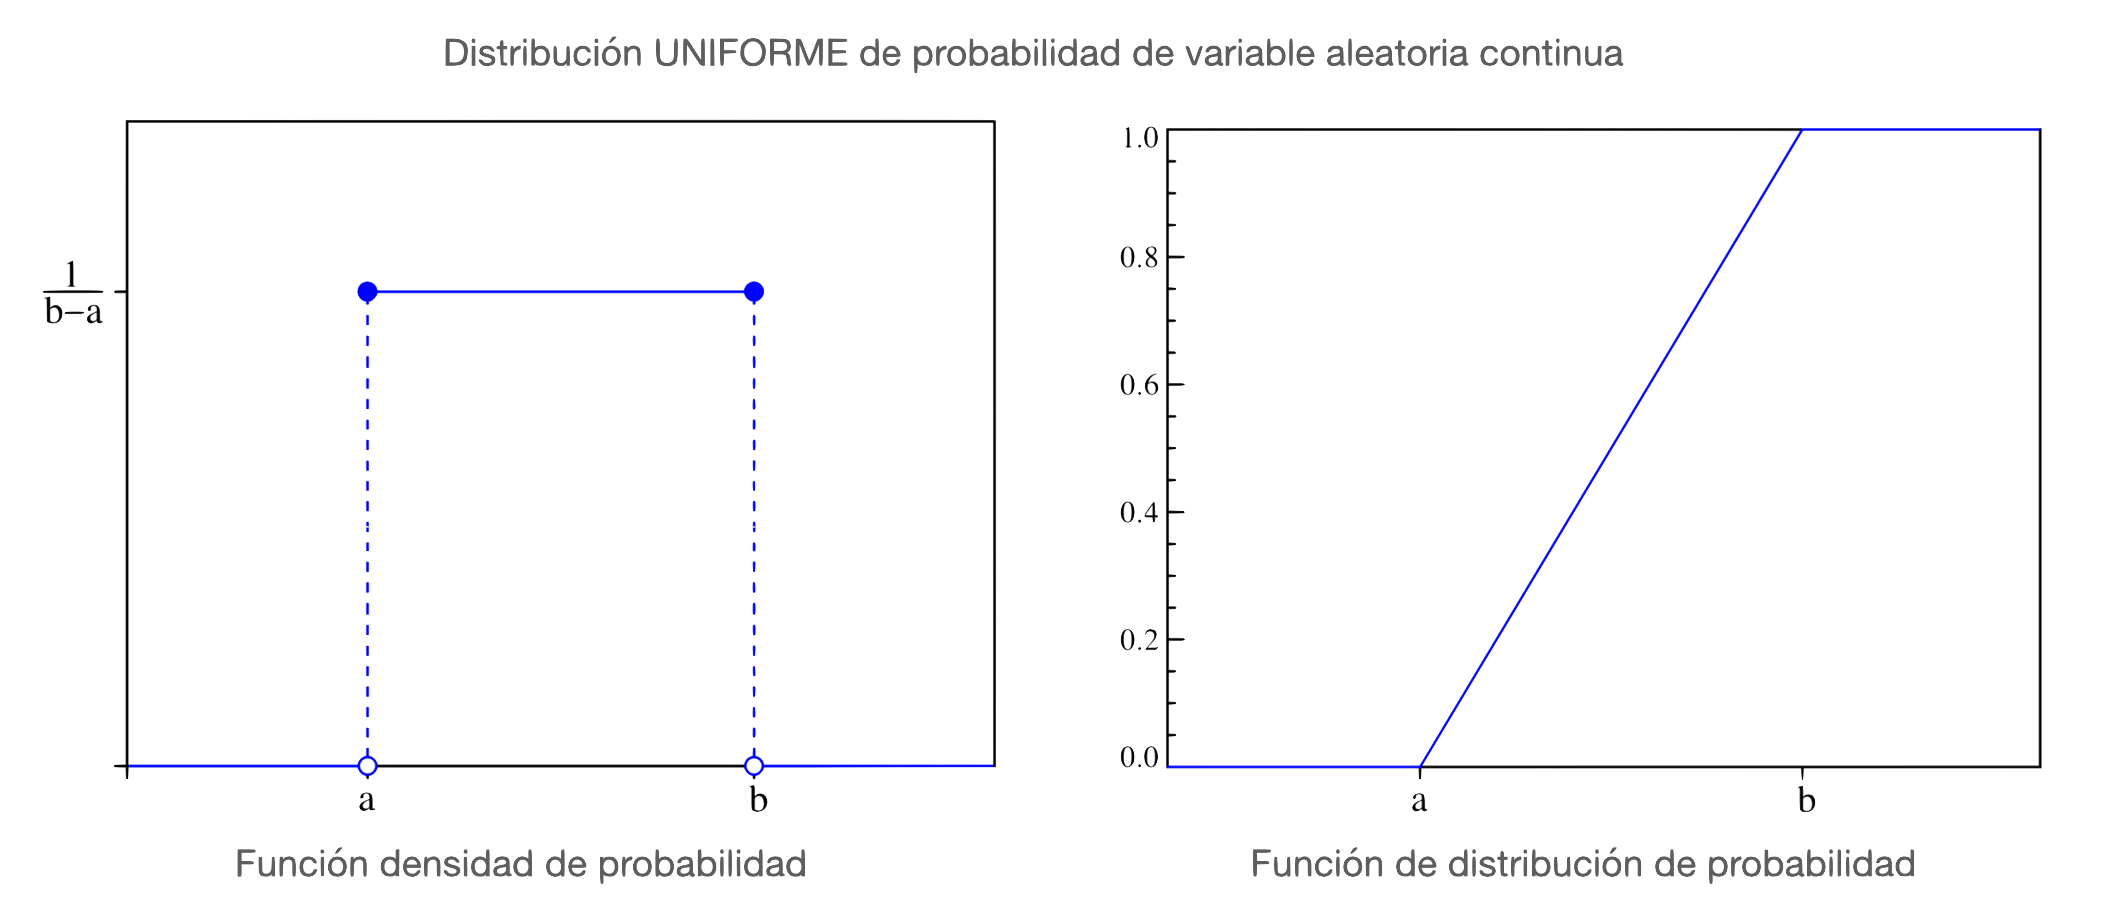
\includegraphics[width=.9\textwidth]{imagenes/imagenes04/T04IM42.png}
	\end{figure}
\end{definition}

Como en todas la v.a. continuas, el intervalo de definición de la distribución uniforme puede ser abierto, semiabierto o cerrado.

\vspace{4mm}
\begin{example}
. 	Elegimos un número real al azar entre $[2,6]$ y sea $X=$ ``número seleccionado''. Calcula la probabilidad de que el número elegido sea menor que 5 y calcula la esperanza matemática (el número esperado).

\vspace{2mm} 
\begin{small}
$X\leadsto U([2,6]) \ \to \ P(X\le 5)=\displaystyle \int_2^5 f(x)\ \dd x= \int_2^5 \dfrac 1{6-2}\ \dd x=\int_2^5 \dfrac 1 4 \ \dd x=\dfrac 1 4 \left[ \eval{ x}_2^5 \right.=\dfrac 3 4 = 75\%$

$E(X)= \dfrac{2+6}{2}=\dfrac 8 2 = 4$
\end{small}
\end{example}


\vspace{5mm} \textbf{\large{Distribución exponencial}} \normalsize{.}


Esta distribución suele ser modelo de aquellos fenómenos aleatorios que miden el tiempo que transcurre entre dos sucesos. Por ejemplo, entre la puesta en marcha de un cierto componente y su fallo o el tiempo que transcurre entre dos llegadas consecutivas a un cajero automático.

\vspace{4mm}
\begin{definition}
.	Sea X una v.a. continua que puede tomar valores $x \ge 0$, decimos que X sigue una \textbf{distribución exponencial} de {parámetro $\lambda$} (y se nota $\boldsymbol{X \leadsto e^{\lambda}}$) si su \textbf{función de densidad} está dada por:

\vspace{2mm} \textbf{función densidad:} $\quad f(x)=\lambda \ e^{-\lambda \ x};\ \ x\ge 0; \quad 0$ en cualquier otro caso.

\vspace{2mm} \textbf{función de distribución:} $\quad F(x)=\begin{cases}
\ 1-e^{-\lambda \ x} & x\ge 0 \\ 0 & \text{en otro caso}	
\end{cases}$

\vspace{2mm} \textbf{Esperanza matemática:} $\quad E(X)=\dfrac 1 \lambda$
$\qquad$ \textbf{Desviación típica:} $\quad \sigma= \dfrac 1 \lambda$

\end{definition}

\begin{figure}[H]
	\centering
	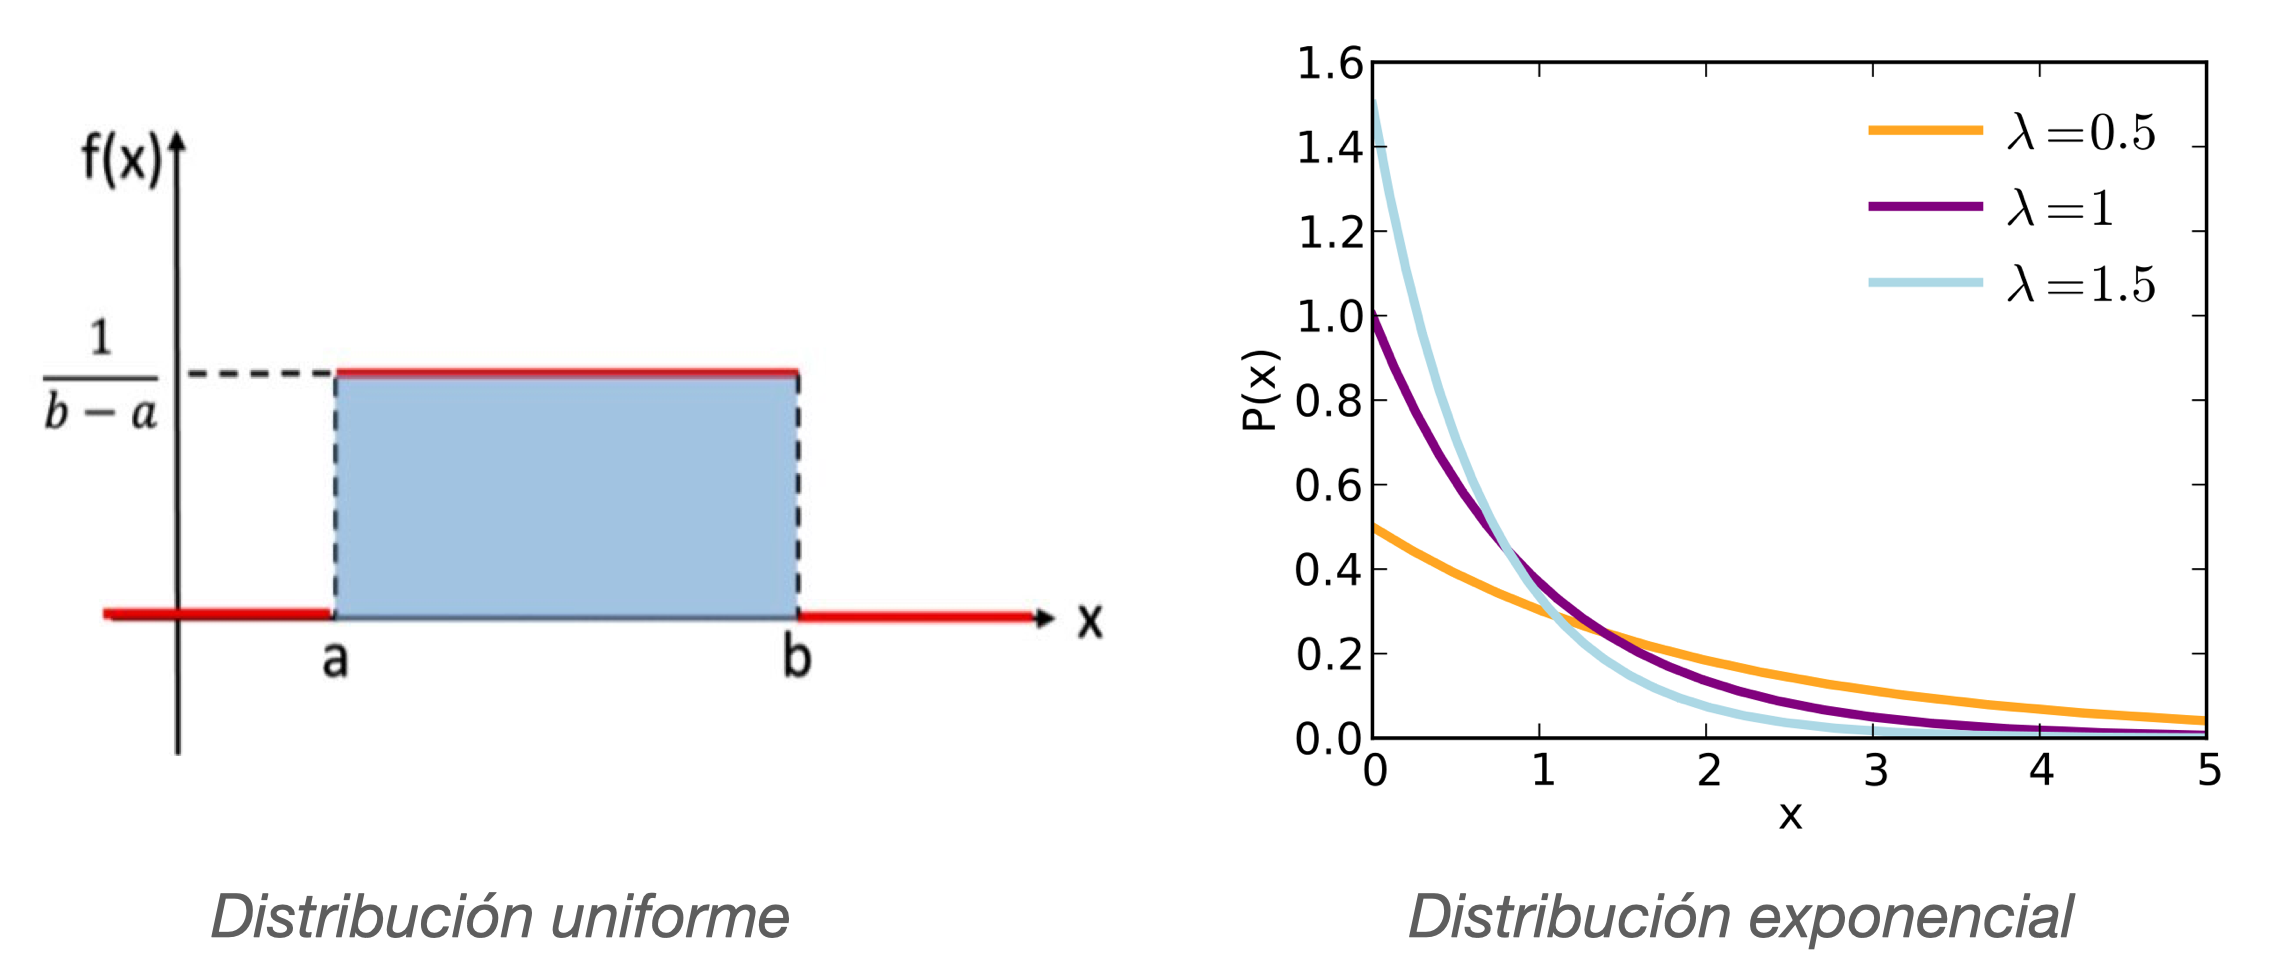
\includegraphics[width=1\textwidth]{imagenes/imagenes04/T04IM11.png}
	\end{figure}
	
\begin{example}
.	El tiempo de vida media de una determinada bombilla sigue una distribución exponencial con media de 100 horas.

?`Cual es la probabilidad de que una bombilla dure más de 30 horas? ?`Y más de 150?

Si cogemos 50 lámparas, ?`Cuántas se espera que duren por lo menos 30 horas?	

\vspace{2mm} Como $E(X)=100=\dfrac 1 \lambda \ \to \ \lambda = \dfrac 1 {100} \ \Rightarrow \ X\leadsto exp(1/100)$


$P(X>30)=1-P(x\le 30)=1-F(30)=1-(1-e^{-30/100})=e^{-30/100}=0.7408\approx 74\%$

$P(X>150)=\cdots=e^{-150/100}=0.2231\approx 22\%$

\vspace{2mm} n=50 bombillas, cada una de ellas con la probabilidad de durar más de 30 horas (exito) igual a p=0.7408 forman una distribución binomial $B(50,0.7408)$, así, el número esperado de éxito de esas bombillas será de $E(X)=n\ p=50\ 0.7408 \approx 37$ bombillas.

\vspace{2mm} \textcolor{gris}{También podríamos haber razonado así: como la duración de las bombillas es independiente de la bombilla elegida, si el que una dure más de 30 horas tiene una probabilidad del 74\% (aprox.), de 50 bombillas durarán más de 30 horas $\to 50 \cdot 74\% \approx 37$ bombillas.}
\end{example}
	
	

\vspace{5mm}\textbf{\Large{\subrayado{\text{Distribución Normal}}}}\large{ \textbf{o de Laplace-Gauss}} \normalsize{.}

En estadística y probabilidad se llama distribución normal, de Gauus o de  Laplace-Gauss a la  distribución de probabilidad de variable aleatoria continua que con más frecuencia aparece en estadística.

La gráfica de su función densidad tiene forma acampanada y es simétrica respecto de la media. Esta curva se conoce con el nombre de \emph{``campana de Gauss} y a su gráfica se le llama `gaussiana'.

La importancia de esta distribución radica en que permite calcular numerosos fenómenos naturales, sociales y psicológicos. Algunos ejemplos asociados a fenómenos que siguen una distribución normal son:


\vspace{-3mm} \begin{itemize}
\vspace{-3mm} \item caracteres morfológicos de individuos como la estatura, peso, etc,
\vspace{-3mm} \item caracteres fisiológicos como el efecto de determinado fármaco,
\vspace{-3mm} \item caracteres sociológicos como el consumo de cierto producto por un grupo de individuos, 
\vspace{-3mm} \item  caracteres psicológicos como el cociente intelectual, 
\vspace{-3mm} \item  nivel de ruido en telecomunicaciones,
\vspace{-3mm} \item errores cometidos al medir determinadas magnitudes,
\vspace{-3mm} \item etc.
\vspace{-3mm} \end{itemize}

La distribución normal es la más extendida en estadística y muchos test estadísticos están basados en ella. 

\vspace{0.4mm}%**************************
\begin{small}
\textcolor{gris}{La distribución normal fue presentada por primera vez por Abraham de Moivre en un artículo del año 1733 en el contexto de cierta aproximación de la distribución binomial para grandes valores de n. Su resultado fue ampliado por Laplace en su libro `Teoría analítica de las probabilidades' (1812) y, en la actualidad, se llama teorema de De Moivre-Laplace}

\textcolor{gris}{El nombre de Gauss se ha asociado a esta distribución porque la usó con profusión cuando analizaba datos astronómicos y algunos autores le atribuyen su descubrimiento.}

\textcolor{gris}{ El nombre de ``campana'' viene de Esprit Jouffret que usó el término `bell surface' por primera vez para referirse a esta curva. El nombre \emph{distribución normal} fue otorgado, independientemente, por Charles S. Peirce, Francis Galton y Wilhelm Lexis por 1875.}
\end{small}


	\begin{figure}[H]
	\centering
	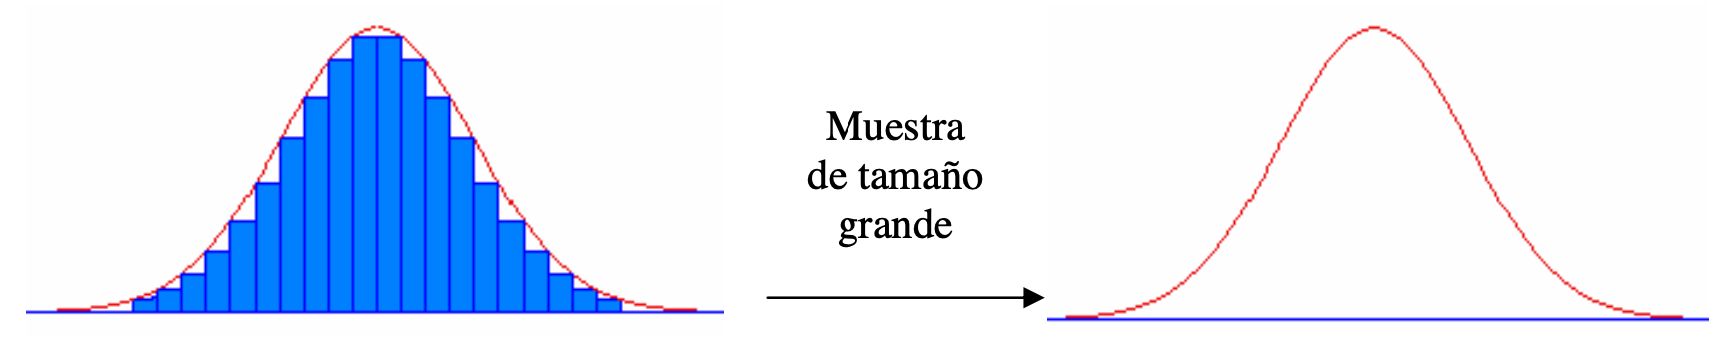
\includegraphics[width=1\textwidth]{imagenes/imagenes04/T04IM12.png}
	\caption*{Muchas distribuciones estadísticas pueden aproximarse a una distribución normal.}
	\end{figure}

\vspace{0.4mm} %*************************************************	
\begin{destacado}
	\emph{En muchas ocasiones encontraremos que un conjunto de valores se corresponde con una distribución normal o muy aproximada a la normal. Además, veremos \emph{(próximo tema)} que, en determinadas circunstancias, el proceso de `muestreo' garantiza la normalidad aunque la población de la que se extrae la muestra no sea normal. Esto aumenta más aún la importancia del papel de la normal.}
\end{destacado}

\vspace{0.4mm} %*************************************************
\begin{definition}
.	Una v.a. continua $\boldsymbol{X}$ se distribuye según una 	\textbf{Normal} de media $\mu$ y desviación típica $\sigma$, que denotamos por $\subrayado{ \ \boldsymbol{X \leadsto N(\mu , \sigma)}\, }$ si su función de densidad de probabilidad es:

$$\subrayado{ \  \boxed{ \   \boldsymbol{ f(x)\ = \ \dfrac{1}{\sqrt{2 \pi}\ \sigma} \ e^{-\dfrac{(x-\mu)^2}{2 \sigma^2}} }  \ } \ } \qquad \ \ x\in \mathbb R;\ \quad  \mu \in \mathbb R;\ \ \sigma > 0$$
\end{definition} 

\vspace{10mm} %*************************************************
	\begin{figure}[H]
	\centering
	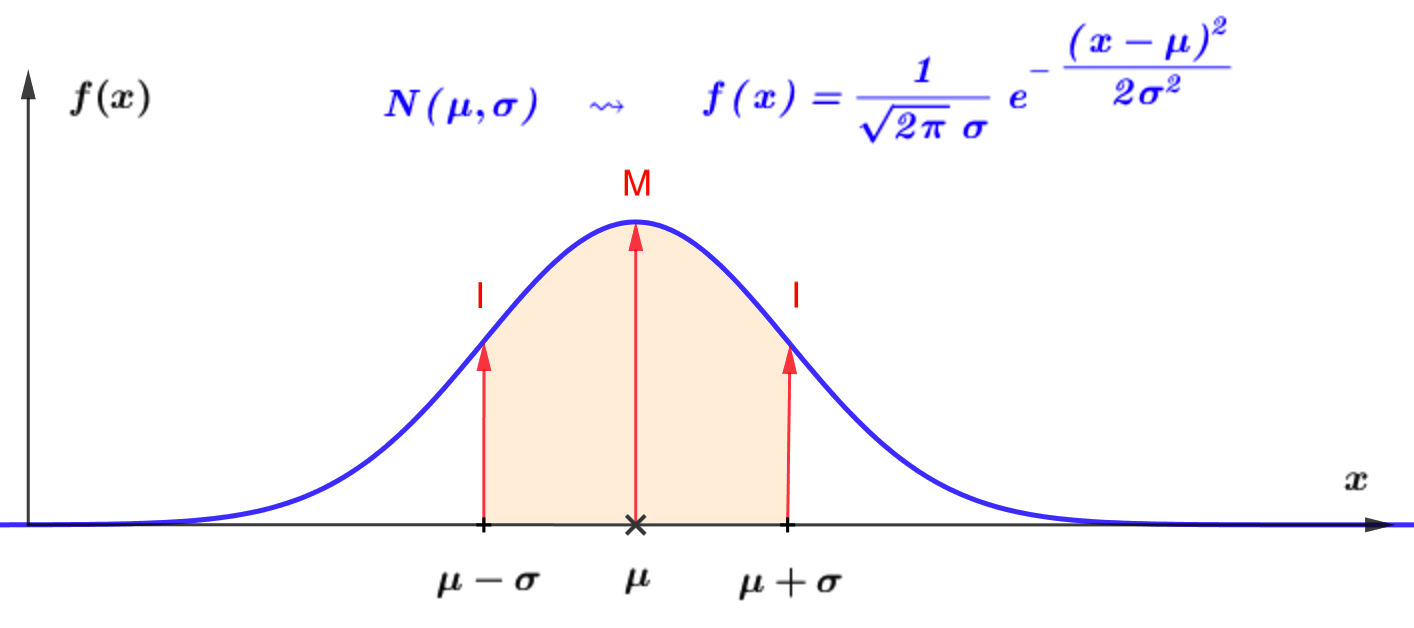
\includegraphics[width=.9\textwidth]{imagenes/imagenes04/T04IM13.png}
	\caption*{Curva normal, \emph{`campana de Gauss'}.}
	\end{figure}
	
\begin{theorem}
.	\textbf{Propiedades de la `campana de Gauss'} (de la Normal).

\begin{enumerate}
\item El eje OX (y=0) es Asíntota Horizontal de la curva normal.
\item Presenta un \textbf{máximo} en $x=\mu$ \textcolor{gris}{$\quad M_{ax} \left( \mu, \dfrac {1}{\sqrt{2\pi}\sigma} \right) $}
\item Hay dos puntos de \textbf{inflexión} en $x=\mu \pm \sigma$
\item La curva normal es \textbf{simétrica} respecto de la recta $x=\mu$: $\quad f(x-\mu)=f(x+\mu)$
\item En la curva normal \textbf{coinciden media, mediana y moda}.
\item El área total bajo la curva es uno: $\ \displaystyle \int_{-\infty}^{+\infty} f(x)\ \dd x=1$
\item \textcolor{gris}{ Si $Y=aX+B$ y $X\leadsto N(\mu,\sigma) \ \Rightarrow \ Y\leadsto N(a\mu +b, a\sigma)$ }
\item \textcolor{gris}{ Si $X_1\leadsto N(\mu_1,\sigma_1)$ y $X_2\leadsto N(\mu_2,\sigma_2) \ \Rightarrow \ Y=X_1+X_2\leadsto N(\mu_1+\mu_2, \sqrt{\sigma_1^2+\sigma_2^2})$ }
\item \textcolor{gris}{ \textbf{Teorema central del límite} (próximo tema):  }

\textcolor{gris}{Si $X_1,X_2,\cdots ,X_n $ son $n$ v.a. independientes con media $\mu$ y desviación típica $\sigma$, entonces:}

\textcolor{gris}{
$$\displaystyle \sum_{i=1}^n X_i \leadsto N(n\mu, \sigma \sqrt
n);\qquad \qquad  \dfrac{\sum_{i=1}^n X_i}{n} \leadsto N \left( \mu, \dfrac{\sigma}{\sqrt{n}} \right)  $$
}
\end{enumerate}	
\end{theorem}
	
\vspace{10mm}
%*********GAUSSIANA. 1,2,3 sigmas **************************
\begin{center}
\pgfmathdeclarefunction{gauss}{2}{\pgfmathparse{1/(#2*sqrt(2*pi))*exp(-((x-#1)^2)/(2*#2^2))}%
}
\begin{tikzpicture}
\begin{axis}[no markers, domain=0:10, samples=100,
axis lines*=left, xlabel=Standard deviations, ylabel=Frequency,,
height=6cm, width=10cm,
xtick={-3, -2, -1, 0, 1, 2, 3}, ytick=\empty,
enlargelimits=false, clip=false, axis on top,
grid = major]
\addplot [fill=cyan!20, draw=none, domain=-3:3] {gauss(0,1)} \closedcycle;
\addplot [fill=orange!20, draw=none, domain=-3:-2] {gauss(0,1)} \closedcycle;
\addplot [fill=orange!20, draw=none, domain=2:3] {gauss(0,1)} \closedcycle;
\addplot [fill=blue!20, draw=none, domain=-2:-1] {gauss(0,1)} \closedcycle;
\addplot [fill=blue!20, draw=none, domain=1:2] {gauss(0,1)} \closedcycle;
\addplot[] coordinates {(-1,0.4) (1,0.4)};
\addplot[] coordinates {(-2,0.3) (2,0.3)};
\addplot[] coordinates {(-3,0.2) (3,0.2)};
\node[coordinate, pin={68.2\%}] at (axis cs: 0, 0.4){};
\node[coordinate, pin={95\%}] at (axis cs: 0, 0.3){};
\node[coordinate, pin={99.7\%}] at (axis cs: 0, 0.2){};
\node[coordinate, pin={34.1\%}] at (axis cs: -0.5, 0){};
\node[coordinate, pin={34.1\%}] at (axis cs: 0.5, 0){};
\node[coordinate, pin={13.6\%}] at (axis cs: 1.5, 0){};
\node[coordinate, pin={13.6\%}] at (axis cs: -1.5, 0){};
\node[coordinate, pin={2.1\%}] at (axis cs: 2.5, 0){};
\node[coordinate, pin={2.1\%}] at (axis cs: -2.5, 0){};
\end{axis}
\end{tikzpicture}
\end{center}

%***************FIN GAUSSIANAS 1,2,3, sigmas ***************


En una distribución normal, la probabilidad de que la variable se aleje menos de una desviación típica de la media es del 68.2\%. 

\begin{destacado}
\begin{adjustwidth}{10pt}{10pt}
	En estadística descriptiva decíamos, en la sección \emph{\ref{mediaydesviacion} interpretación conjunta de media y desviación típica}, que los individuos de la distribución que se alejan menos de una desviación típica de la media eran alrededor de los 2/3 de la población, es decir, del 67\% de la población. Ello es debido a que muchas distribuciones estadísticas se aproximan a una distribución teórica Normal.
\end{adjustwidth}
\end{destacado}



Alejarse menos de dos desviaciones típicas tiene una probabilidad del 95\% y tres desviaciones típicas del 99.7\%. 

\begin{small}$$P(\mu-\sigma\le x \le \mu+\sigma)=68.2\%); \quad P(\mu-2\sigma\le x \le \mu+2\sigma)=95\%); \quad P(\mu-3\sigma\le x \le \mu+3\sigma)=99.7\%$$\end{small}


\begin{destacado}
\begin{adjustwidth}{10pt}{10pt}
A mayor desviación típica, los datos son más dispersos respecto de la media. Por ello, las curvas normales son más achatadas a mediada que aumenta la desviación típica indicando la mayor dispersión de los datos.  Los distintos valores de la media hacen que las curvas normales estén centradas en distintos puntos.
\end{adjustwidth}
\end{destacado}



% diferentes gaussianas *************************
\begin{multicols}{2}
\pgfmathdeclarefunction{gauss}{2}{\pgfmathparse{1/(#2*sqrt(2*pi))*exp(-((x-#1)^2)/(2*#2^2))}%
}
\begin{tikzpicture}
\begin{axis}[every axis plot post/.append style={
  mark=none,domain=-2:4.5,samples=500,smooth}, % All plots: from -2:2, 50 samples, smooth, no marks
  axis x line*=bottom, % no box around the plot, only x and y axis
  axis y line*=left, % the * suppresses the arrow tips
  enlargelimits=upper] % extend the axes a bit to the right and top
  \addplot {gauss(0,0.5)};
  \addplot {gauss(1,0.75)};
  \addplot {gauss(1.5,1.25)};
\end{axis}
\end{tikzpicture}


\textcolor{blue}{$$\boldsymbol{N(0,0.5)}$$}

%$\quad$

\textcolor{red}{$$\boldsymbol{N(1,0.75)}$$}

%$\quad$

\textcolor{brown}{$$\boldsymbol{N(1.5,1.25)}$$}
\end{multicols}
% \fin diferentes gaussianas *******************

\subsection{Normal standard \small{(típica o tipificada)}}\normalsize{\textcolor{white}{.}}

\begin{definition}
.	$$ \text{Si } \mu=0 \text{ y } \sigma=1 \ \to \ N(0,1):\quad f(x)=\dfrac{1}{\sqrt{2\pi}} \ e^{-\dfrac{x^2}{2}}$$

$$\text{Ahora, } \quad F(x)=P(X\le x)=\dfrac{1}{\sqrt{2\pi}} \ \displaystyle \int_{-\infty}^x e^{-x^2/2}\ \dd x \quad \to \quad  \text{TABLAS}$$
\end{definition}

%\vspace{10mm}%****************************************
	\begin{figure}[H]
	\centering
	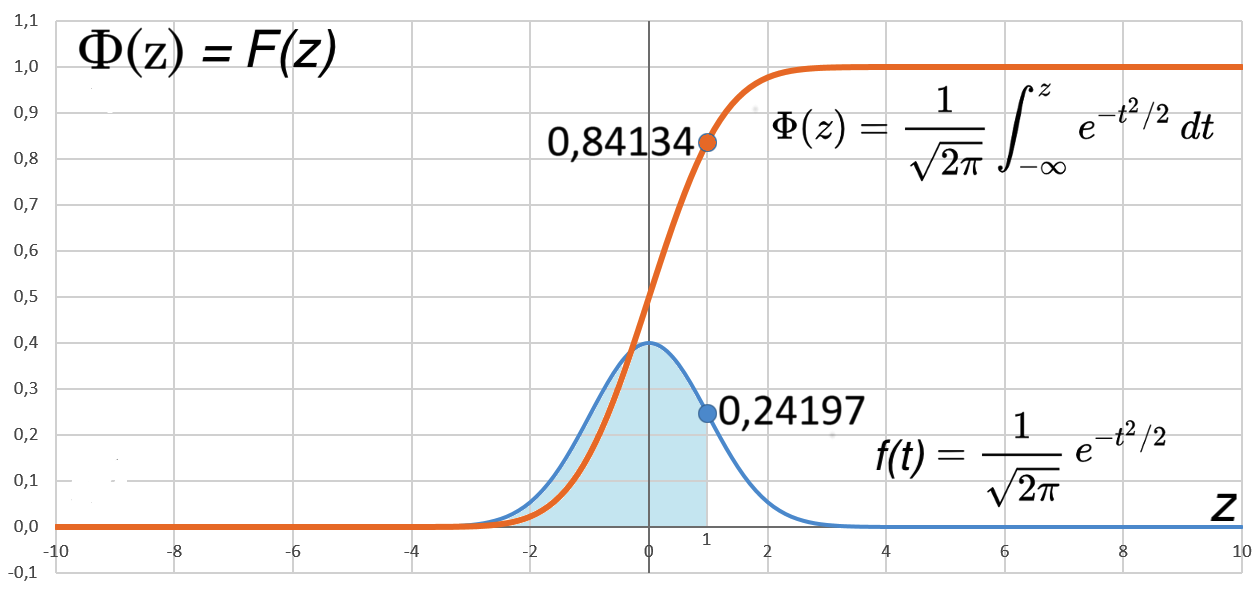
\includegraphics[width=.75\textwidth]{imagenes/imagenes04/T04IM14.png}
	\end{figure}

%\vspace{10mm}%**************************************** 
Sería muy complicado elaborar tablas que proporcionen la probabilidad de cada uno de los casos distintos que se pueden presentar con las distribuciones normales; lo que sí existe es una alternativa sencilla que evita estos problemas cuando tenemos un conjunto de valores que tiende a tomar un comportamiento de tipo normal. Y para ello sólo utilizamos un ``miembro'' de la familia de distribuciones normales: aquella cuya $\mu = 0$  y una $\sigma = 1$. Esta distribución se conoce como \textbf{Distribución Normal Estándar}, para ella si está tabulada la función de distribución. 

%\vspace{4mm} Aprenderemos a manejar estas tablas para calcular probabilidades en la distribución normal típica y veremos como 
todas las distribuciones pueden convertirse a la estándar por medio del proceso que llamaremos \emph{`tipificación de la variable'} y así poder calcular probabilidades en cualquier distribución normal $N(\mu,\sigma)$.




\begin{theorem}
.	\textbf{Propiedades de la N(0,1)}	

\begin{enumerate}
\item Es simétrica respecto de $x=0: \quad f(-x)=f(x)$
\item Tiene un $M_{ax}=(0,0.4)$
\item Tienen inflexiones en $x=\pm 1$
\item $y=0$ es su Asíntota Horizontal
\item !`Importante!: $\quad \bold{F(-x)=1-F(x)}$	
\end{enumerate}

\end{theorem}

	\begin{figure}[H]
	\centering
	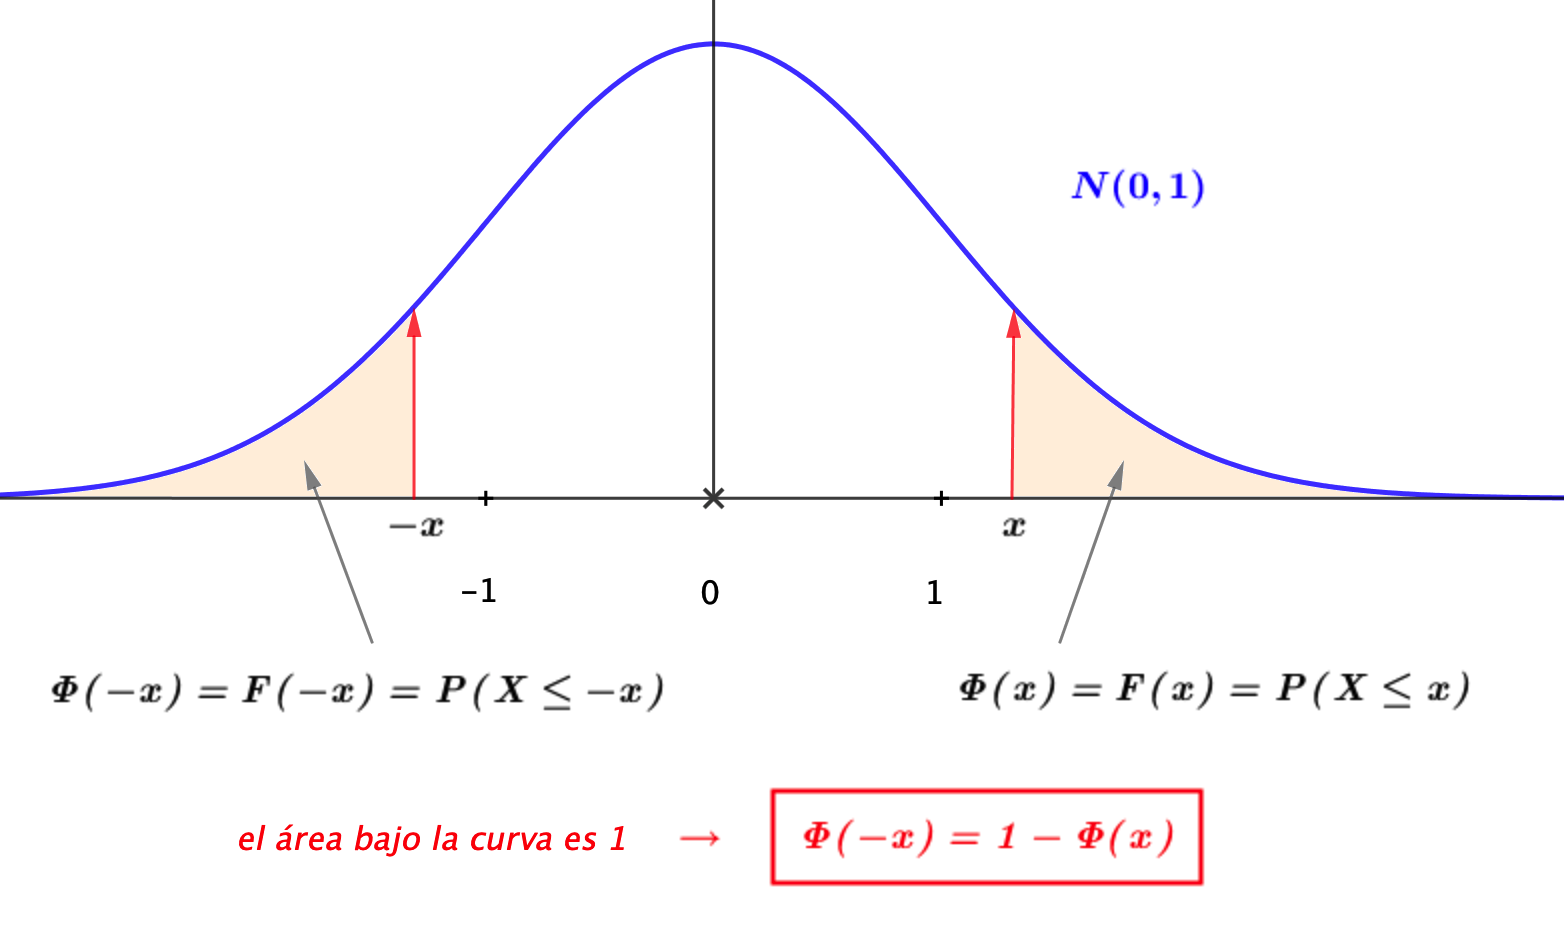
\includegraphics[width=.7\textwidth]{imagenes/imagenes04/T04IM15.png}
	\end{figure}

%\vspace{5mm}%**************************************** 
	\begin{figure}[H]
	\centering
	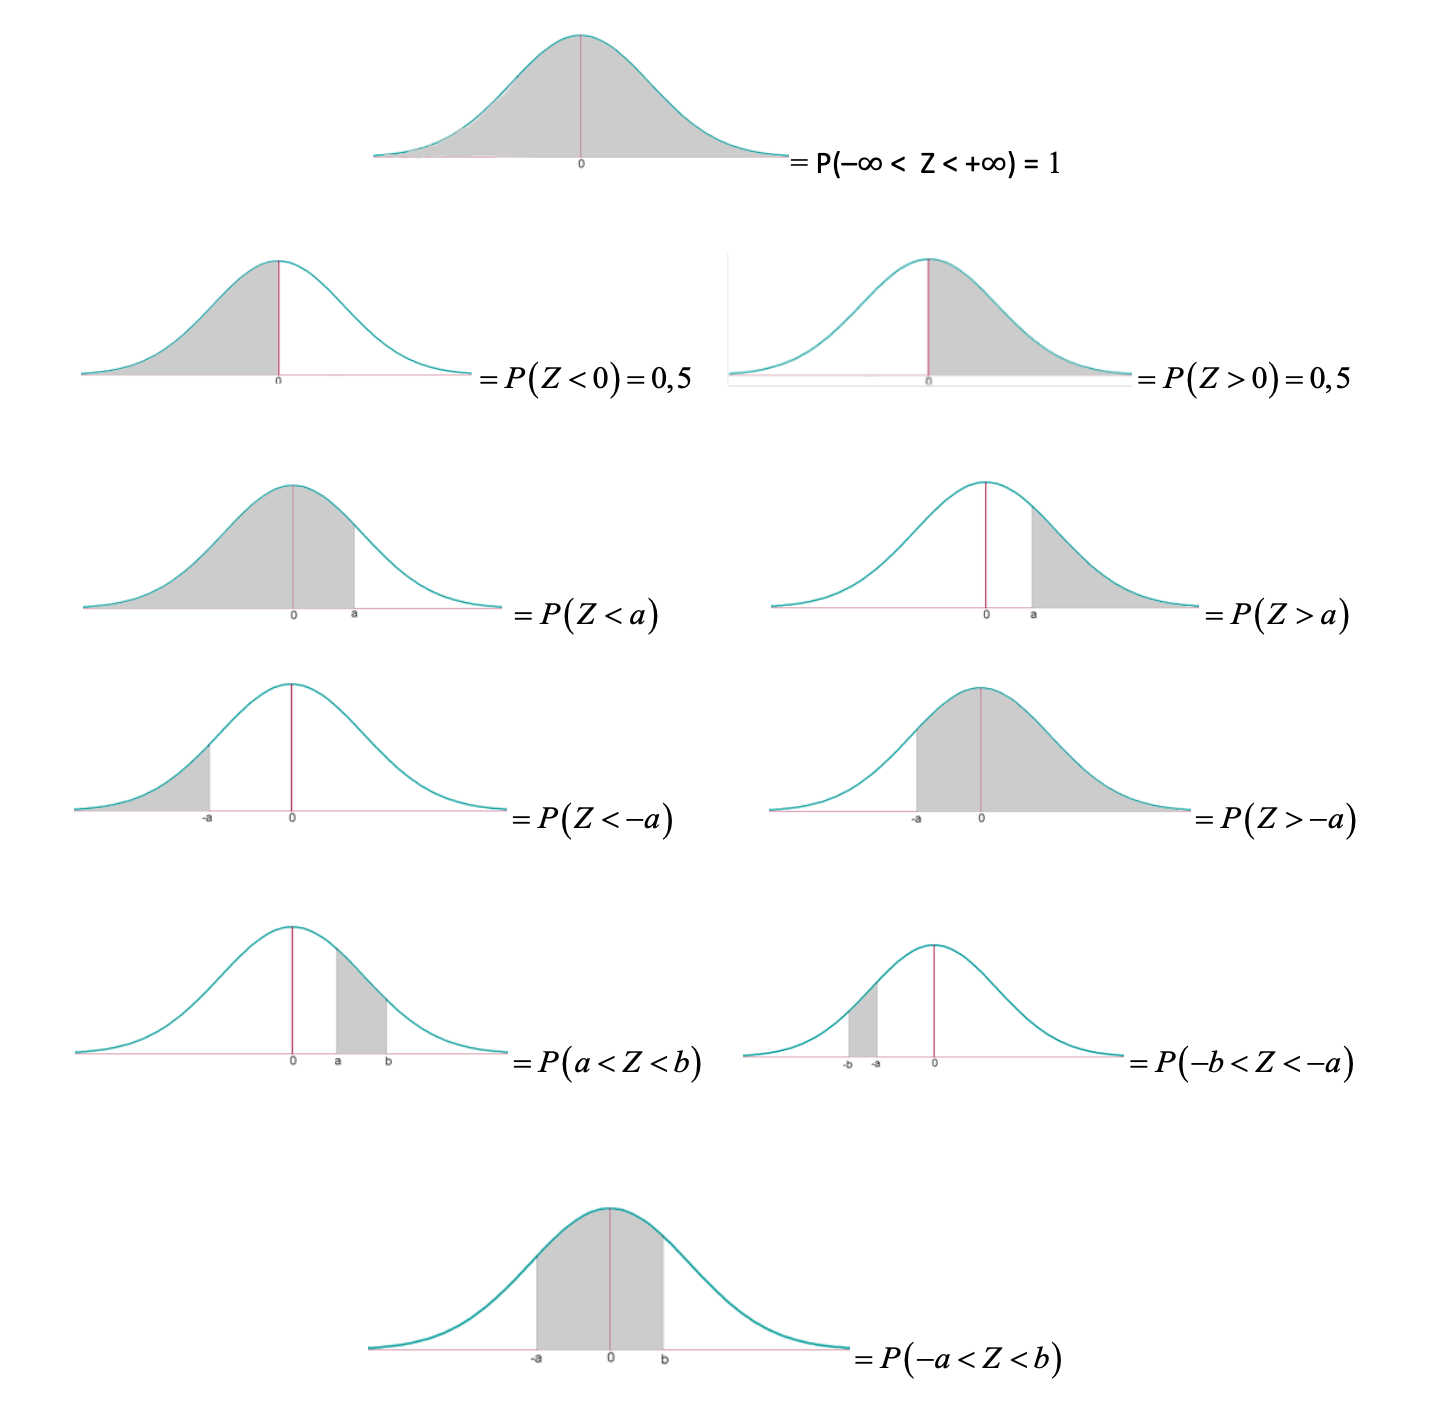
\includegraphics[width=1\textwidth]{imagenes/imagenes04/T04IM16.png}
	\caption*{\small{Simetrías en el cálculo de probabilidades en N(0,1)}}
	\end{figure}

\newpage
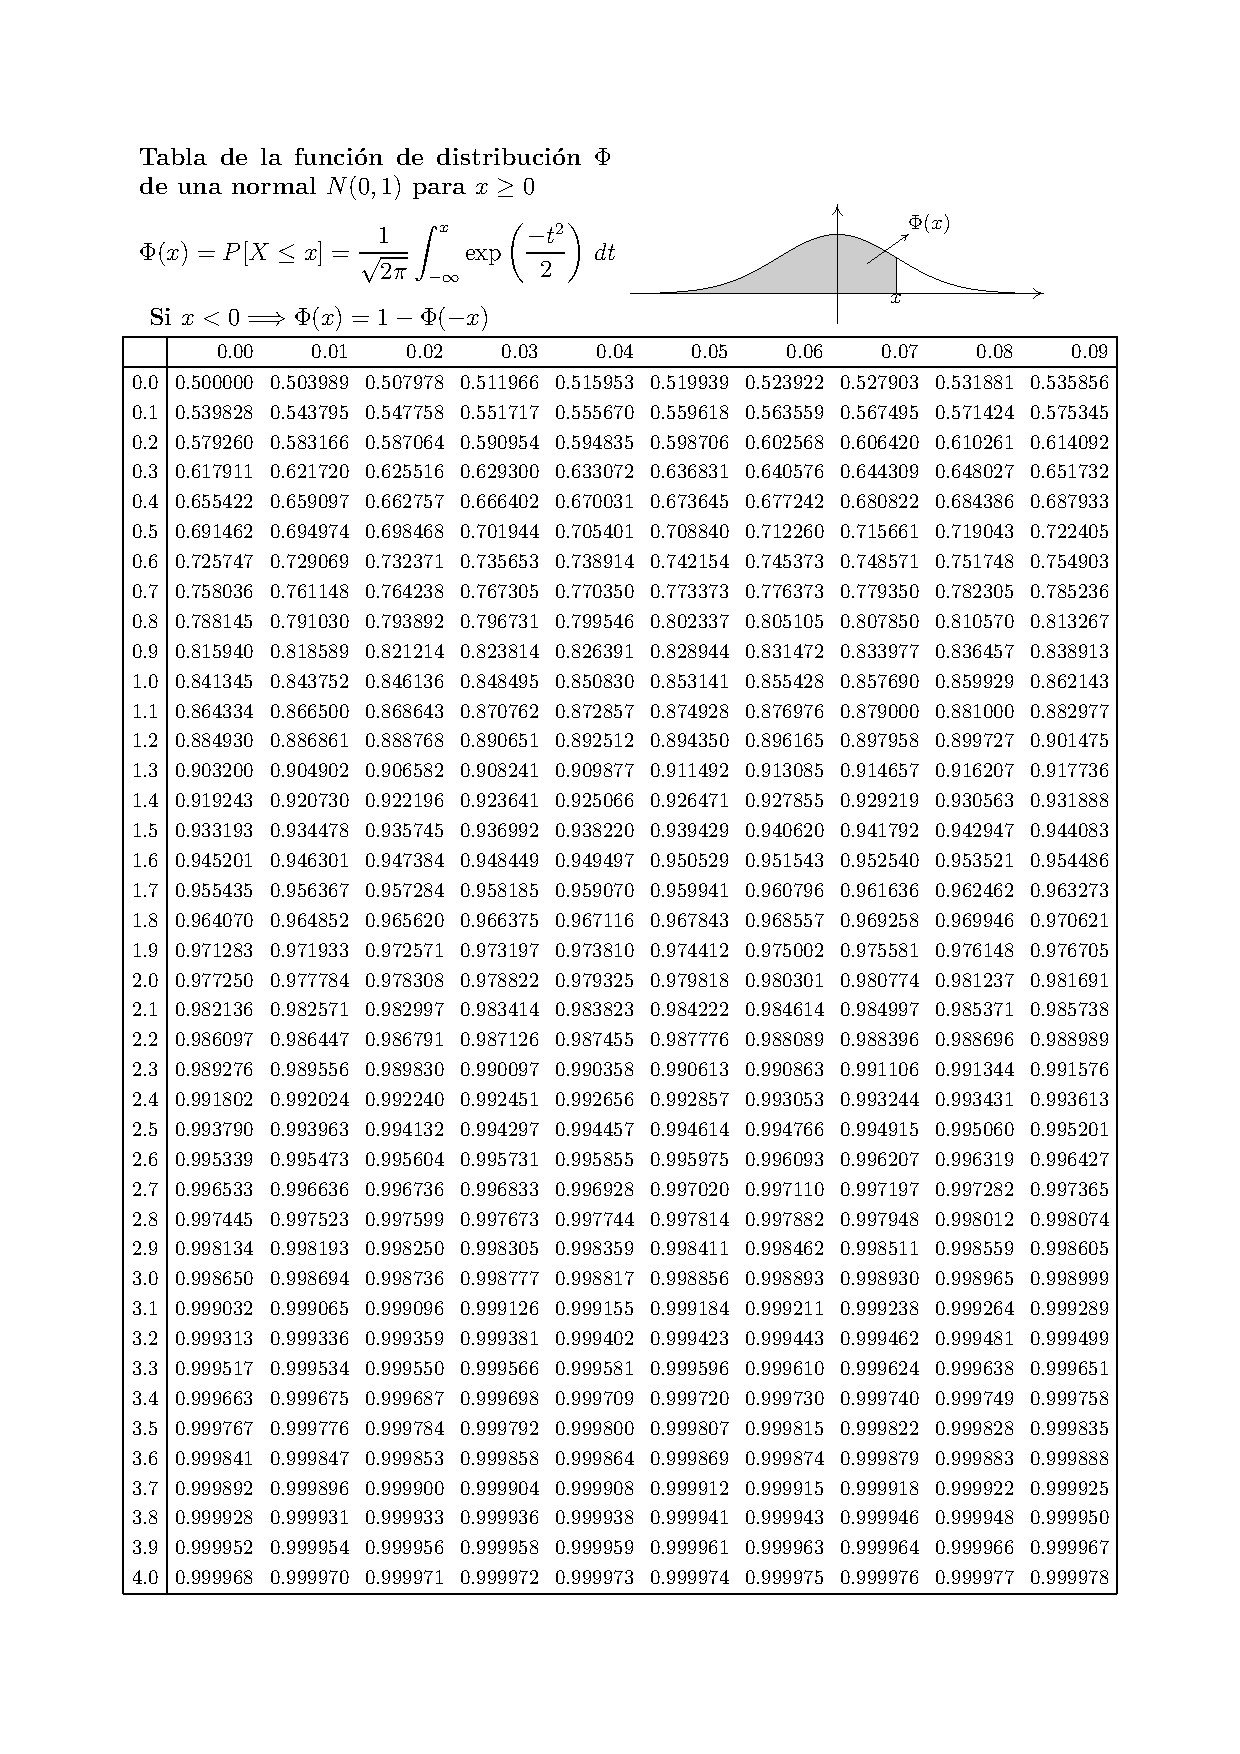
\includepdf[pages=-]{imagenes/imagenes04/normal00.pdf}






\newpage
\begin{large} \textbf{Cálculo de probabilidades en N(0,1)} \end{large}

Como se observa, las probabilidades de que la variable $z$ tome un determinado valor menor (o menor o igual) que $k$ está tabulada en $[0,+\infty[$, en realidad hasta $k=4.09$. Para valores mayores esta probabilidad es prácticamente 1 (con precisión hasta las millonésimas). Para calcular probabilidades para $z<0$ o para $z$ comprendida entre dos valores, $a<z<b$, usaremos las propiedades de simetría de la curva normal.

\begin{example}
.	Directamente e las tablas, \textcolor{red}{$P(z<1,37)=0.914657$}, y a la inversa, \textcolor{blue}{$P(z<k)=0.698468 \to k=0.52$}, como puede observarse en la siguiente figura.

	\begin{figure}[H]
	\centering
	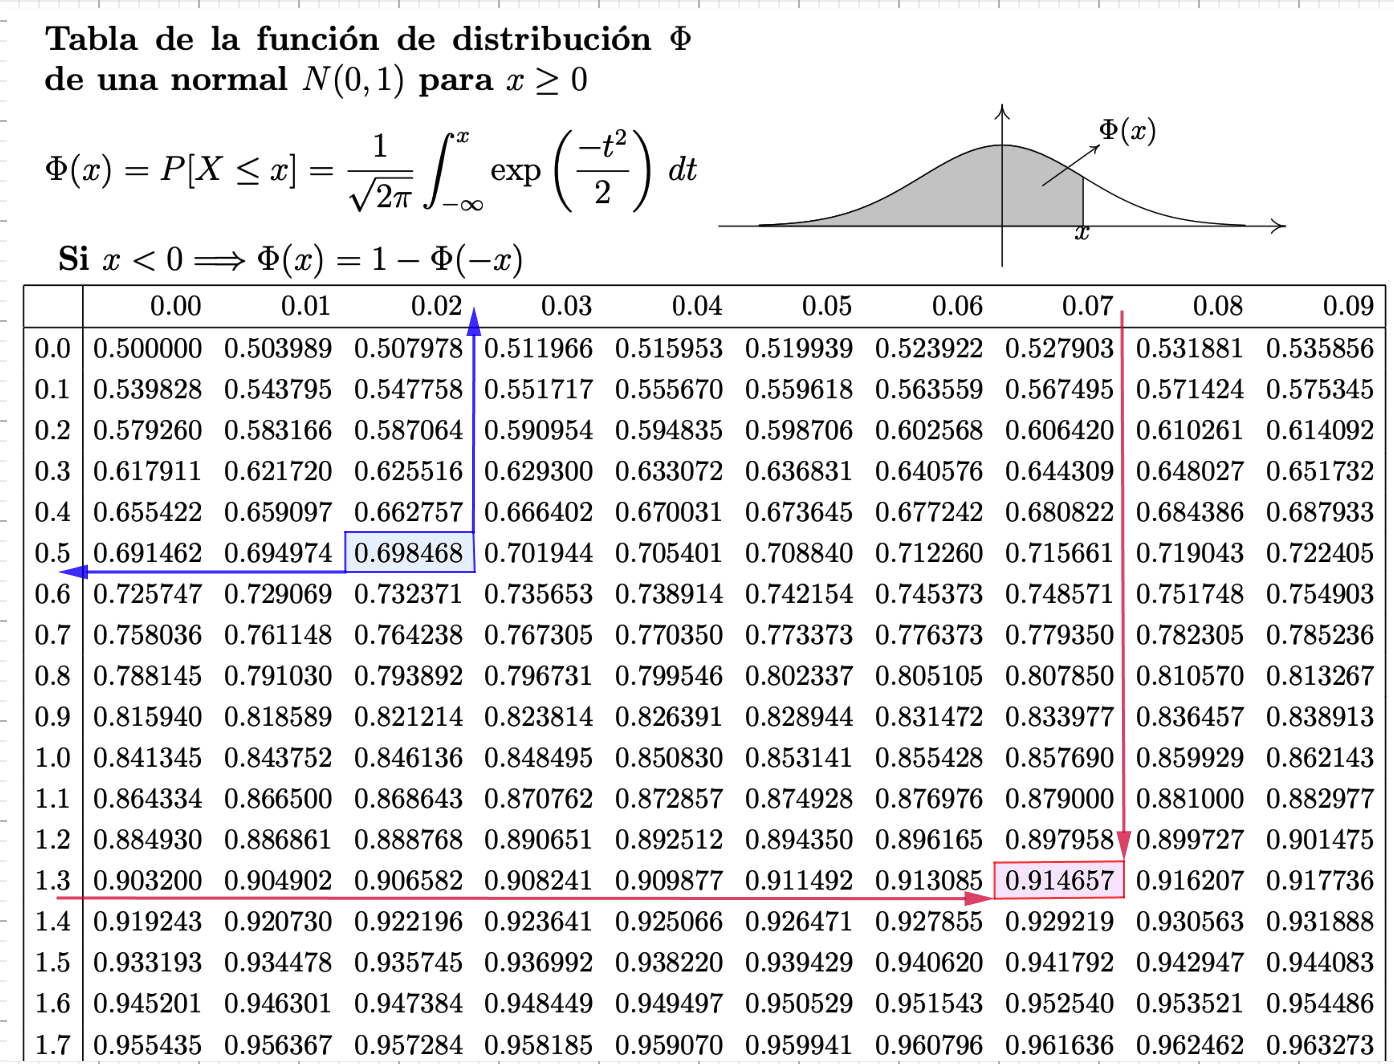
\includegraphics[width=.95\textwidth]{imagenes/imagenes04/T04IM17.png}
	\end{figure}
\end{example}


\begin{ejemplo}


\vspace{4mm} \begin{ejre}
En una N(0,1), calcular las siguientes probabilidades:

$\quad a)\ \ p(z<2.05);\quad b)\ \ p(z\ge 1.27); \quad c)\ \ p(z\le -0.36);\quad d)\ \ p(z> -2.75)$

$\quad e)\ \ p(0.23<z\le 2.17);\qquad f)\ \ p(-1.74<z<-0.92);\qquad g)\ \ p(-1.42<z \le 1)$

\scriptsize{Nótese que en las tablas que estamos usando llaman a la función de distribución $F(z)=\Phi(z)$, usaremos esta notación}\normalsize{.}

\rule{250pt}{0.1pt}

Las desigualdades no im porta que sean o no estrictas ($\ < \text{ ó } \le \ $) ya que en v.a. continua la probabilidad de que la variable tome un valor concreto es cero: 

$$\ p(z\le k)= p(z<k)+\cancelto{0}{p(z=k)};\quad p(z\ge k)=p(z>k); \quad p(a\le z\le b)=p(a<z<b)$$

Acompañaremos cada cálculo con un dibujo y, de este modo, no hará falta memorizar nada. Representaremos por $\Phi$ el valor de la función de distribución, como en las tablas ($\Phi(z)=F(z)$).

Recordar: la curva (campana de Gauss) es simétrica y el área total que encierra es 1. Con la tabla, el cálculo de probabilidades se reduce al cálculo de áreas.
 
 \begin{multicols}{2}
 $a)\ \ p(z<2.05)=$
 
 $\quad =\Phi(2.05)=$
 
 $\quad =0.979818$
 
 \begin{figure}[H]
	\centering
	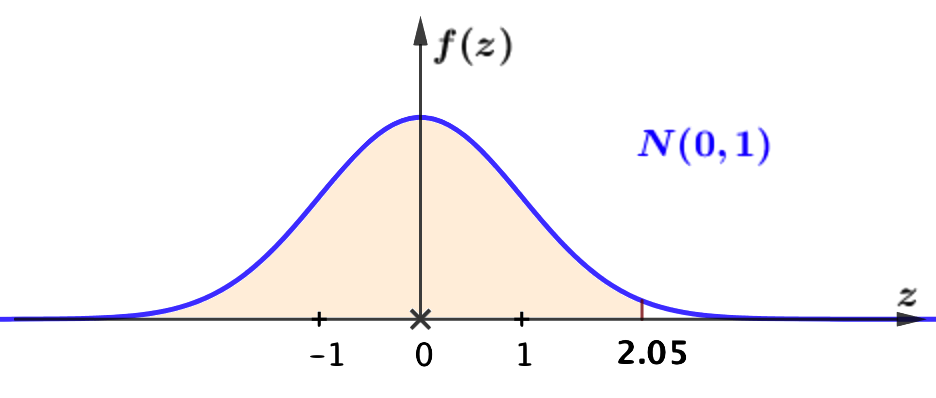
\includegraphics[width=.5\textwidth]{imagenes/imagenes04/T04IM18.png}
	\end{figure}
 	
 \end{multicols}
 
 \begin{multicols}{2}
 $b)\ \ p(z\ge 1.27)=$
 
 $\quad =1-\Phi(1.27)=$
 
 $\quad =1-0.897958=$
 
 $\quad =0.102042$
 
 \begin{figure}[H]
	\centering
	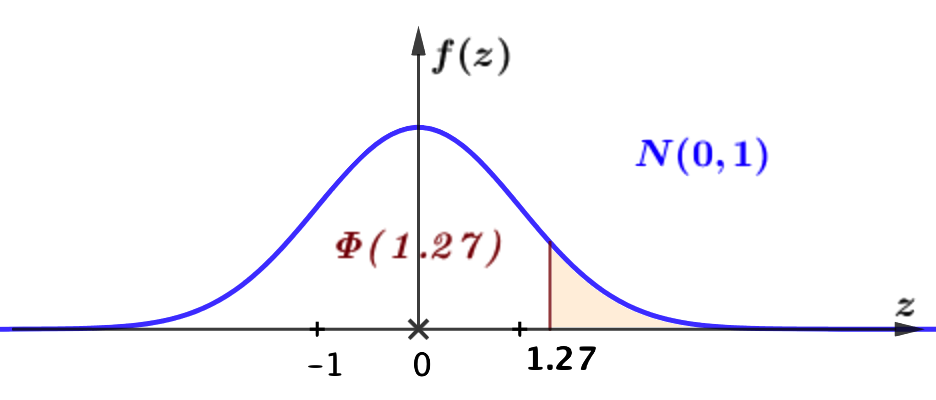
\includegraphics[width=.5\textwidth]{imagenes/imagenes04/T04IM19.png}
	\end{figure}
 	
 \end{multicols}
 

 $c)\ \ p(z\le -0.36)=1-\Phi(0.36)=1-0.640576=0.359424$
 
 
 \begin{figure}[H]
	\centering
	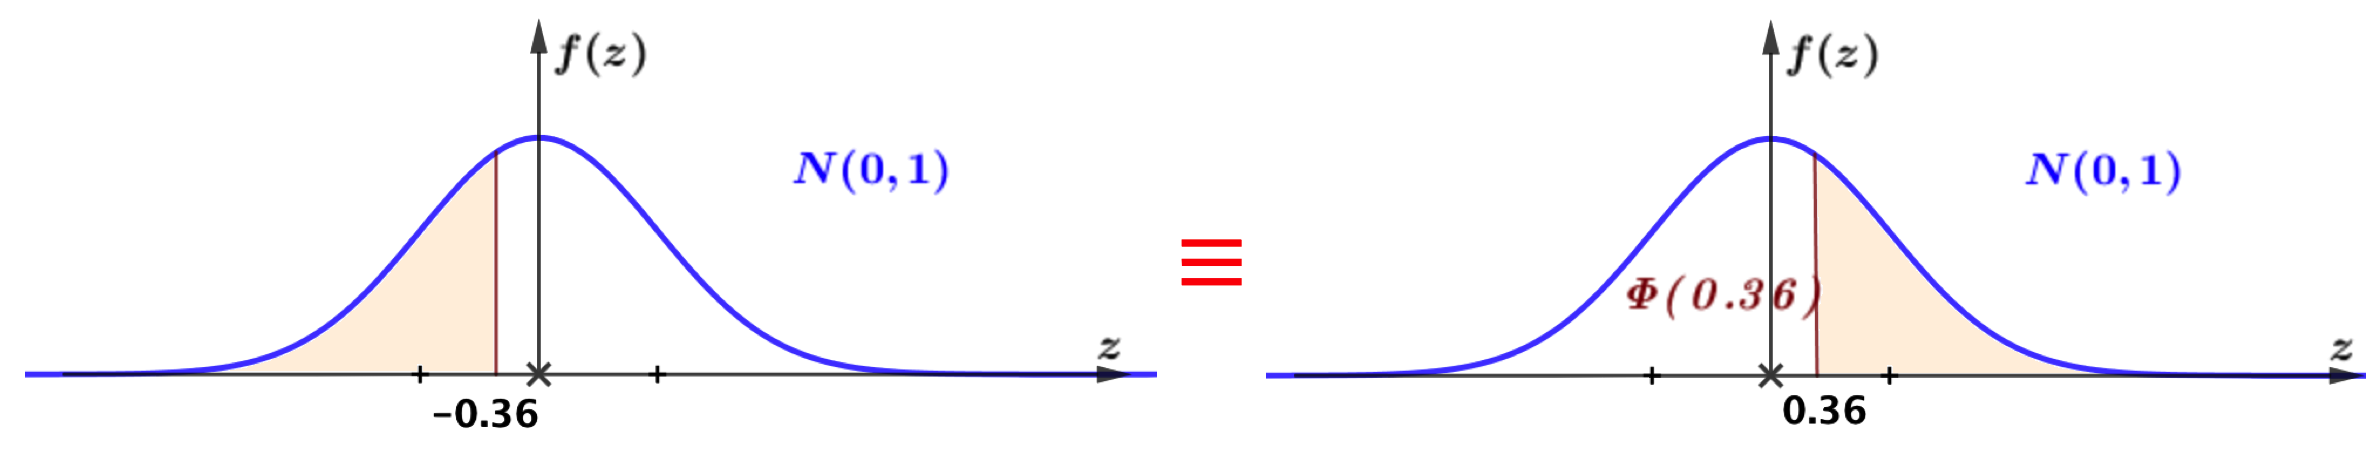
\includegraphics[width=1\textwidth]{imagenes/imagenes04/T04IM20.png}
	\end{figure}
 	

 
 $d)\ \ p(z>-2.75)=\Phi(2.75)=0.997029$
 
 \begin{figure}[H]
	\centering
	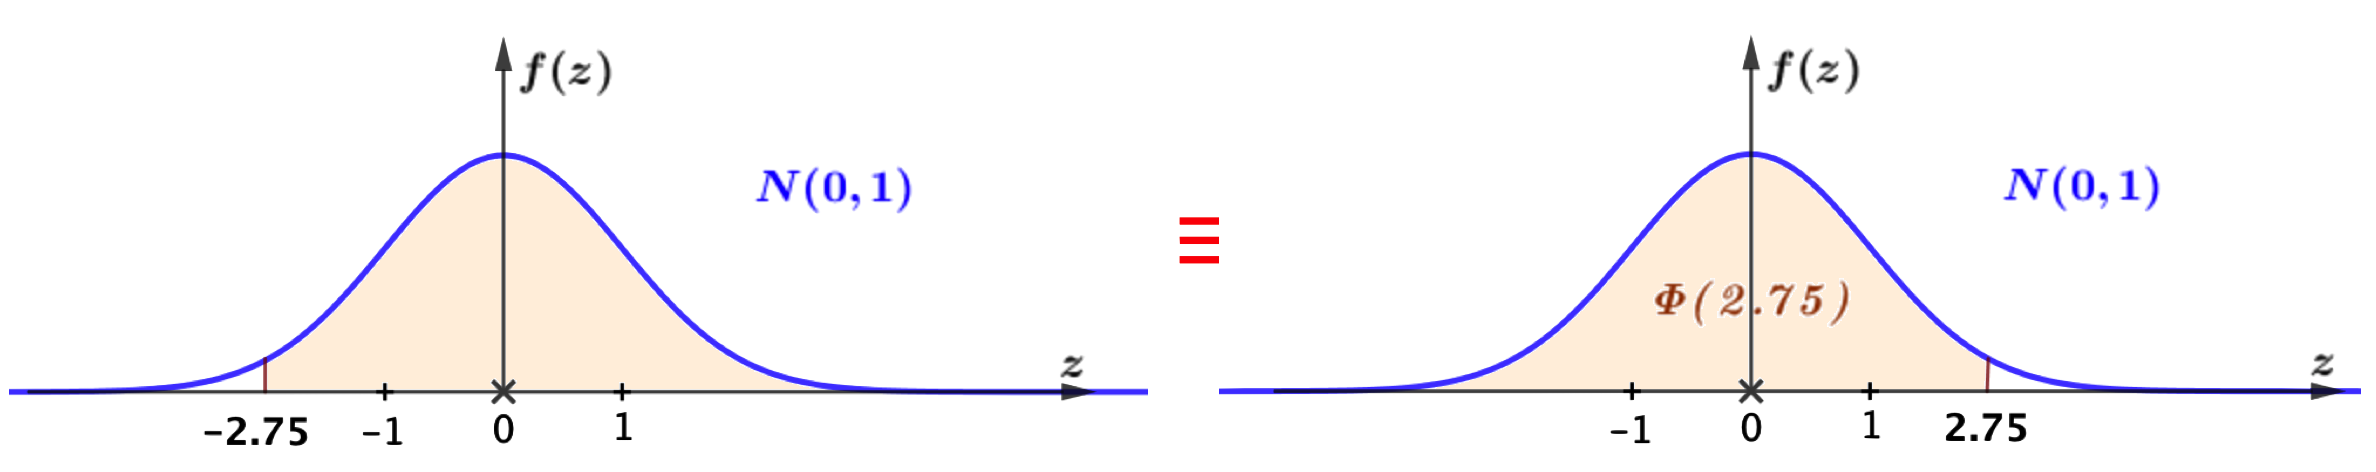
\includegraphics[width=1\textwidth]{imagenes/imagenes04/T04IM21.png}
	\end{figure}
 	
 $e)\ \ p(0.23<z<2.17)=\Phi(2.17)-\Phi(0.23)=0.984997-0.590954=0.394043$

 \begin{figure}[H]
	\centering
	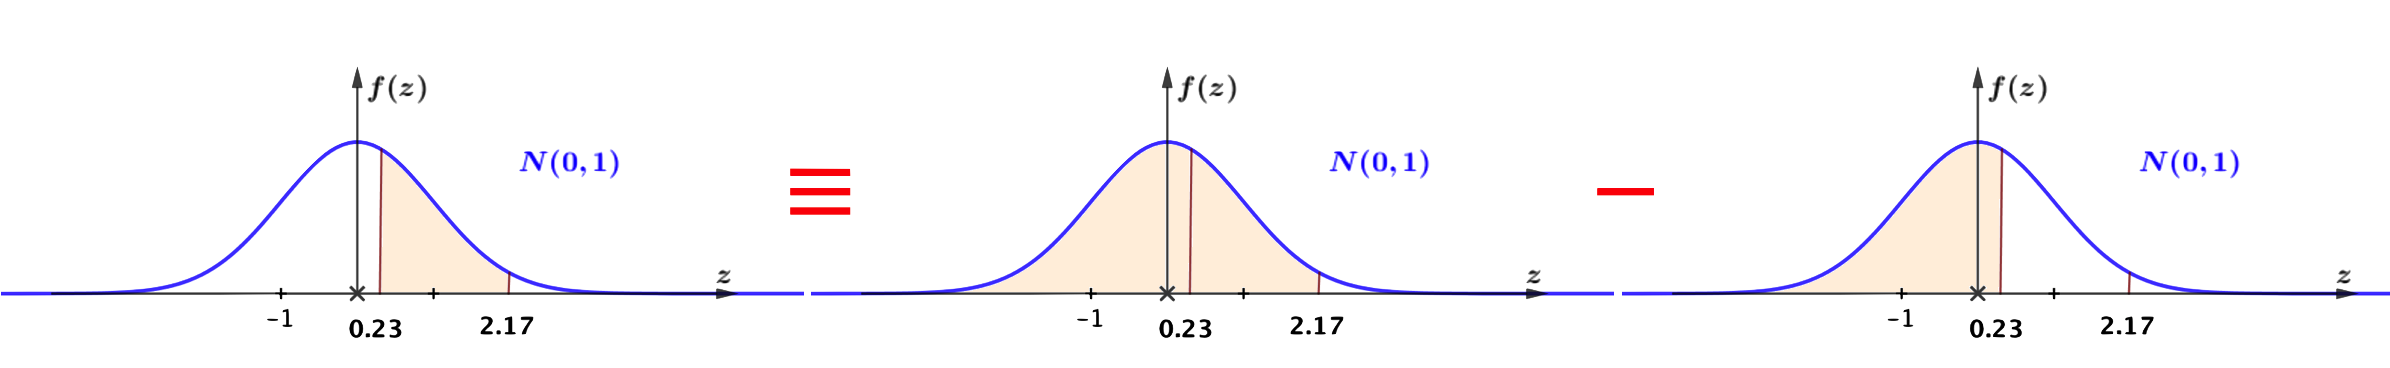
\includegraphics[width=1\textwidth]{imagenes/imagenes04/T04IM22.png}
	\end{figure}
	
$f)\ \ p(-1.74<z<-0.42)=\Phi(1.74)-\Phi(0.42)=0.959070-0.662757=0.296313$	
	\begin{figure}[H]
	\centering
	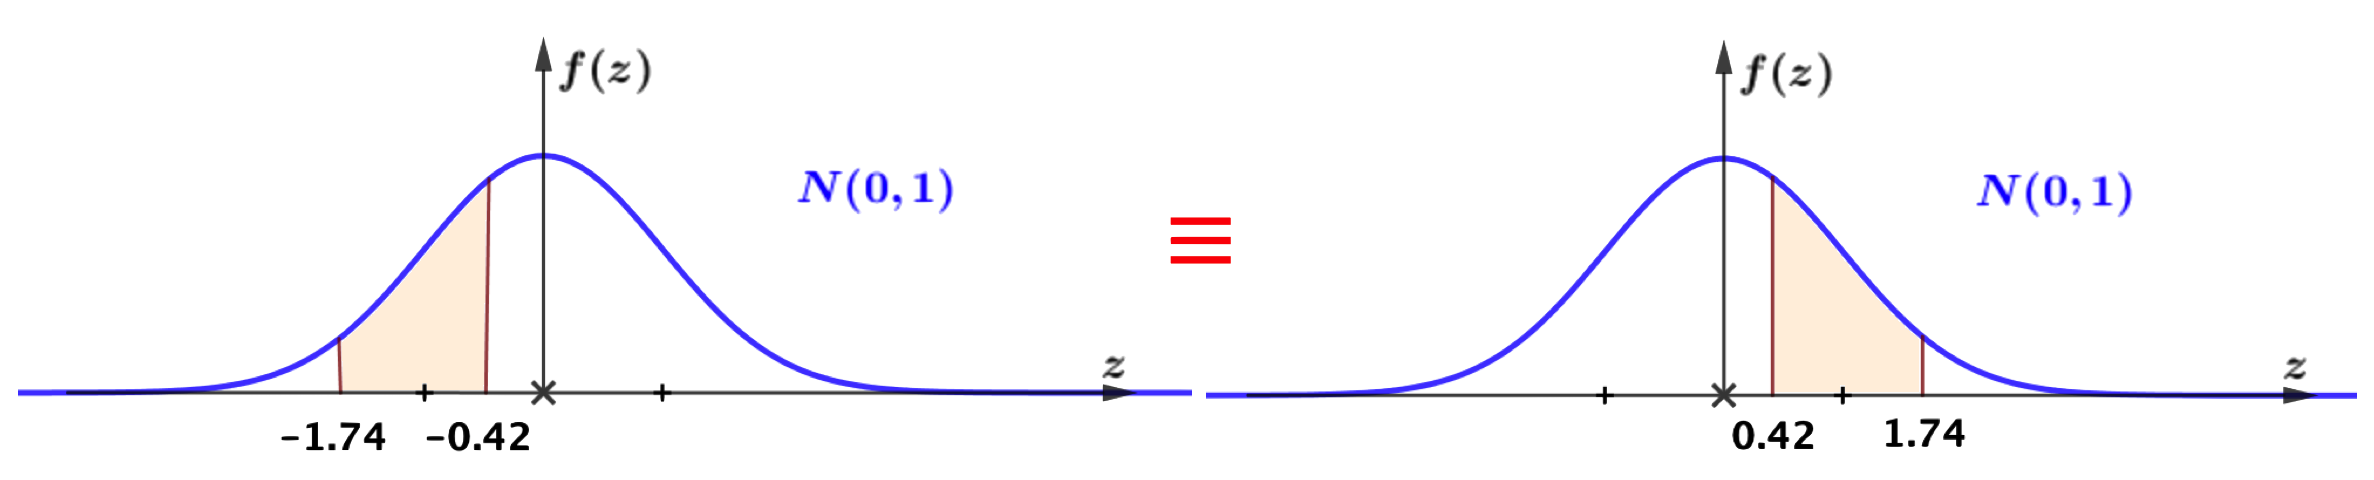
\includegraphics[width=1\textwidth]{imagenes/imagenes04/T04IM23.png}
	\end{figure}
	
	$g)\ \ p(-1.42<z\le 1.00)=\Phi(1)-[1-\Phi(1.42)]=0.841345-[1-0.922196]=0.763541$
	
	\begin{figure}[H]
	\centering
	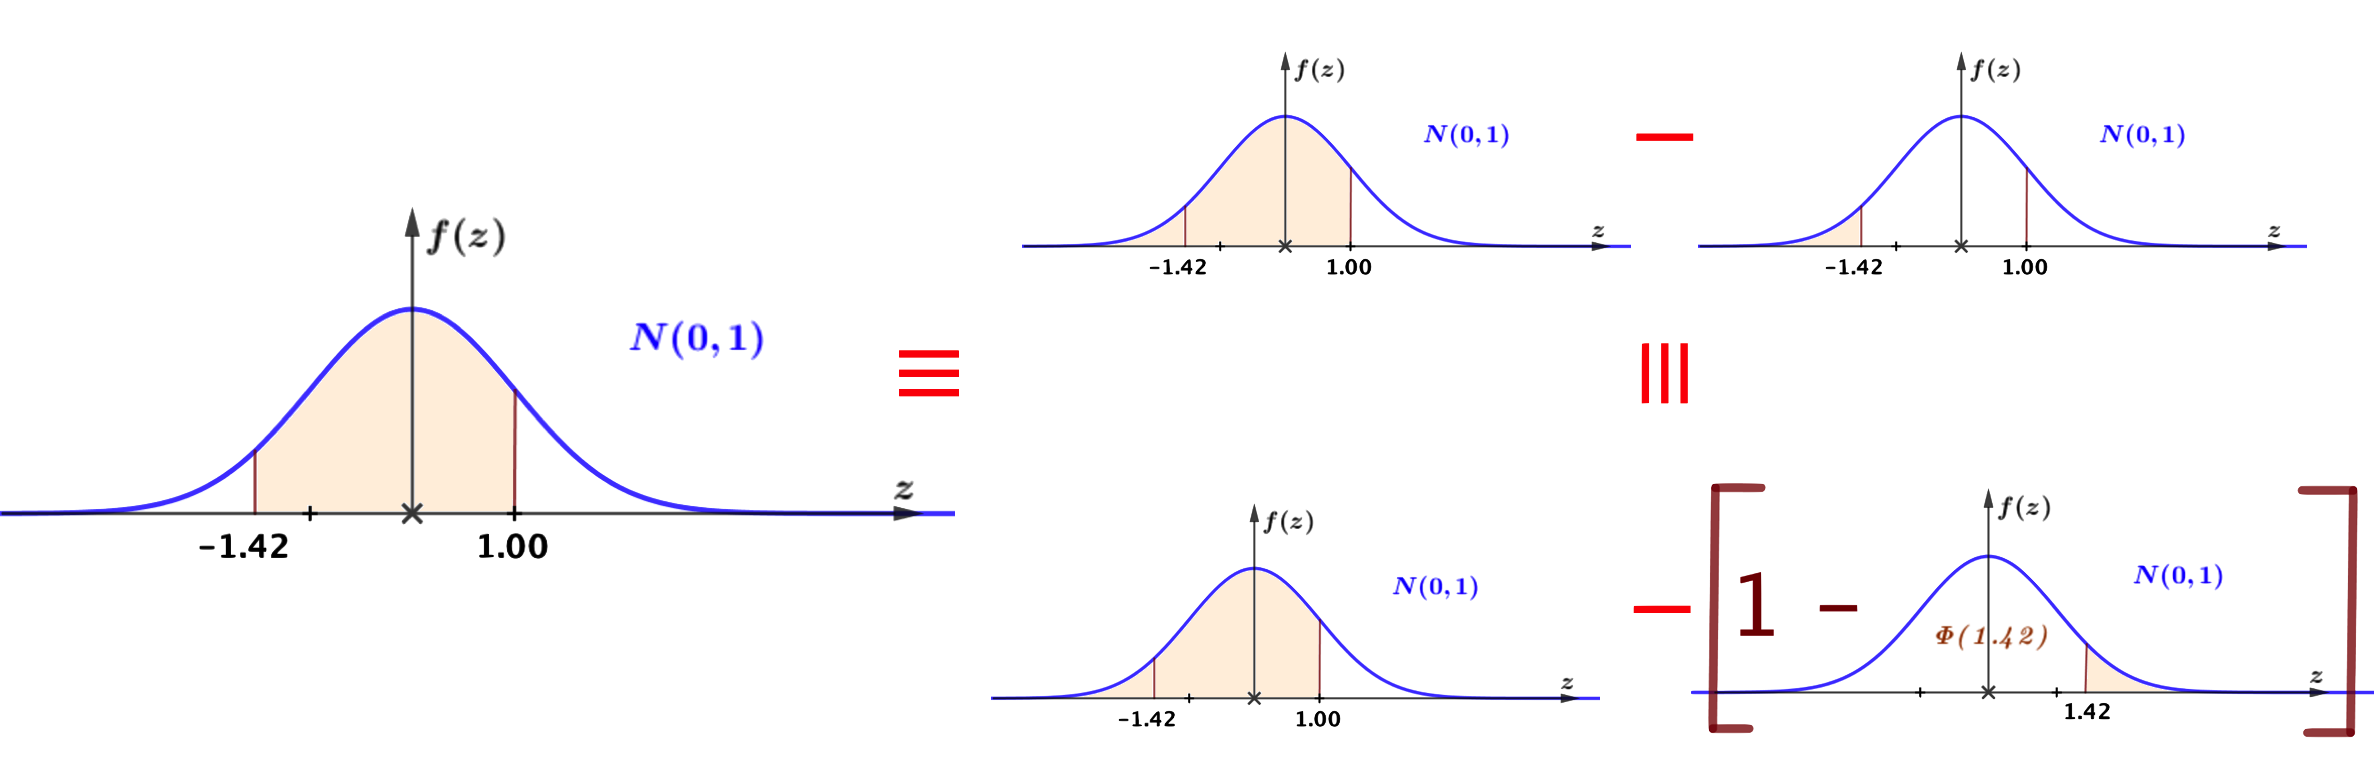
\includegraphics[width=1\textwidth]{imagenes/imagenes04/T04IM24.png}
	\end{figure}
	
\end{ejre}
\end{ejemplo}


\vspace{10mm} %********************************************
\textbf{Cálculo del valor de z a partir de su probabilidad asociada, uso de la tabla en sentido inverso.}

La tabla normal se emplea también en sentido contrario para hallar la abscisa (el valor de $z$) correspondiente a una probabilidad determinada.  Esto es, igual que se sabe que $P(z< 1) = 0.8413$, en sentido contrario la pregunta sería:  ?`Cuánto debe valer $z$ para que $P(z<k)=0.8413$? La respuesta es evidente: el valor debe ser $k=1$.

Si el valor de probabilidad no figura en la tabla tomaremos el más cercano. 
También se puede  interpolar. Así, para $p(z<k)=99.5\%=0.9950$,  tomaremos $z = 2.575$, intermedio entre $2.57$ y $2.58$, con valores de probabilidad respectivos son $0.9949$ y $0.9951$; $k$ es el promedio de los dos valores.


\vspace{10mm} %********************************************
\begin{ejemplo}
\begin{ejre}
Calcula los siguientes valores de $k$ para que:

$a)\ p(z<k)=0.890651;\quad b)\  p(z<k)=0.359424; \quad d)\ p(z>k)=81\%;$

$e)\ p(z>k)=0.15; \ \ \ \qquad f)\ p(-k<z<k)=95\% $

\rule{250pt}{0.1pt}


\begin{multicols}{2}
$a) \ p(z<k)=0.890651>0.5 \to k>0$

Leyendo en la tabla a la inversa: 

\begin{table}[H]
\centering
\begin{tabular}{ccc}
 &  & \textbf{3} \\ \cline{3-3} 
 &  & $\uparrow$ \\
\multicolumn{1}{c|}{\textbf{1.2}} & $\leftarrow $ & 0.890651
\end{tabular}
\end{table}
	
	\begin{figure}[H]
	\centering
	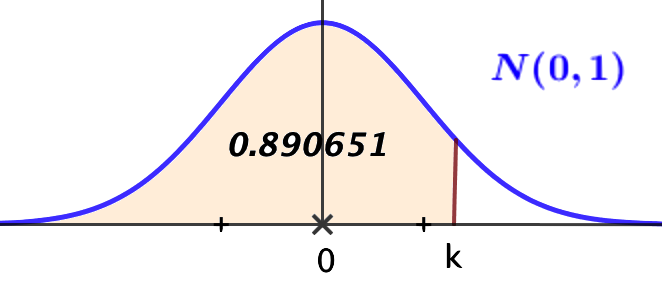
\includegraphics[width=.3\textwidth]{imagenes/imagenes04/T04IM25.png}
	\end{figure}

$\Phi(k)=0.890651 \ \to \ \boldsymbol{ k=1.23 }$
\end{multicols}


\vspace{5mm}
$b)\ p(z<k)=0.359424<0.5 \to k<0$

	\begin{figure}[H]
	\centering
	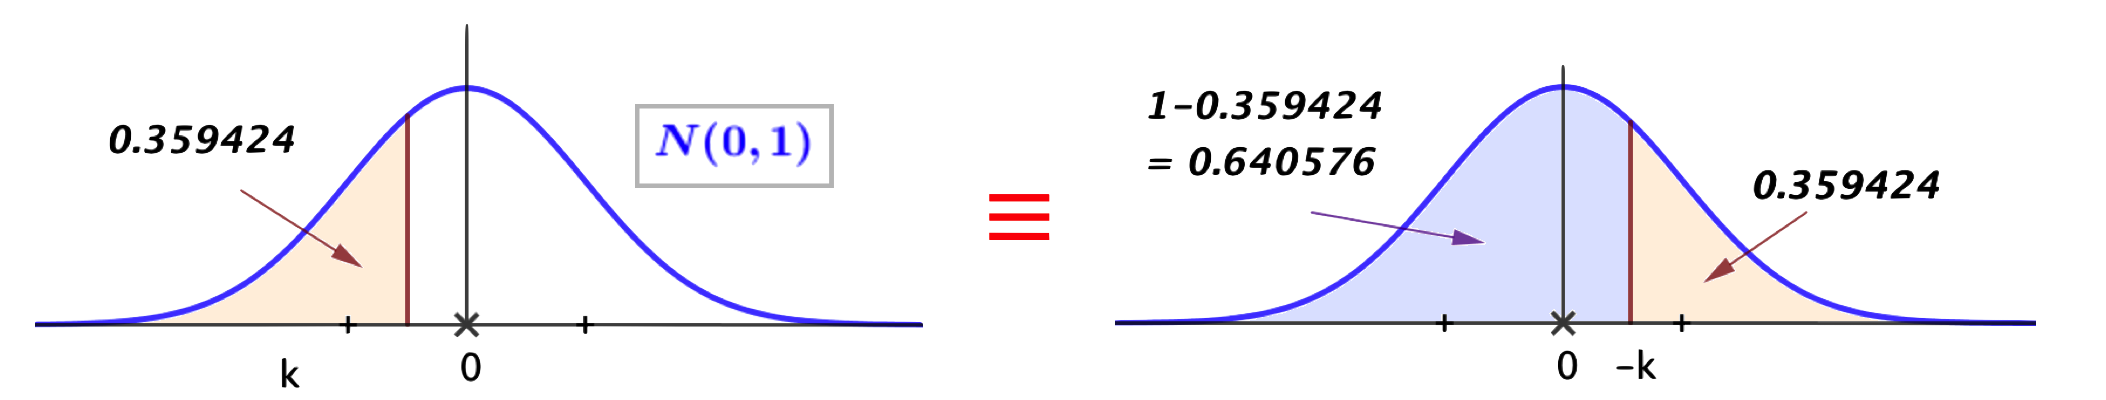
\includegraphics[width=.95\textwidth]{imagenes/imagenes04/T04IM26.png}
	\end{figure}

$\Phi(-k)=1-0.359424=0.640576 \ $ 
\begin{small} \textcolor{gris}{(leyendo la tabla al revés)} \end{small} 
$\to \ -k=0.36 \to \boldsymbol{k=-0.36}$


\vspace{5mm}
$c)\ p(z>k)=81\%=0.810000>0.5 \to k<0$

	\begin{figure}[H]
	\centering
	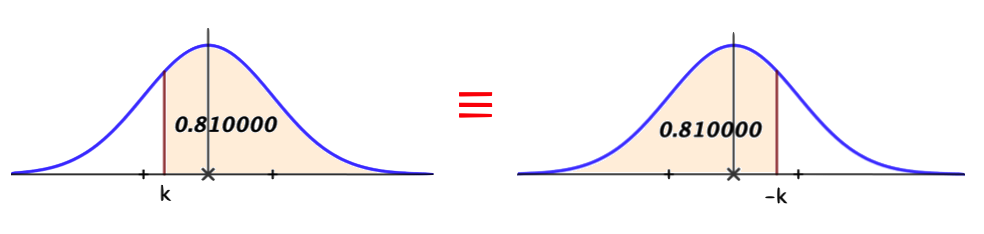
\includegraphics[width=.8\textwidth]{imagenes/imagenes04/T04IM27.png}
	\end{figure}

$\Phi(-k)= 0.810000 \ $ 
\begin{small} \textcolor{gris}{(leyendo la tabla al revés)} \end{small}
$\ \to -k=0.88 \ \to \ \boldsymbol{k=-0.88}$

\vspace{5mm}
$e)\ p(z>k)=0.150000 <0.5 \ \to \ k<0$

	\begin{figure}[H]
	\centering
	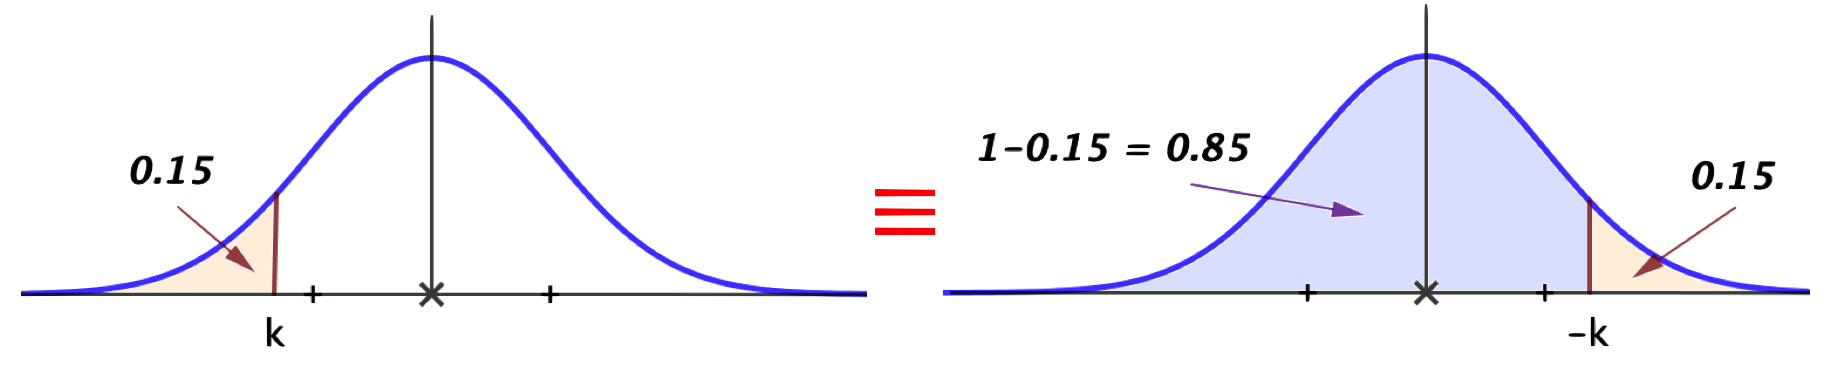
\includegraphics[width=.8\textwidth]{imagenes/imagenes04/T04IM28.png}
	\end{figure}
	
$\Phi(-k)=1-0.15=0.850000\ $
\begin{small} \textcolor{gris}{(leyendo la tabla al revés)} \end{small}
$\ \to -k=1.04 \ \to \ \boldsymbol{k=-1.04}$


\vspace{5mm}
$f)\ p(-k<z<k)=95\%$

	\begin{figure}[H]
	\centering
	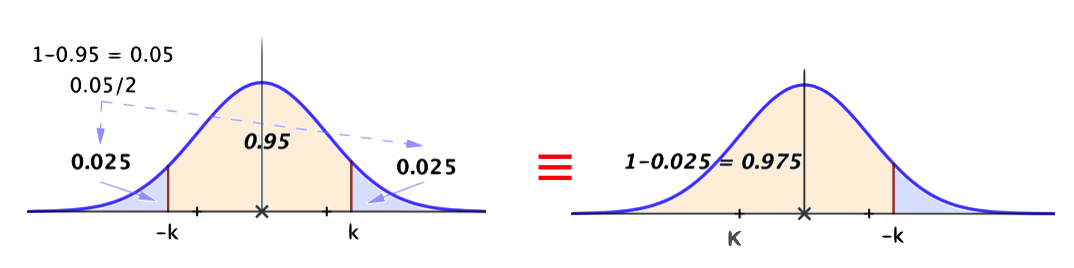
\includegraphics[width=.8\textwidth]{imagenes/imagenes04/T04IM29.png}
	\end{figure}
	
\begin{small} \textcolor{gris}{(leyendo la tabla al revés)} \end{small} $\ \ \Phi(k)=0.975000 \ \to \ \boldsymbol{k=1.96}$

\end{ejre}
\end{ejemplo}


	\begin{figure}[H]
	\centering
	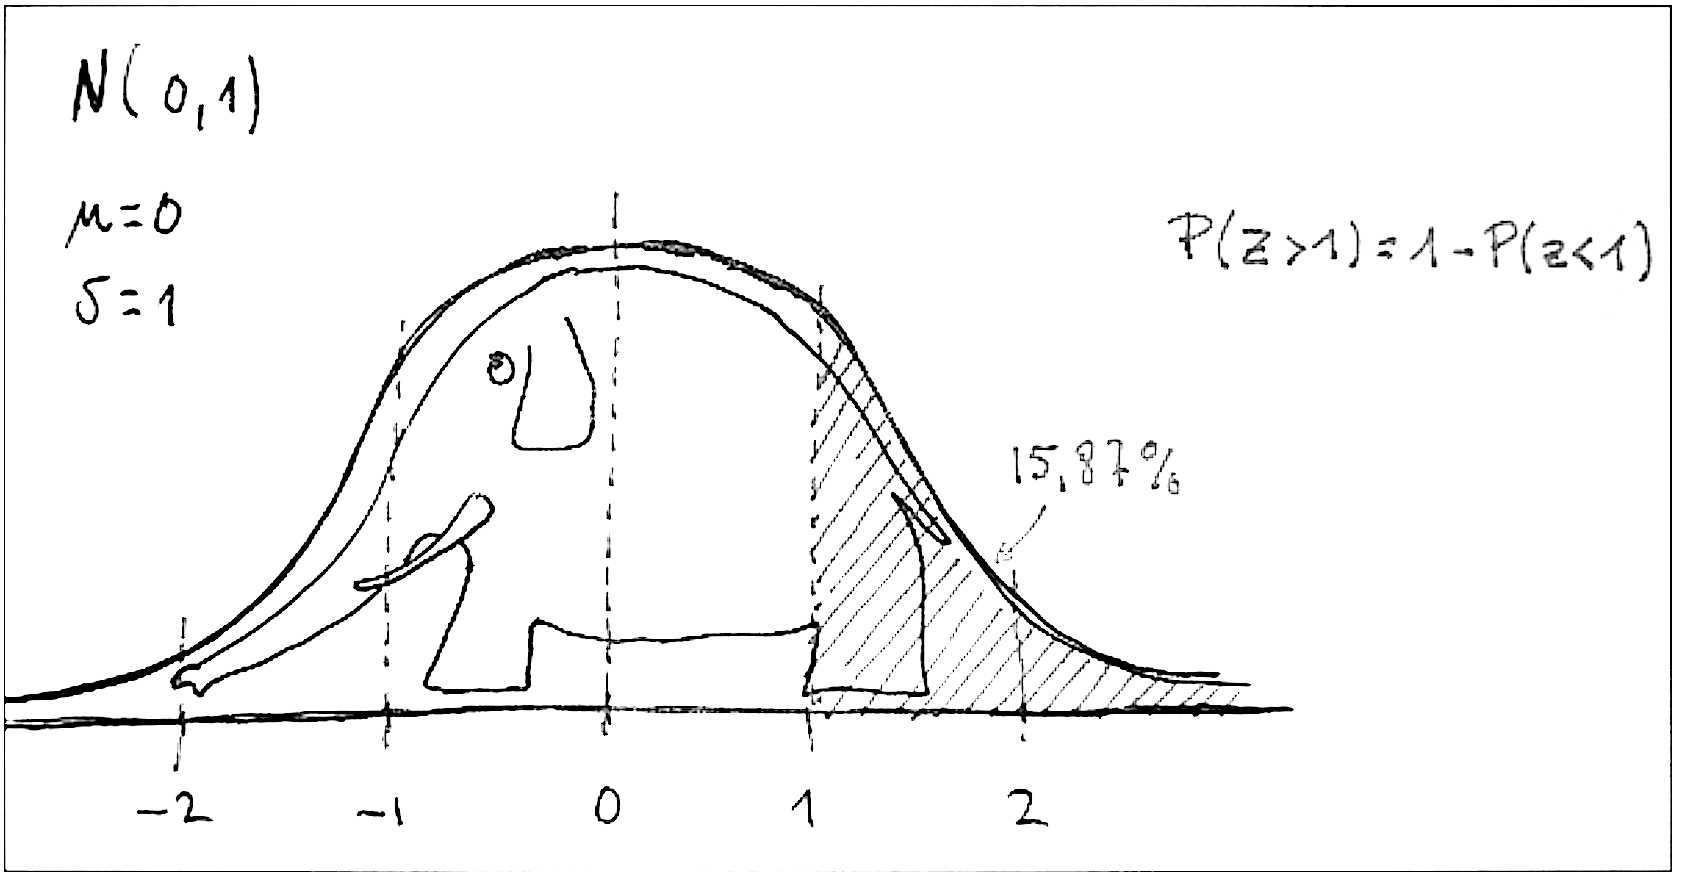
\includegraphics[width=.8\textwidth]{imagenes/imagenes04/T04IM32.png}
	\end{figure}

%\vspace{5mm}
\subsection{Cálculo de probabilidades en una $N(\mu,\sigma)$. Tipificación}



Para poder calcular probabilidades en una $N(\mu,\sigma)$, hemos de transformarla en una $N(0,1)$ de la que disponemos tablas. Para ello necesitamos:

\hspace{1cm} --- trasladar la $N(\mu,\sigma) \ \to \ N(0,\sigma)$

\hspace{1cm} --- contraer/dilatar para que $N(0,\sigma) \ \to N(0,1)$

Todo ello se consigue, de un solo paso, con el siguiente cambio de variable (\emph{tipificación}):

\vspace{5mm}%************************************** 
\begin{definition}
. $$x\in N(\mu,\sigma) \ \to \ z\in N(0,1)\ : \qquad \subrayado{\boxed{\ \boldsymbol{z\ = \ \dfrac{x-\mu}{\sigma}}  \ }}$$

\vspace{2mm} A este cambio de variable se le llama \textbf{tipificación}. Lo usamos pasa pasar de una $N(\mu,\sigma)$ a una $N(0,1)$. 

\vspace{2mm} Con ello: $\quad p(x<k)\ = \ p \left( z<\dfrac {k-\mu}{\sigma} \right) ;\qquad p(x\ge k)\ = \ p \left( z\ge \dfrac {k-\mu}{\sigma} \right);$

\vspace{2mm}$p(k_1\le x<k_2)\ = \ p \left( \dfrac {k_1-\mu}{\sigma} \le z < \dfrac {k_2-\mu}{\sigma} \right) ; \qquad etc $
\end{definition}

\vspace{4mm}%************************************** 
\begin{example}
.	En una $N(7,2.3)$, calcula $p(x<8.45)$

\vspace{2mm} 	$x=8.45 \to z=\dfrac{8.45-7}{2.3}=0.63>0$, leyendo directamente en las tablas, 

$p(x<8.45)=p(z<0.63)=\Phi(0.63)=0.735653\approx 74\%$
\end{example}

\vspace{4mm}%************************************** 
\begin{ejemplo}
\begin{ejre}
	En una $N(50,5)$, calcula: $p(x<56);\ \ p(x>48);\ \ p(48<x<56)$ ?`Cuál es el percentil 75 de esta distribución? 
	
\rule{250pt}{0.1pt}

$$N(50,5) \ \to \ \mu=50;\ \sigma = 5 \ \longrightarrow \ \text{ tipificación: }\ z=\dfrac{x-50}{50} \ \to \ N(0,1)$$

--- $\ p(x<56)=p\left( z<\dfrac{56-50}{5} \right) = p(z<1.2)=\Phi(1.2)=0.884930$

--- $\ p(x<48)= p\left( z<\dfrac{48-50}{5} \right) = p(z<-0.4) $; $\ z<0$, buscamos la situación simétrica:

\begin{multicols}{2}
	
	$p(x<48)=p(z<-0.4)=p(z>0.4)=$
	
	$=1-p(z<0,4)=1-\Phi(0.4)=$
	
	$1-0.655422=0.344578$
	
	\begin{figure}[H]
	\centering
	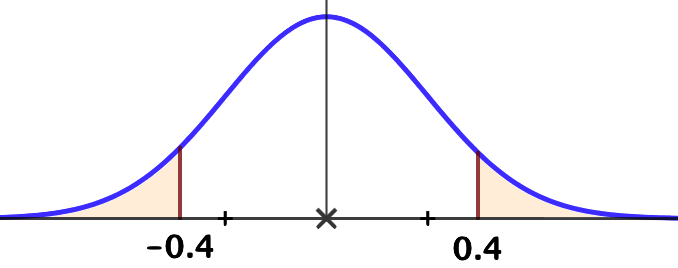
\includegraphics[width=.4\textwidth]{imagenes/imagenes04/T04IM30.png}
	\end{figure}
	
\end{multicols}

--- $\  p(48<x<56)=$\textcolor{gris}{(tipificación)}$=p \left( \dfrac{48-50}{5} <z< \dfrac{56-50}{5} \right) = p(-0.4<z<1.2)$

	\begin{figure}[H]
	\centering
	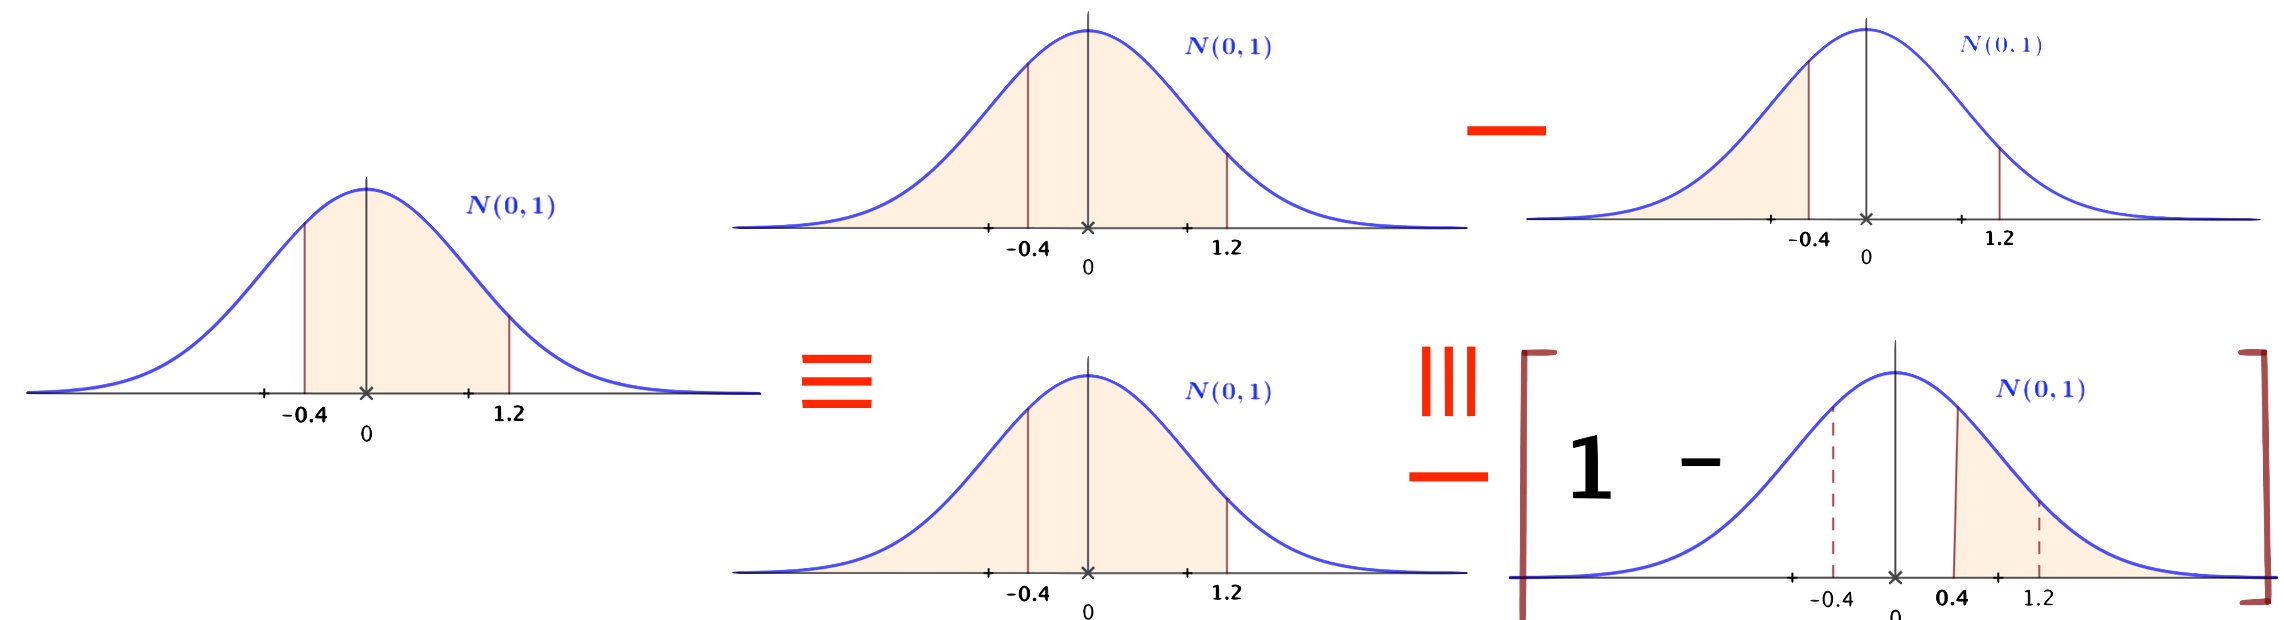
\includegraphics[width=1\textwidth]{imagenes/imagenes04/T04IM34.png}
	\end{figure}
	
$\  p(48<x<56) = p(-0.4<z<1.2) = \Phi(1.4)-[ \ 1-\phi(0.4) \ ]= 0.884930-[1-0.655422]=0.540352$

--- Percentil 75: $\ P_{75}= k \leftrightarrow P(x<k)=p \left( z<\dfrac{k-50}{5} \right) =0.75=0.750000 \to $ \textcolor{gris} (leyendo las tablas al reves) $\to P_{75}:\ \ \dfrac{k-50}{5}=0.675 \to P_{75}=k=53.375$
\end{ejre}	
\end{ejemplo}

\vspace{4mm}%************************************** 
\begin{ejemplo}
\begin{ejre}
	Las alturas de 800 estudiantes se distribuyen normalmente con media 173 cm y desviación típica 11 cm. Aproximadamente, ?`cuántos alumnos tienen una altura)
	
	a) De 175 cm; b) menor a 175 cm; c) entre 175 y 190 cm; d) ?`qué altura hay que tener para estar entre los 10\% más altos?

\rule{250pt}{0.1pt}

--- $a)\ p(x=175)=0\ $ La probabilidad de que una v.a. continua tome un valor concreto es cero.

--- $b)\ p(x<175)=p \left( z<\dfrac{175-173}{11} \right) = p(z<0.18)=\Phi(0.18)=0.571424$

Del total de los $800$ alumnos, $800\cdot 0.571424\approx 457 \ $ de ellos miden menos de $175 \ \mathrm{cm}$ .

--- $ c) \ p(175<x<190)=p\left( \dfrac{175-173}{11}<z<\dfrac{190-173}{11} \right)=p(0.18<z<1.55)=\Phi(1.55)-\Phi(0.18)=0.939429-0.571424=0.368005$

Del total de los $800$ alumnos, $800 \cdot 0.368005\approx 294$ de ellos tienen alturas comprendidas entre $175 \text{  y } 190 \ \mathrm{cm}$.

--- Estar entre el 10\% de los más altos es lo mismo que dejar por detrás, en altura, al 90\% de los alumnos del centro; es decir, estar en el percentil 90: $P_{90}=k \leftrightarrow p(x<k)=90\%$

$p(x<k)=p\left(z< \dfrac{k-173}{11} \right) =0.900000 \to $ \textcolor{gris} (leyendo las tablas al revés) $\to \dfrac{k-173}{11}=1.28 \Rightarrow k=187.1 \mathrm{cm}=P_{90}$ Para estar entre el 10\% de los más altos de ese centro hay que medir más de $187.1 \mathrm{cm}$.

\end{ejre}	
\end{ejemplo}

\vspace{4mm}%************************************** 
\begin{ejemplo}
\begin{ejre}
	En una determinada ciudad, sus habitantes se distribuyen, en edades, como una media de 40 años. Se sabe que el 3,35\% de los habitantes de esa ciudad tienen más de 60 años.
	
	?`Cuál es la desviación típica? ?`Qué porcentaje de la población es menor de 25 años?
	
\rule{250pt}{0.1pt}

$a)\ \ p(x>60)=p\left( z> \dfrac{60-40}{\sigma} \right) =0.0335 $ \textcolor{gris} (leyendo las tablas al revés) $\dfrac{20}{\sigma}=1.835 \to \boldsymbol {\sigma=10.9}$

$b)\ \ $ En una $N(40,10.9)$, $\ p(x<25)=p \left( z<\dfrac {25-40}{10-9} \right) = p(z<-1.38)= $\textcolor{gris} (simetría) =$p(z>1.38) = 1-\Phi(1.38)=1-0.916207=0.083793 \approx 8.37\%$
\end{ejre}	
\end{ejemplo}


\vspace{5mm} %***************************
\section{Aproximación de la Binomial por una Normal}

\begin{theorem}

	El \textbf{Teorema central del límite} dice que si $X_,X_2,\cdots, X_n$ son $n$ v-a. independientes con medias $\mu_1, \mu_2, \cdots, \mu_n$ y desviaciones típicas $\sigma_1, \sigma_2,\cdots,\sigma_n$, entonces, la variable $Y=X_1+X_2+\cdots +X_n$, ``cuando \textbf{$\boldsymbol{n}$ es gramde}'',  se aproxima a una distribución \textbf{normal} con media $\mu_1+ \mu_2+ \cdots+ \mu_n$ y desviación típica $\sqrt{\sigma_1^2+\sigma_2^2+ \cdots + \sigma_n^2}$

\begin{small} $$ \boldsymbol{ Y=X_1+X_2+\cdots +X_n \ \longrightarrow \ N \left(\ \mu_1+ \mu_2+ \cdots+ \mu_n\ ,\ \sqrt{\sigma_1^2+\sigma_2^2+ \cdots + \sigma_n^2} \ \right) }$$ \end{small}

\end{theorem}

\vspace{4mm} %******************

\begin{theorem}

\textbf{Aproximación de la binomial a la normal}	

\begin{multicols}{2}
Por el teorema central de límite (anterior), podremos considerar una variable $X$ que siga una distribución binomial $B(n, p)$, como una suma de $n$ variables  independientes $X_i$ con media $p$ y varianza $p(1-p)$, pues suponemos que $X_i$ toma el valor uno si el ensayo es un éxito, y toma el valor cero si es un fracaso, es decir:

\begin{table}[H]
\centering
\begin{tabular}{c|c|c|c|}
\hline
\multicolumn{1}{|c|}{\textbf{$x_i$}} & \textbf{$p_i$} & \textbf{$x_i\ p_i $} & \textbf{$x_i^2\ p_i$} \\ \hline
\multicolumn{1}{|c|}{1} & p & p & p \\ \hline
\multicolumn{1}{|c|}{0} & 1-p & 0 & 0 \\ \hline
$\Sigma$ & \textbf{1} & \textbf{p} & \textbf{p} \\ \cline{2-4} 
\end{tabular}
\end{table}
\end{multicols}

Calculamos la media y la desviación típica:

$\mu=\displaystyle \sum_{i=1}^2 \ x_i\ p_i=1\ p + 0 \ (1-p)=0;$

$\displaystyle \sigma^2= \sum_{i=1}^2 x_i^2\ p_i - \mu^2=1^2 \ p+ 0^2 \ (1-p) \ - \ p^2=p-p^2=p(1-p)=p\ q$

\vspace{2mm} Por tanto, como consecuencia del teorema central del límite, y si $n$ es grande, podemos aproximar una variable aleatoria $X$ que siga una distribución binomial $B(n,p)$ por una distribución normal cuya media y desviación típica son:

\vspace{2mm} $\mu=\mu_1+\mu_2+\cdots +\mu_n=p+p+\cancelto{n-veces}{ \cdots} +p=n\ p$

\vspace{2mm} $\sqrt{\sigma_1^2+\sigma_2^2+ \cdots + \sigma_n^2} = \sqrt{pq+pq+\cancelto{n-veces}{ \cdots} +pq }=\sqrt{ n\ p\ q}$

\vspace{2mm}
$$\subrayado{\ \boxed{  \boldsymbol{X\leadsto B(n,p) \ \ n\ \textbf{ ``grande`` } \ \ \to \ \ X \leadsto N(\ \mu=np\ ,\ \sigma=\sqrt{npq}\ )} \ } \ }$$

\end{theorem}

\vspace{4mm} %******************
\begin{myalertblock}
	{Validez de la aproximación de la binomial a la normal}
	
Abraham de Moivre demostró que esta aproximación es buena si $n$ es mayor que $30$ y $p$ no está próximo a cero ni a uno. En general se considera que la aproximación es buena si:


$$\boldsymbol{
B(n,p) \approx N(np,\sqrt{npq} \ \ \text{ si } \ \ n	\ge 30 \ \wedge \  np \ge 5  \ \wedge \  n(1-p) \ge 5
}$$

Si no se cumplen estas condiciones NO se puede se puede usar la aproximación.
\end{myalertblock}

\begin{figure}[H]
	\centering
	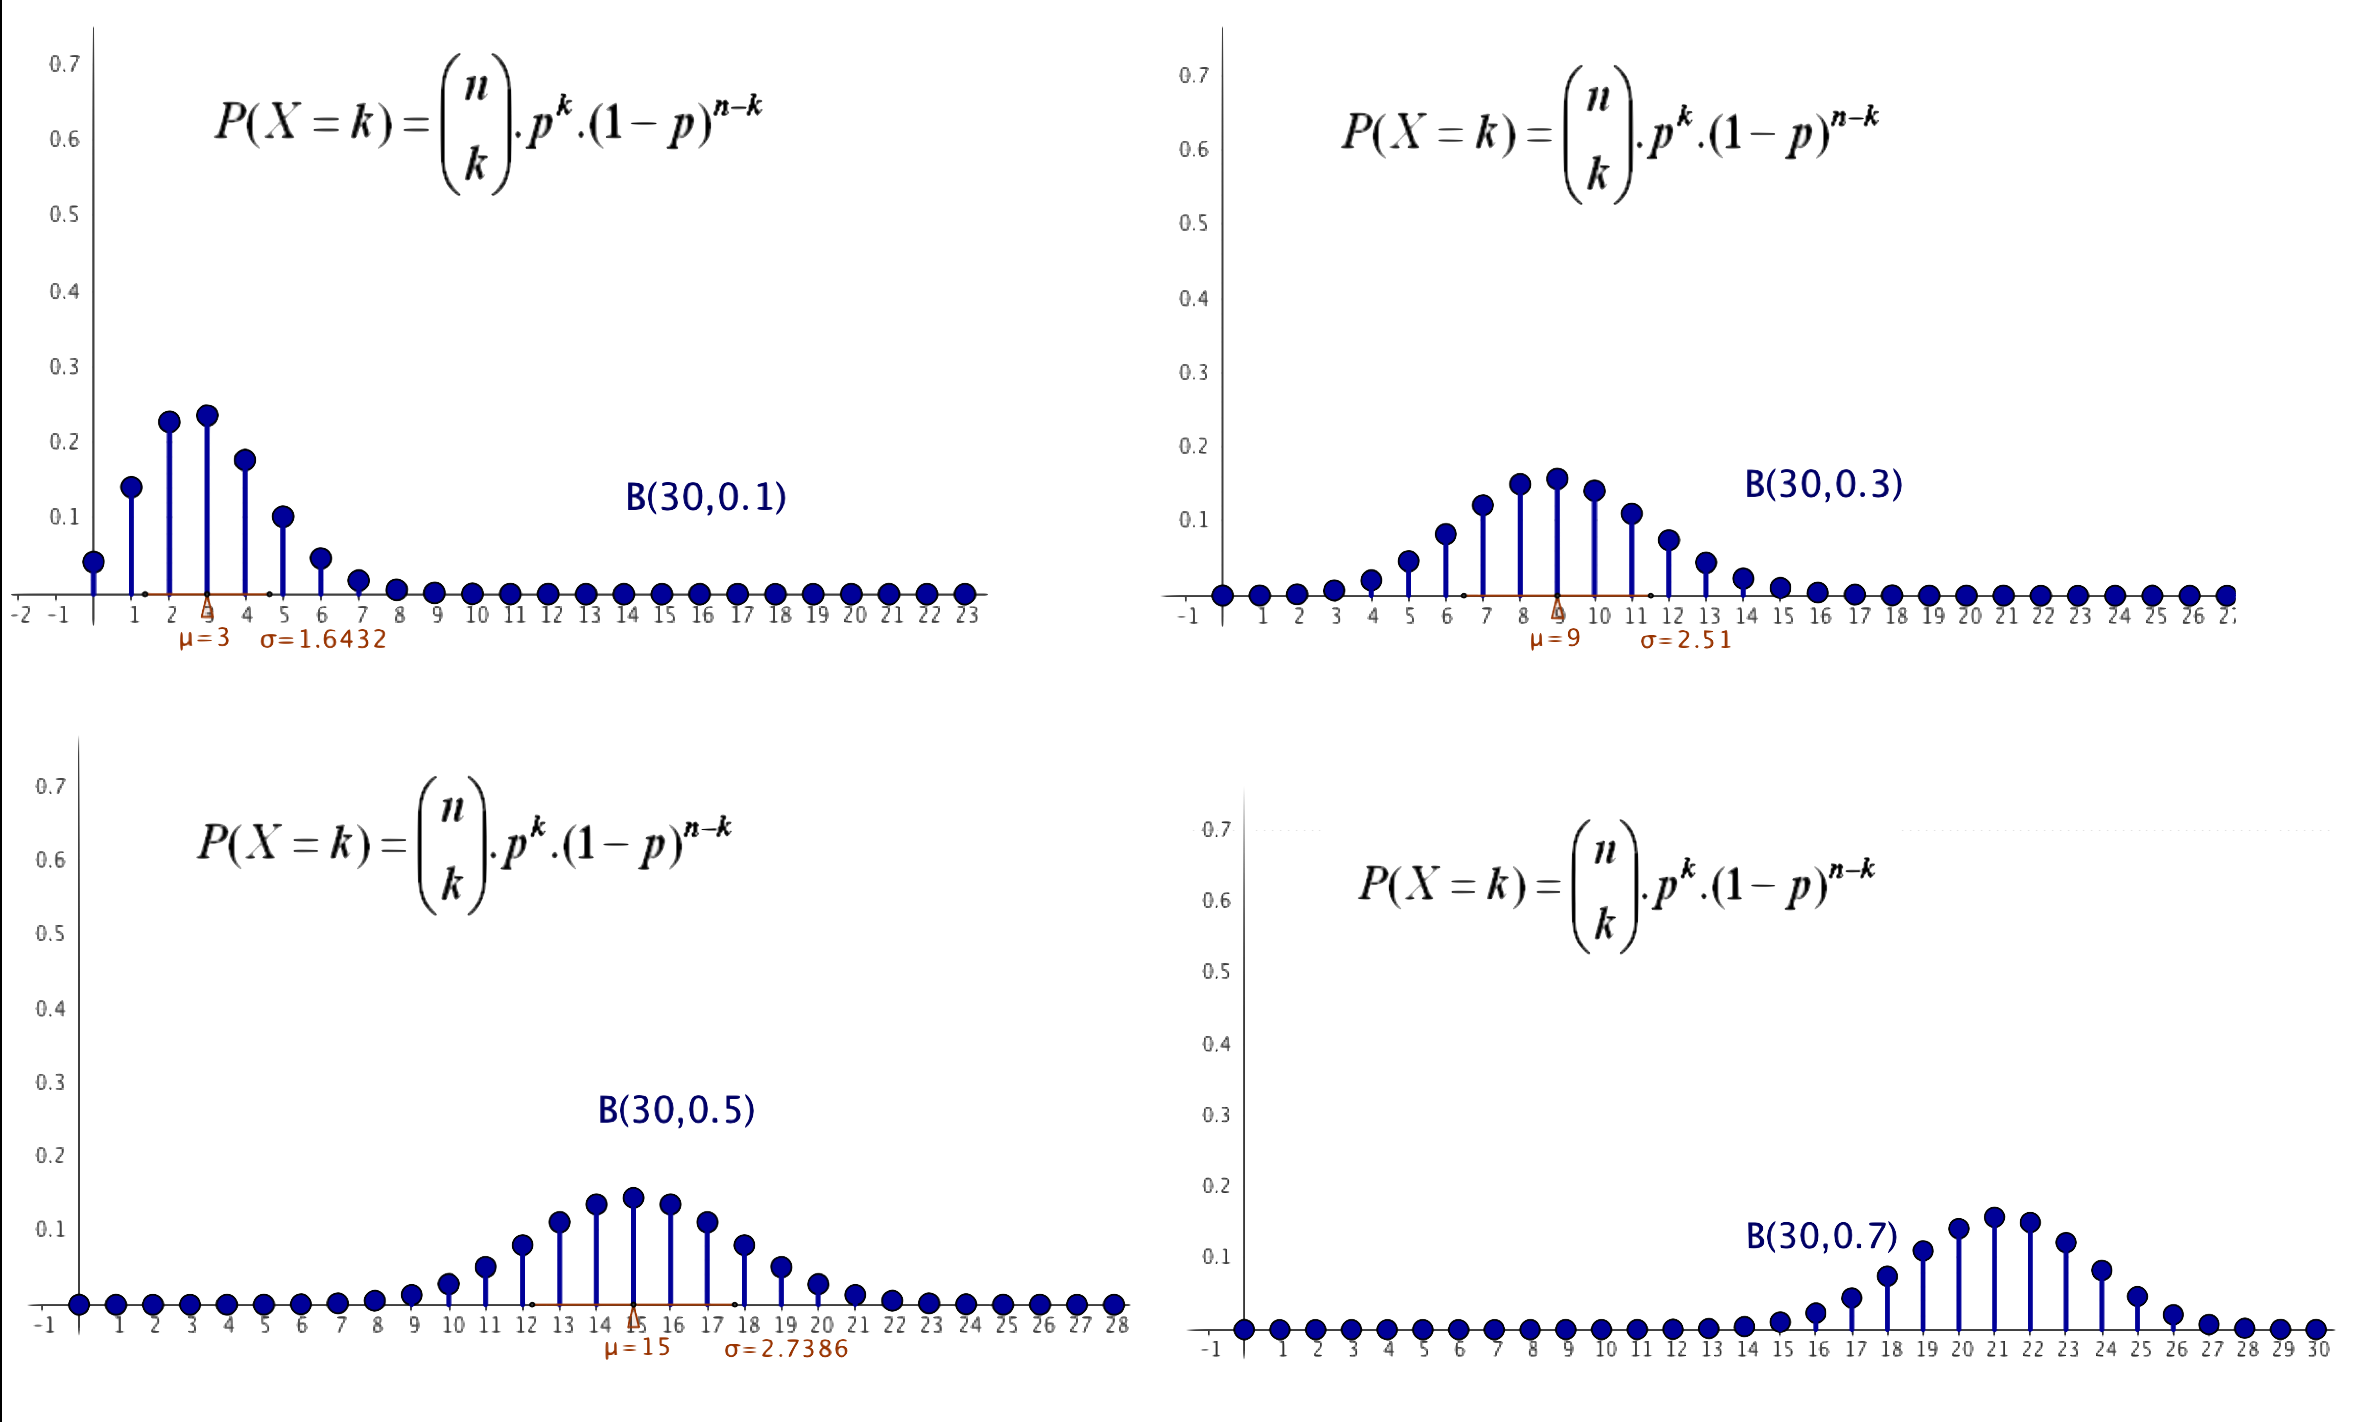
\includegraphics[width=1\textwidth]{imagenes/imagenes04/T04IM39.png}
	\end{figure}

\vspace{4mm} %******************
\begin{destacado}

En el caso de que podamos aproximar la Binomial por una Normal, hemos de tener en cuenta que estamos pasando de una variable discreta (binomial), X, a una variable continua (normal), que llamaremos X' y es necesario efectuar una \textbf{\emph{``corrección por continuidad''}} \textcolor{gris}{$\ $(Como $p(x=k)$ sí tiene sentido en v.a. discreta pero no en continua, $p(x'=k)=0$, cuando hagamos la aproximación $B\approx N$ tomaremos para $k$ el intervalo $x'\in ]k-0.5,k+0.5[\ $)}

\end{destacado}

\vspace{4mm} %******************
Al igual que llamábamos $x$ a la v.a. normal y $z$ a la v.a. normal tipificada, ahora también haremos una distinción entre los nombres que damos a las variables: si $x$ es la v.a. discreta, cuando aproximemos por una distribución de probabilidad de v.a. continua usaremos la variable $\boldsymbol { x' } $.

\vspace{4mm} %******************
\begin{myalertblock}{Corrección por continuidad}
	
Es importante tener en cuenta que en el caso continuo la probabilidad asociada a un valor concreto de la variable es nula, 
$p(x=k)=0$, por tanto, cuando se aproxima una distribución discreta (x') a una distribución normal (x), 
que es continua, se debe utilizar la \textbf{corrección de continuidad} de Fisher o corrección de medio intervalo. 
Esta corrección consiste en considerar cada valor discreto $x'$ como un intervalo de amplitud $1$ de la forma $[x-0.5,x+0.5]$. Así pues:


\begin{itemize}
\item $p(x=k)=p(k-0.5<x'<k+0.5)$  
\item $p(x\le k)=p(x'<0+0.5)$ \begin{footnotesize} (tomamos el valor de k) \end{footnotesize} 
\item $p(x<k)=p(x'<x-0.5)$ \begin{footnotesize} (no tomamos el valor de k) \end{footnotesize}
\item $p(x\ge k)=p(x'\ge x-0.5)$	 \begin{footnotesize} (tomamos el valor de k) \end{footnotesize}
\item $p(x>k)=p(x'>k+0.5)$ \begin{footnotesize} (n0 tomamos el valor de k) \end{footnotesize}

\item  \begin{footnotesize} $p(k_1 < x < k_2)=p(k_1 + 0.5< x' < k_2-0.5); \ \ p(k_1< x \le k_2)= p(k_1+0.5 < x'<x+0.5);\ \ etc$ \end{footnotesize}
\end{itemize}

	\begin{figure}[H]
	\centering
	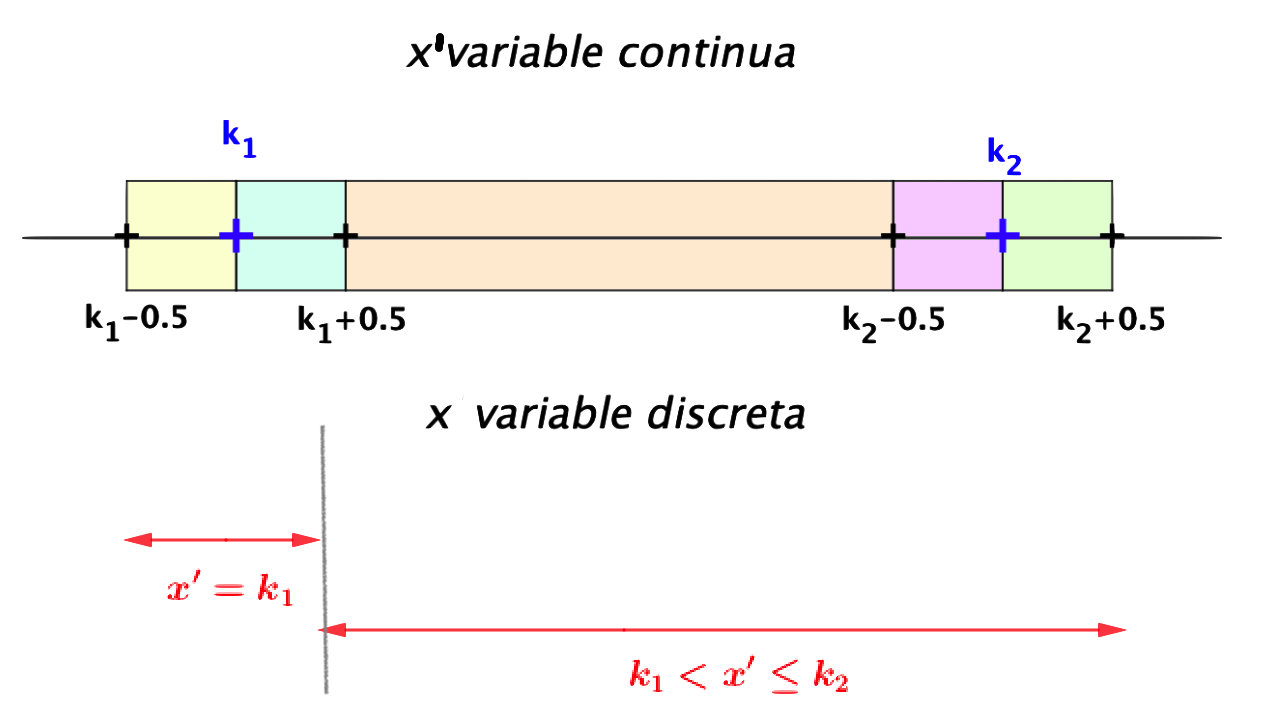
\includegraphics[width=.9\textwidth]{imagenes/imagenes04/T04IM35.png}
	\end{figure}
	
\end{myalertblock}

\vspace{10mm}%**************************
\begin{destacado}
	

	
 $$\ \ \boldsymbol{
B(n,p) \approx N(np,\sqrt{npq}) \ \ \text{ si } \ \ n	\ge 30 \ \wedge \  np \ge 5  \ \wedge \  n(1-p) \ge 5
}$$

	$$\boxed{ \ \  \boldsymbol{ x\in  B(n,p) \  \leadsto \ x'\in N(\mu,\sigma) \ \leadsto \ z\in N(0,1)}  \ \ }$$

\begin{small}	
En la aproximación $B\approx N$, $\ 1^o)\ $ `corrección por continuidad' y $2^o)\ $ `tipificación de la variable'. 
\end{small}
	
\end{destacado}



\vspace{4mm}%**************************
\begin{example}

Es un hecho comprobado que cuando tenemos una distribución binomial $B(n;p)$, a medida que $n$ crece, es difícil hacer uso de las fórmulas y/o tablas.

\vspace{2mm} Por ejemplo, si tiramos un dado 500 veces, calcular la probabilidad de obtener entre 100 y 165 cincos (ambos inclusive).

\vspace{2mm} Llamamos   `éxito = obtener cinco' entonces $p = 1/6$ y `fracaso = no obtener cinco' y $q = 5/6$.

\vspace{2mm} Tenemos una $B (500; 1/6)$ , y nos piden $p(100 \le x \le 165)$.

\vspace{2mm} Es inviable aplicar las tablas (pues repetimos el experimento 500 veces) y tampoco las fórmulas pues habría que hacer 65 cálculos difíciles, del tipo 
  $\ p(x=137)=\mqty(500\\137)(1/6)^{137}(5/6)^{363}$
  
  
  \vspace{2mm} Afortunadamente, como
   $ n \ge  3 0 , \ n p = 83.33 \ge  5 \text { y }  n q  = 8. 3  3 \ge  5$ , se puede aproximar la binomial por una normal: 
   
   $\mu=np=83.33;\ \sigma=\sqrt{npq}=8.33 \ \to X \in B(500,1/6) \ \approx \ X'\in N(83.33,8.33)$
   
  \vspace{2mm}  Así, $\ p(100\le x \le 165)= $ \textcolor{gris}{(corrección por continuidad)} $ = p(100-0.5\le x' \le 165+0.5) =$ \textcolor{gris}{(tipificación)} $=p \left( \dfrac{99.5-83.33}{8.33} < z < \dfrac{165.5-83.33}{8.33} \right) = p( 1.94<z< 9.86)= \Phi(9.86)-\Phi(1.94)= $ \textcolor{gris}{(con la precisión de las tablas que tenemos)} $=1-0.973810=0.02619$

\end{example}	
	


\vspace{4mm}%**************************
\begin{ejemplo}
\begin{ejre}
Una moneda se lanza $400$ veces. Calcula la probabilidad de que el número de caras:
a) Sea mayor que $200$; b) Esté entre $180$ y $220$, ambos inclusive.

\rule{150pt}{0.1pt}

Llamando `éxito' al obtener cara al lanzar la moneda, $p=q=0.5$ y realizamos el experimento  $n=400$ veces. Tenemos una $B(400,0.5)$

--- $a)\ \ P(x>200)=\displaystyle \sum_{k=201}^{400} \mqty(400\\k) 0.5^k 0.5^{400-k}$

--- $b)\ \ P(180\le x \le 220) =\displaystyle  \sum_{k=180}^{200} \mqty(400\\k) 0.5^k 0.5^{400-k}$

En ambos casos hay que calcular muchos términos, siendo todos ellos bastante complicados.

Como $n=400>30$ y $nq=pq=200\cdot 0.5=100 \ge 5$, afortunadamente podemos usar la aproximación normal de esta binomial: $\ \mu=np=200;\ \ \sigma=\sqrt{nqp}=\sqrt{100}=10$

$\boldsymbol B(400,0.5) \ \approx \ N(200,10)$

En ambos casos hemos de hacer la corrección por continuidad, así, 

$\ p(x>200)=p(x'>200+0.5)\ $ y $\ p(180\le x\le 220)=p(179.5<x'<220.5)$

--- $a)\ \ \ p(x>200)=p(x'>200.5)=$ \begin{footnotesize} \textcolor{gris}{(tipificación)} \end{footnotesize} $=p \left( z>\dfrac{200.5-200}{10} \right) =$

$p(z>0.05)=1-\Phi(0.05)=1-0.519939=0.419939$

--- $b)\ \ \ p(180\le x\le 220)=p(179.5<x'<220.5)=$ \begin{footnotesize} \textcolor{gris}{(tipificación)} \end{footnotesize} 

$=p\left( \dfrac{179.5-200}{10} <z< \dfrac{220.5-200}{10} \right) = p( -2.05 <z< 2.05)= 2\Phi(2.05)-1=$

$2(0.979818)-1=0.8040364$ $\qquad \qquad$  \begin{footnotesize} \textcolor{gris}{(El/la lector/a debería hacer los dibujos correspondientes)} \end{footnotesize} 

\end{ejre}
\end{ejemplo}


\vspace{4mm}%**************************
\begin{ejemplo}
\begin{ejre}
 Cierta enfermedad tiene una probabilidad muy baja de ocurrir, $p =1/100\ 000$. Calcular la probabilidad de que en una ciudad con $800\ 000$ habitantes haya más de $5$ personas con dicha enfermedad. Calcular el número esperado de habitantes que la padecen.
 
 \rule{100pt}{0.1pt}
 
 $B(800000,0.00001) \ \to \ p(x>5)=1-p(x\le 5)=1-\displaystyle \sum_{k=0}^5 \mqty(800000\\k) \ 0.00001^k\ 0.99999^{800-k}$, cálculos excesivos.
 
 Se cumplen las condiciones para aproximar por una normal   \begin{footnotesize} \textcolor{gris}{(compruébese, $np=8$)} \end{footnotesize}, por lo que haciendo primero la corrección por continuidad y después la tipificación de la variable, tenemos:
 
 $\mu=np=800000\cdot 0.00001=8;\ \ \sigma=\sqrt{npq}=2.83$
 
 $B(800000,0.00001) \ \approx \ N(8,2.83)$
 
 $p(x>5)=p(x'>5.5)= p\left(x'> \dfrac{5.5-8}{2.83} \right) = p(z>-0.88)=$  \begin{footnotesize} \textcolor{gris}{(simetría)} \end{footnotesize} $=p(z<0.88)=\Phi(0.88)=0.810570$ $\qquad $ \begin{footnotesize} \textcolor{gris}{(El/la lector/a debería hacer los dibujos correspondientes)} \end{footnotesize}
 
 Para la  $B(800000,0.00001)$, el valor esperado de habitantes que padecen la enfermedad es $E(X)=\mu=np=8$.

\end{ejre}
\end{ejemplo}



\section{Ejercicios}

%Binomial
\vspace{4mm}
\begin{ejemplo}
\begin{ejer}
De los estudiantes universitarios españoles, uno de cada 5 abandona sus estudios. Se seleccionan 5 estudiantes universitarios españoles al azar, de modo independiente

a) ?`Cuál es la probabilidad de que uno o ninguno de dichos estudiantes abandonen sus estudios?.

b) ?`Qué es más probable, que todos abandonen sus estudios, o que ninguno lo haga? Razone la respuesta de modo numérico.

\end{ejer}
\end{ejemplo}
$p=p(abandono)=1/5=0.2:$ ``èxito''; $\quad q=1-p=0.8;\quad B(5,0.2)$

$p(x\le 1)=p(x=0)+p(x=1)=\mqty(5\\0)0.2^0 0.8^5+\mqty(5\\1)0.2^1 0.8^4=0.7373$

$p(x=0)=\mqty(5\\0)0.2^0 0.8^5 =\boldsymbol{0.8^5 \ > \ }p(x=5)=\mqty(5\\5)0.2^5 0.8^0 = \ \boldsymbol{0.2^5}$

Luego: $\ p(\text{no abandone ninguno}) \ > \ p(\text{abandonen todos})$

\vspace{4mm}
\begin{ejemplo}
\begin{ejer}
	Un juego de ruleta tiene 25 casillas numeradas del 1 al 25. Un jugador gana si sale 2 o múltiplo de 2.

a)  Si juega 100 veces, calcule la probabilidad de que gane exactamente 50 veces. 

b) Si juega 200 veces, calcule la probabilidad de que gane entre 90 y 110 veces, ambos valores incluidos.

\end{ejer}
\end{ejemplo}

--- a) $1,2,3,\cdots ,24,25 \ \to  12 \ de \  25 \ son \ pares$

$p= p($``ha salido par''$)=12/25 \ :$ `éxito'; $\ \ q=1-p=13/25;\quad B(100,12/25)$

$p(x=50)=\mqty(100\\50) \ (12/25)^{50} \ (13/25)^{50}$, cálculo excesivo.

Como $\ n=100>30;\ \ np=100\cdot 12/25=48\ge 5 \ \wedge \ nq=100\cdot 13/25=52\ge 5$, usaremos la aproximación de la binomial por la normal.

$\mu=np=48;\ \ \sigma=\sqrt{npq}=5 \quad B(100,12/25) \ \approx \ N(48,5)$

$p(x=50) \mqty{(1)\\= \\  \textcolor{white}{.}} p(49'5<x'<50.5) 
\mqty{(2)\\= \\  \textcolor{white}{.}}
p\left( \dfrac{49.5-48}{5} < z < \dfrac{50.5-48}{5} \right) = 
p(0.3<z<0.5)=\Phi(0.50)-\Phi(0.30)=0.691462-0.617911=0.073551$

Donde, en (1)  hemos hecho la `corrección por continuidad y en (2) hemos la `tipificación de la variable':  $\ \boldsymbol{ x\in  B(100,12/25) \leadsto x'\in N(48,5) \leadsto z\in N(0,1)}$

--- b) Si juega 200 veces $\ \to n=200; \mu=200\cdot 12/25=96; \ \sigma=\sqrt{npq}=7.07 \quad B(200,12/25)\approx N(96,7,07)$

$p(90\le x \le 110)=p(89.5 < x' < 110.5) = p(-0.92<z<2.05)=\Phi(2.05)-[1-\Phi(0.92)]=0.979818-[1-0.821214]=0.801032$

También, en este caso, hemos hecho la corrección por continuidad y, posteriormente, la tipificación de la variable.

\vspace{4mm}
\begin{ejemplo}
\begin{ejer}
	La probabilidad de que una persona escriba un mensaje de Twitter sin faltas de ortografía es 0,75. Se sabe además que una persona escribe a lo largo del día 20 mensajes de Twitter.

A partir de esta información, responde a las siguientes cuestiones. 

a) ?`Cuál es la probabilidad de que exactamente la mitad de los mensajes escritos en un día, es decir 10, no tengan faltas de ortografía?

b) ?`Cuál es la probabilidad de que ningún mensaje de los 20 escritos en un día tenga faltas de ortografía?

c) ?`Cuál es la probabilidad de que 18 o más mensajes de los 20 escritos en un día sí tengan faltas de ortografía?


\end{ejer}
\end{ejemplo}
Convengamos en llamar éxito a `no cometer faltas de ortografía en un tuit', así, $p=0.75; \ q=0.25$. Escribimos $20$ tuits, por lo que estamos frente a una $B(20,0.75)$

--- $a)\ p(x=10)=\mqty(20\\10)\ 0.75^{10}\ 0.25^{10}= 0.0099$

--- $b)$ No cometer ninguna falta en los $20$ tuits supone tener $20$ éxsitos:

$p(x=20) = \mqty(20\\20)\ 0.75^{20}\ 0.25^{0}= 0.0032$

--- $c)$ Que $18$ o más de los $20$ tuits tengan faltas de ortografía es tener solo $2$, $1$ o $0$ éxitos, así:

$p(x\le 2)=p(2)+p(1)+p(0)=\mqty(20\\2)\ 0.75^{2}\ 0.25^{18}+\mqty(20\\1)\ 0.75^{1}\ 0.25^{19}+\mqty(20\\0)\ 0.75^{0}\ 0.25^{20}= 1.61\times 10^{-9}\approx 0$


\vspace{4mm}
\begin{ejemplo}
\begin{ejer}
	El 30\% de los habitantes de un determinado pueblo ve un concurso de televisión. Desde el concurso se llama por teléfono a 10 personas del pueblo elegidas al azar. Calcular la probabilidad de que, de las 10 personas elegidas, estuvieran viendo el concurso de televisión:

a) Tres o menos personas.

b) Ninguna de las 10 personas a las que se ha llamado.


\end{ejer}
\end{ejemplo}
Si suponemos un pueblo con muchos habitantes ($p\approx cte$) tenemos una distribución binomial $B(10,0.3)$, donde éxito es que la persona elegida estuviese viento el concurso de TV.

--- $a) \ p(x\le 3)=p(3)+p(2)+p(1)+p(0)=\displaystyle \sum_{k=0}^3 \mqty(10\\k)\ 0.3^k \ 0.7^{10-k}=0.6496$

--- $b)\ p(x=0)=\mqty(10\\0) \ 0.3^0 \ 0.7^{10}=0.0282$

%Normal

\vspace{4mm}
\begin{ejemplo}
\begin{ejer}
Un estudiante universitario de matemáticas ha comprobado que el tiempo que le cuesta llegar desde su casa a la universidad sigue una distribución normal de media 30 minutos y desviación típica 5 minutos.

a) ?`Cuál es la probabilidad de que tarde menos de 40 minutos en llegar a la universidad? 

b)  ?`Cuál es la probabilidad de que tarde entre 20 y 40 minutos?

c) El estudiante, un día al salir de su casa, comprueba que faltan exactamente 40 minutos para que empiece la clase ?`Cuál es la probabilidad de que llegue tarde a clase?


\end{ejer}
\end{ejemplo}
Tenemos una $N(30,5)$:

--- $a)\ p(x<40)=p \left( z<\dfrac{40-30}{5} \right) =p(z<2)=\Phi(2)=0.9772$

--- $b) p(20<x<40)=p(-2<z<2)=2\phi(2)-1=0.9544$

--- $c)\ p(x>40)=p(z>2)=1-\Phi(2)=0.0288$

\vspace{4mm}
\begin{ejemplo}
\begin{ejer}
	Las calificaciones de un examen en una clase siguen una distribución normal de media $\mu= 20$ y desviación típica $\sigma = 10$: Calcula:

a) La probabilidad de que un alumno obtenga una calificación entre 15 y 25. 

b) La calificación que sólo superan o igualan el 20\% de los alumnos.  


\end{ejer}
\end{ejemplo}

$N(20,10)$

--- $a) \ \ p(15 \le x \le 25)= p\left( \dfrac{15-20}{10}<z<\dfrac{25-20}{10} \right) = p(-0.5<z<0.5)=2\Phi(0.5)-1=0.3830$

--- $b)\ \ p(x\ge k)=0.2 \leftrightarrow p(x<k)=0.8 \to$ tipificando, $ \ p \left( \dfrac{k-20}{10} \right) = 0.8$,

leyendo las tablas al revés, $\ \dfrac{k-20}{10}=0.84 \ \to \ k=28.4$

\vspace{4mm}
\begin{ejemplo}
\begin{ejer}
	 El peso de un grupo de personas sigue una distribución normal de media 54.3 kg i desviación típica de 6.5 kg.
	 
a) ?`Cuál es el porcentaje de personas con peso superior a 57 kg?  

b) ?`Qué porcentaje de personas pesan entre 50 i 57 kg? 

c) Si se elige una persona al azar que está dentro del 70\% de les persones que menos pesan, com  máximo, ?`cuántos kilos debería  pesar? 

\end{ejer}
\end{ejemplo}

$N(54.3,6.5)$

--- $a)\ \ p(x>57) = p\left(z> \dfrac{57-54.3}{6.5} \right)=p(z> 0.42)=1-p(z<0.23)=1-\Phi(0.42)=0,.372$

--- $b)\ \ p(50<x<57) = p\left( \dfrac{50-54.3}{6.5} <z<\dfrac{57-54.3}{6.5} \right) =(p -0.66<z<0.42)=$

$\Phi(0.42)-\Phi(-0.66)= \Phi(0.42)-[1-\Phi(0.66)]= 0.4082$

--- $c)\ \ p(x<k)= p\left( z<\dfrac{k-54.3}{6.5} \right) < 0.7000 $, leyendo la tabla al revés, 

$ \dfrac{k-54.3}{6.5}=0.525 \ \to \ k=57.7$ kg.


\vspace{4mm}
\begin{ejemplo}
\begin{ejer}
	El número de horas de vida de una determinada bacteria (tipos A) se distribuye según una normal de media 110 horas i desviación típica de 0.75 horas. Calcula la probabilidad que, eligiendo al azar una bacteria:
	
a) su número de horas de vida sobrepase las 112.25 horas. 

b) su número de horas de vida sea inferior a 109.25 horas.

c) De otra bacteria (tipo B) se sabe que el número de horas de vida se distribuye según una normal de media 110 horas, pero se desconoce su desviación típica. Experimentalmente se ha comprobado que la probabilidad que una bacteria tipos B viva más de 125 horas es 0.1587. Calcula la desviación típica de la distribución del número de horas de vida de las bacterias tipo B. 


\end{ejer}
\end{ejemplo}
$N_A(110,0.75)$

--- $a)\ \ p(x>112.25)= p\left(z> \dfrac{112.25-110}{0.75} \right)=p(z> 3 )=1-p(z<3)01-\Phi(3.00)=0.0013$

--- $b)\ \ p(x<109.25)= p\left(z< \dfrac{109.25-110}{0.75} \right) =p(z<-1)=p(z>1)=1-p(z<1)=1-\Phi(1)=0.1587$

--- $c)\ \ N_B(110,\sigma_B) \ \to \ p(x>125)= p\left( z>\dfrac{125-110}{\sigma_B} \right)= p \left( z>\dfrac{15}{\sigma_B} \right)=0.1587$

$p \left( z<\dfrac{15}{\sigma_B} \right)=1-p\left( z>\dfrac{15} {\sigma_B} \right)=1-0.1587=0.8413$

leyendo las tablas al revés, $\ \dfrac{15}{\sigma_B}=1.00 \to \sigma_B=15$

%$B \to N$. NO nwcesariamente

\vspace{4mm}
\begin{ejemplo}
\begin{ejer}
	Las notas de Matemáticas de 500 alumnos presentados al examen de EBAU tienen una distribución normal con media 6,5 y desviación típica 2.
           
 a) Calcule la probabilidad de que un alumno haya obtenido más de 8 puntos. 
 
 b) ?`Cuántos alumnos obtuvieron notas menores de 5 puntos?
 
 c) ?`Qué nota hay que sacar para estar en el 25\% de las mejores notas?
\end{ejer}
\end{ejemplo}

$N(6.5,2);\ \ n=500$

--- $a)\ \ p(x>8)=p\left( \dfrac{8-6.5}{2} \right) = p(z>0.75)=1-p(z<0.75)=1-\Phi(0.75)=0.2266$

--- $b)\ \ p(x<5)=p\left( \dfrac{5-6.5}{2} \right) =p(z<-0.75)=p(z>0.75)1-p(z<0.75)=1-\Phi(0.75)=0.2266$
; $\ 0.2266 \cdot 500 \approx 113$ de los 500 alumnos tienen notas menores a $5$.

--- $c)\ \ p(x>k)=25\% \leftrightarrow p(x<k)=75\%$

$p(x<k)=p\left(z< \dfrac{k-6.5}{2} \right) =\Phi \left(\dfrac{k-6.5}{2} \right)=0.7500$

leyendo las tablas al revés, $\ \dfrac{k-6.5}{2}=0.675 \ \to \ k=7.85$



\vspace{4mm}
\begin{ejemplo}
\begin{ejer}
	 Se estima que el 40\% de los alumnos que comienzan un grado de ingeniería acaban obteniendo el grado. Si se elige al azar a 5 alumnos que comenzaron una ingeniería, calcule:
	 
a) La probabilidad de que los 5 alumnos obtengan el grado de ingeniero.

b) La probabilidad de que como máximo 2 obtengan el grado de ingeniero. 

c) La media y la desviación típica de la distribución.

\end{ejer}
\end{ejemplo}

$B(5,0.4)$

--- $a)\ \ p(x=5)=\mqty(5\\5)\ 0.4^5\ 0.6^0=0.01024$

--- $b)\ \ p(x\le 2)=p(0)+p(1)+p(2)=\displaystyle \sum_{k=0}^2 \mqty(5\\k) \ 0.4^k\ 0.6^{5-k}=0.68256$

--- $c)\ \ \mu=np=2;\quad \sigma=\sqrt{np(1-p)}=1.09$


\vspace{4mm}
\begin{ejemplo}
\begin{ejer}
Cierto tipo de batería dura un promedio de tres años, con una desviación típica de 0,5 años. Suponiendo que la duración de las baterías es una variable normal:

a) ?`Qué porcentajes de las baterías se espera que duren entre 2 y 4 años?

b) Si una batería lleva funcionando tres años, ?cuál es la probabilidad de que dure menos de 4,5 años?
\end{ejer}
\end{ejemplo}

$N(3,0.5)$

--- $a) \ \ p(2<x<4)=\textcolor{gris}{(tipificando)}=p(-2<z<2)=2\Phi(2)-1=0.9544$

El 95\%, aproximadamente, de las baterías duran entre 2 y 4 años.

--- $b)\ $ Nos preguntan por una \textbf{probabilidad condicionada}:

$p(\ x<4.5\ | \ x>3\ )= \dfrac{p \left( (x<4.5) \ \cap \ (x>3) \ \right) }{p(x>3}=\dfrac{p(3<x<4.5}{p(x>3} = $

Tipificando, $\ = \dfrac{p(0<z<3)}{p(z>0)}=\dfrac{\Phi(3)-\Phi(0)}{1-\Phi(0)}=\dfrac{0.9987-0.5}{1-0.5}=0.9974$

La probabilidad de que dure menos de 4,5 años si lleva funcionando 3 años es de 99.74\%.


\vspace{4mm}
\begin{ejemplo}
\begin{ejer}
Una gran empresa debe reponer las batas de sus 1000 operarios. Se sabe que la talla media es de 170 cm, con una desviación típica de 3 cm. Las batas se confeccionan en tres tallas válidas para estaturas entre 155 y 165 cm, 165 y 175 cm y, finalmente, entre 175 y 185 cm. ?`Cuántas batas de cada talla ha de adquirir?

 Deberá adquirir 48 batas de talla pequeña, 905 de talla media y 48 de talla grande.
\end{ejer}
\end{ejemplo}

$N(170.3)$

--- $p(155<x<165)=$ \textcolor{gris}{(tipificando)} $=p(-5<z<-1.67)=p(1.67<z<5)=\Phi(5)-\Phi(1.67)=1-0.9525=0.0475$

$0.0475 \cdot 1000 = 48 $ batas pequeñas.

--- $p(165<x<175)=p(-1.67 <z<1.67)=2\Phi(1.67)-1=0.9050$

$0.9050 \cdot 1000 = 905$ batas medianas.

--- $p(175<x<185)=p(1.67<z<5)=\Phi(5)-\Phi(1.67)=1-0.9525=0.0475$

$0.0475 \cdot 1000 = 48 $ batas grandes.

\subsection{Problemas propuestos}

	\begin{adjustwidth}{20pt}{10pt}
		\begin{enumerate}[PB. 1. ]
		
		
		\item 	$B(10,0.4) \to p(x=0);\ p(x=3);\ p(x=5);	º p(x=10);\ \mu;\ \sigma$ 
		
		\hspace{-1cm}\rotatebox{180}{\leftline{\textcolor{gris}{0.00605; 0.215; 0.2007;0.000105; 4; 1.55}}}\vspace{1cm}
		
		
		\item 	$N(0,1) \to p(z\le 0.84);\ p(z<1.5);\ p(z<2); p(z<1.87);\ p(z=2.35); \ p(z\le 0);\ p(z<4);\ p(z=1.23)$
		
		\hspace{-1cm}\rotatebox{180}{\leftline{\textcolor{gris}{0.7996; 0.9332; 0.9772; 0.9693; 0.9906; 0.5; 1; 0}}}\vspace{1cm}
		
		
		
		\item 	$n(0,1)  \to p(z\le k)=0.7019;\ p(z>-k)=0.8997$
		
		\hspace{-1cm}\rotatebox{180}{\leftline{\textcolor{gris}{0.53; 1.28}}}\vspace{1cm}
		
		
		\item 	$N(173,6) \to p(x<173); \ p(x\ge 180.5);\ p(161<x\le170);\ p(x=171);\ p(x>191); \ p(x<155)$
		
		\hspace{-1cm}\rotatebox{180}{\leftline{\textcolor{gris}{0.5; 0.1056; 0.3269; 0.8716; 0.2857; 0; 0.0013; 0.0013}}}\vspace{1cm}
		
		
		
		\item 	$B(100,0.1) ºto p(x=10);\ p(x<2);\ p(5<x<15)$
		
		\hspace{-1cm}\rotatebox{180}{\leftline{\textcolor{gris}{0, 0.0023; 0.8664}}}\vspace{1cm}
		
		\item 	Se sabe que 2 de cada 8 habitantes de una ciudad utiliza el transporte público para ir a su trabajo. Se hace una encuesta a 140 de esos ciudadanos. Determinar:
		
a) Número esperado de ciudadanos que no van a su trabajo en transporte público.

b) Probabilidad de que el número de ciudadanos que van al trabajo en transporte público esté entre 30 y 45.
		
		\hspace{-1cm}\rotatebox{180}{\leftline{\textcolor{gris}{a) 35; b) 0.8374}}}\vspace{1cm}
		
		\item 	Un estudio de un fabricante de televisores indica que la duración media de un televisor es de 10 años, con una desviación típica de 0,7 años. Suponiendo que la duración media de los televisores sigue una distribución normal:

a) Calcula la probabilidad de que un televisor dure más de 9 años.

b) Calcula la probabilidad de que un televisor dure entre 9 y 11 años.
		
		\hspace{-1cm}\rotatebox{180}{\leftline{\textcolor{gris}{a) 0.9222; b) 0.8444}}}\vspace{1cm}
		
		\item 	En un examen, al que se presentaron 2 000 estudiantes, las puntuaciones se distribuyeron normalmente, con media 72 y desviación típica 9.
		 
a) ?`Cuántos estudiantes obtuvieron una puntuación entre 60 y 80?

b) Si el 10\% superior de los alumnos recibió la calificación de sobresaliente, ?`qué puntuación mínima habrá que tener para recibir tal calificación?

		\hspace{-1cm}\rotatebox{180}{\leftline{\textcolor{gris}{a) 1438 alumnos; b) 84 puntos}}}\vspace{1cm}
		
		\item 	Se ha aplicado un test de fluidez verbal a 500 alumnos de primero de ESO de un centro de secundaria. Se supone que las puntuaciones obtenidas se distribuyen según una Normal de media 80 y desviación típica 12. Se pide:
		
a) ?`Qué puntuación separa el 25\% de los alumnos con mayor fluidez verbal?

b) ?`A partir de qué puntuación se encuentra el 25\% de los alumnos con mayor fluidez verbal?

		\hspace{-1cm}\rotatebox{180}{\leftline{\textcolor{gris}{a) 71.96; b) 88.04}}}\vspace{1cm}
		
		\item 	Una persona que desea encontrar trabajo se presenta a dos entrevistas en las empresas A y B. En la entrevista de la empresa A obtiene una puntuación de 9, con una media de puntuación de 7 para la totalidad de los candidatos y una varianza de 4. En la entrevista de la empresa B obtiene una puntuación de 8, con una media de puntuación de 6 para la totalidad de los candidatos y una desviación típica de 1,5. ?`En qué entrevista ha obtenido esa persona una mejor puntuación relativa?
		
		\hspace{-1cm}\rotatebox{180}{\leftline{\textcolor{gris}{Está mejor situado en la empresa B}}}
		
		\hspace{-1cm}\rotatebox{180}{\leftline{\textcolor{gris}{
		\begin{scriptsize} En la empresa A, está situado sobre un 84.13\% de los candidatos.	\end{scriptsize}
		}}}  
		
		\hspace{-1cm}\rotatebox{180}{\leftline{\textcolor{gris}{
		\begin{scriptsize} En la empresa B, está situado sobre un 90.82\% de los candidatos.	\end{scriptsize}
		}}} 
		
		\hspace{-1cm}\rotatebox{180}{\leftline{\textcolor{gris}{
		\begin{scriptsize} Hubiese bastado con comparar las puntuaciones típicas.	\end{scriptsize}
		}}} 
		\vspace{1cm}
		
		
		
		\item 	Tiramos una moneda perfecta 100 veces. Hacemos la predicción de que saldrán un número de caras comprendido entre 44 y 56. Calcula la probabilidad de no acertar.
		
		\hspace{-1cm}\rotatebox{180}{\leftline{\textcolor{gris}{0.1936}}}\vspace{1cm}
		
		\item 	El 90\% de los miembros de un club pasan sus vacaciones en la playa. Calcule una aproximación, obtenida utilizando la tabla normal, de la probabilidad de que, de un grupo de 60 miembros, 50 o menos vayan a ir a la playa a pasar sus vacaciones.
		
		\hspace{-1cm}\rotatebox{180}{\leftline{\textcolor{gris}{0.0655}}}\vspace{1cm}
		
		\item 	Se conoce, por estudios previos, que la proporción de reses que enfermarán después de suministrarles una determinada vacuna es del 2\%. Una granja tiene 600 reses que son vacunadas.

	a) Determina el número esperado de reses que no enfermarán.

	b) Halla la probabilidad de que el número de reses que enferman sea, como máximo, 20.

	c) Determina la probabilidad de que el número de reses que no enferman sea, como mínimo, 590.
		
	\hspace{-1cm}\rotatebox{180}{\leftline{\textcolor{gris}{a) 588; b)0.9934; c) 0.3300}}}\vspace{1cm}
		
		\item 	La probabilidad de que deje de fumar un paciente, que se ha sometido a un régimen médico riguroso, es de 0,8. Se eligen 100 pacientes, que se han sometido a dicho régimen, ?`cuál es la probabilidad de que hayan dejado de fumar entre 74 y 85 pacientes, ambos inclusive?

		\hspace{-1cm}\rotatebox{180}{\leftline{\textcolor{gris}{0.8621}}}\vspace{1cm}
		
		\item 	Un alumno hace un examen tipo test que consta de 4 preguntas. Cada una de las preguntas tiene tres posibles respuestas, de las cuales solo una es correcta. Si un alumno aprueba contestando correctamente a dos o más preguntas, obtener de forma razonada la probabilidad de que apruebe si responde al azar a cada una de las preguntas.
		
		\hspace{-1cm}\rotatebox{180}{\leftline{\textcolor{gris}{0.41}}}\vspace{1cm}
		
		
		
		\item 	 En una cierta prueba, el 35 por ciento de la población examinada obtuvo una nota superior a 6, el 25 por ciento entre 4 y 6, y el 40 por ciento inferior a 4. Suponiendo que las notas siguen una distribución normal, hállese la nota media y la desviación típica. ?`Qué porcentaje de la población tiene una nota que se diferencia de la media en menos de dos unidades?
		
		\hspace{-1cm}\rotatebox{180}{\leftline{\textcolor{gris}{$N(4.79;3.13)$ --- 47.14\%}}}\vspace{1cm}
		
		
		
		\item 	Si una bombilla fluorescente presenta un 90\% de posibilidades de tener una vida útil de al menos 800 horas, seleccionando 20 bombillas fluorescentes de este tipo, justificar si las siguientes afirmaciones son ciertas:
		 
a) Al seleccionar exactamente 18 bombillas fluorescentes, más del 30\% tienen una vida útil de al menos 800 horas. 

b) La probabilidad de que dos bombillas fluorescentes o menos NO tengan una duración de al menos 800 horas es menor que 0,7. 

c) El valor esperado de bombillas con una vida útil de al menos 800 horas si se toma una muestra de 100 bombillas fluorescentes es igual a 10
		
		\hspace{-1cm}\rotatebox{180}{\leftline{\textcolor{gris}{F - V - F}}}\vspace{1cm}
		
		\item 	El consumo de azúcar en un determinado país, calculado en Kg  por persona y año, varía según una distribución normal de media 15 y desviación típica 5.

a) ?`Qué porcentaje de personas de ese país consumen menos de 10 Kg de azúcar al año? (1 punto) 

b) ?`Cuál es el porcentaje de personas del país cuyo consumo anual de azúcar es superior a 25 Kg?
		
		\hspace{-1cm}\rotatebox{180}{\leftline{\textcolor{gris}{a) 15.87\%; b) 2.28\%}}}\vspace{1cm}
		
		
		
		\item 	 Supongamos que en una población de Extremadura tienen una estatura que se distribuye según una normal de media 170 cm y desviación típica 10 cm.

a) ?`Qué porcentaje de habitantes miden entre 170 y 185 cm?

b) ?`A partir de qué altura están el 33\% de los habitantes más altos?
		
		\hspace{-1cm}\rotatebox{180}{\leftline{\textcolor{gris}{a) 43.32\%; b) 33\%}}}\vspace{1cm}
		
		
		
		\item 	En una determinada población de árboles, el 20\% tienen más de 30 años. Si se eligen 40 árboles al azar, calcule la probabilidad de que solamente 4 de ellos tengan más de 30 años. 
		
		?`Qué condición se debe exigir al problema para que se pueda considerar que la población de árboles siga una distribución binomial.

		
		\hspace{-1cm}\rotatebox{180}{\leftline{\textcolor{gris}{0.0475; la población de árboles debe ser muy. numerosa}}}\vspace{1cm}
		
		\item 	En un bombo tenemos 10 bolas idénticas numeradas del 0 al 9 y cada vez que hacemos una extracción devolvemos la bola al bombo. Si hacemos 5 extracciones, calcula la probabilidad de que el 7 salga menos de dos veces.

		
		\hspace{-1cm}\rotatebox{180}{\leftline{\textcolor{gris}{ 0.08146}}}\vspace{1cm}
		
		
		
		\item 	 Se sabe que dos poblaciones distintas X e Y se distribuyen según una Normal de media 25. Además $p(x\ge 27)=p(y>30)=0.1587$. Calcular sus respectivas varianzas.
		
		\hspace{-1cm}\rotatebox{180}{\leftline{\textcolor{gris}{4 y 25, respectivamente}}}\vspace{1cm}
		
		
		
		\item 	La distribución del número de rapes capturados por los barcos pesqueros que salen a faenar en una cierta zona se ajusta a una normal de media 220. Se sabe que, tomando un barco al azar la probabilidad de que capture más de 250 es 0.1587.

Calcula la desviación típica de la distribución, así como el número de rapes que un barco debe capturar para estar en el percentil 96.
		
		\hspace{-1cm}\rotatebox{180}{\leftline{\textcolor{gris}{30; 273 rapes}}}\vspace{1cm}
		
		\item 	La distribución del número de rapes capturados por los barcos pesqueros que salen a faenar en una cierta zona se ajusta a una normal de media 220. Se sabe que, tomando un barco al azar la probabilidad de que capture más de 250 es 0,1587.
	Calcula la desviación típica de la distribución.
	Calcula, también,  el número de rapes que un barco debe capturar para estar en el percentil 96.
		
		\hspace{-1cm}\rotatebox{180}{\leftline{\textcolor{gris}{0.1815; 273 defectuosos}}}\vspace{1cm}
		
		
		
		\item 	El tiempo de duración de las bombillas de una cierta marca, medido en horas, sigue una distribución normal de media $\mu$ y desviación típica $\sigma$. Se sabe que el 69.50\% de las bombillas duran menos de 5061.2 horas, y que el 16.60\% de las bombillas duran más de 5116.4 horas. ?`Cuál es la probabilidad de que una bombilla de esta marca dure entre 5061.2 y 5116.4 horas?
		
		\hspace{-1cm}\rotatebox{180}{\leftline{\textcolor{gris}{$N(5000,120) \to $ probabilidad pedida es 0.139 }}}\vspace{1cm}
		
		
		
		\item 	Un tirador de dardos acierta ocho de cada diez lanzamientos. Utilizando la aproximación de la binomial a la normal, encuentra la probabilidad de que de 50 lanzamientos acierte 45. 
		
		\hspace{-1cm}\rotatebox{180}{\leftline{\textcolor{gris}{0.0287}}}\vspace{1cm}
		
		\item 	La probabilidad de que un cierto tipo de piezas de una máquina sea defectuoso es del 6\%. En un almacén se han recibido 2000 piezas. ?`Cuántas habrá defectuosas por término medio? ?`Cuál será la desviación típica?

		
		\hspace{-1cm}\rotatebox{180}{\leftline{\textcolor{gris}{120; 10.6}}}\vspace{1cm}
		
		
		
		\item 	Se elige al azar una familia de seis hijos y se observa el número de hijos varones. Calcula la probabilidad de que la familia tenga: 

		a) Dos hijos varones; b) Los mismos hijos que hijas. c) Alguna hija.

		
		\hspace{-1cm}\rotatebox{180}{\leftline{\textcolor{gris}{a) 0.2344; b) 0.3125; c) 0.9844}}}\vspace{1cm}
		
		
		
		\item 	La balanza de una frutería comete errores en cada pesada que se distribuyen según una normal de media 0 gramos y desviación típica 5 gramos:

a) ?`Cuál es la probabilidad de que en una pesada la balanza marque un peso superior en 10 gramos al verdadero?

b) ?`Qué porcentaje de veces la balanza cometerá un error de más de 8 gramos a favor del cliente?

c) ?`Cuál es la probabilidad de que el error sea de menos de 8 gramos?

		
		\hspace{-1cm}\rotatebox{180}{\leftline{\textcolor{gris}{a) 0.0228; b) 0.0548; c) 0.8904}}}\vspace{1cm}
		
		
		\item 	Una universidad pública recibe 800 solicitudes de acceso para uno de los grados en los que la oferta de plazas se reduce a 120. Sabiendo que la nota final, de un solicitante, después de las pruebas de acceso sigue una distribución normal de media 7.3 y desviación típica 0.7, calcula la nota mínima para obtener una de las plazas ofertadas.  

		
		\hspace{-1cm}\rotatebox{180}{\leftline{\textcolor{gris}{8.028}}}\vspace{1cm}
		

		
		
		\item 	Una máquina que expende bebidas está regulada de modo que la cantidad de líquido que echa está distribuida normalmente con media de 200 ml y desviación típica de 15 ml
		
		a) ?`Qué porcentaje de los vasos se llenarán con más de 224 ml?
		
		b) Si usamos 6 vasos de 224 ml de capacidad, ?`cuál es la probabilidad de que se derrame líquido únicamente en uno de los vasos?
		
		\hspace{-1cm}\rotatebox{180}{\leftline{\textcolor{gris}{a) 0.0548; b) B(6,0.0548), p(x=1)=0.2487}}}\vspace{1cm}
		
		
		
		\item 	En el proceso de fabricación de una pieza intervienen dos máquinas: la máquina A produce un taladro cilíndrico y la máquina B secciona las piezas con un grosor determinado. Ambos procesos son independientes.
		
		El diámetro del taladro producido en A, en mm, es N(23,0.5) y el grosor producido por B es N(11.5,0.4).
		
		a) Calcula el porcentaje de piezas que tienen un taladro de entre 20.5 y 24 mm.
		
		b) Encuentra el porcentaje de piezas que tienen un grosor de entre 10.5 y 12.7 mm.
		
		c) Suponiendo que solo son válidas las piezas cuyas medidas son las dadas en los apartados a) y b), calcula el porcentaje de piezas aceptables que se consiguen.
		
		\hspace{-1cm}\rotatebox{180}{\leftline{\textcolor{gris}{a) 0.9772; b) 0.9925; c) independientes, $p(A\cap B)=p(A)\cdot p(B) =$ 0.9669; aprox. 97\%}}}\vspace{1cm}
		\end{enumerate}
	\end{adjustwidth}
	
	\begin{figure}[H]
	\centering
	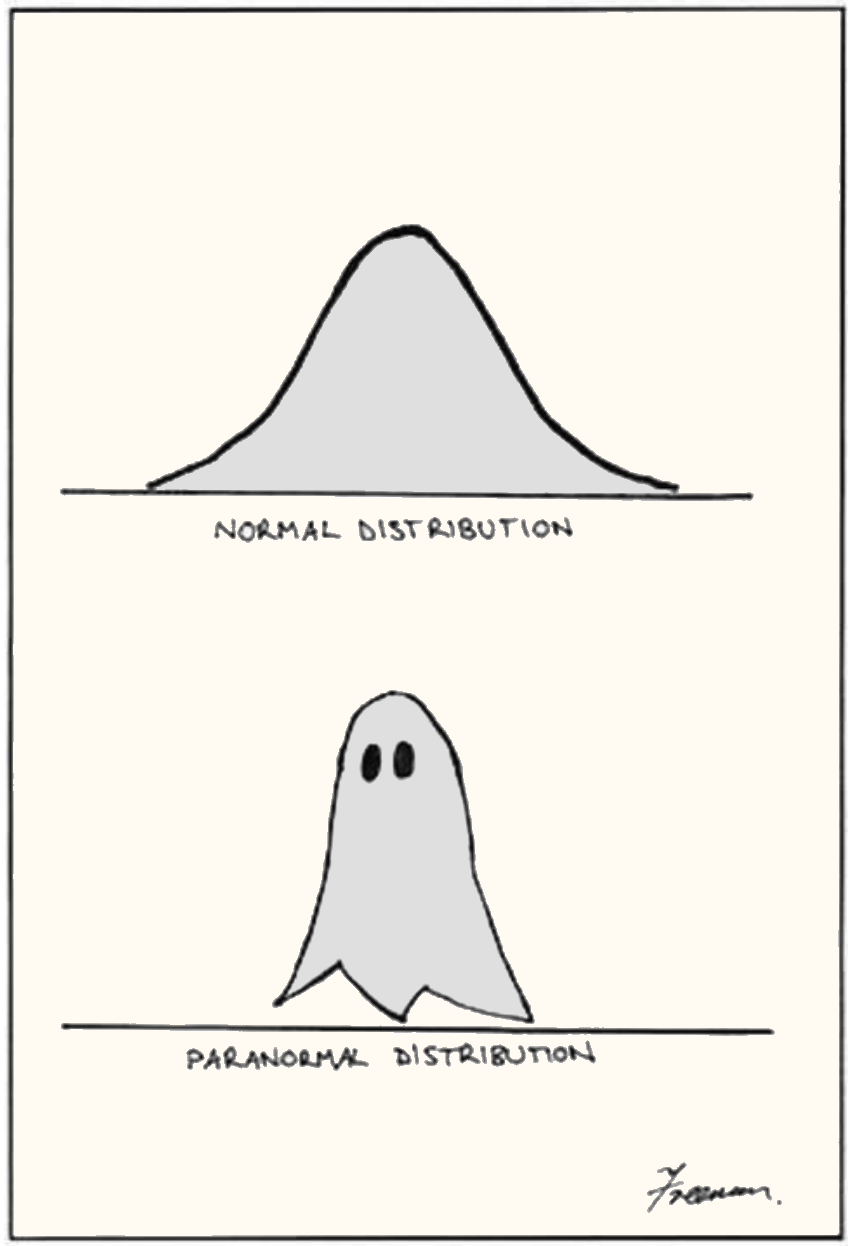
\includegraphics[width=.35\textwidth]{imagenes/imagenes04/T04IM33.png}
	\end{figure}

\newpage
\section{Curiosidades}

	
\begin{myexampleblock}{Aproximaciones entre distintas distribuciones}	
	\begin{figure}[H]
	\centering
	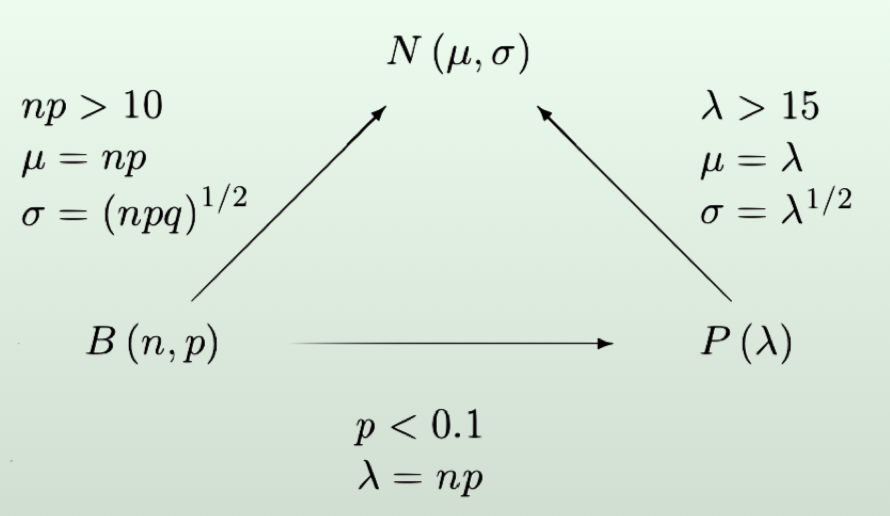
\includegraphics[width=.6\textwidth]{imagenes/imagenes04/T04IM38.png}
	\end{figure}	
\end{myexampleblock}


\vspace{5mm} %************************
\begin{myexampleblock}{El aparato de Galton}

El aparato, tablero  o máquina de Galton es un dispositivo inventado por Francis Galton para demostrar el teorema del límite central, en particular que, con una muestra lo suficientemente grande, la distribución binomial se aproxima a la distribución normal.

\vspace{2mm} La máquina consta de un tablero vertical con varias filas de clavos. Las bolitas caen desde la parte superior, botando aleatoriamente y van depositándose, a medida que caen, en los casilleros de la parte inferior. Formando una superficie de campana.

	\begin{figure}[H]
	\centering
	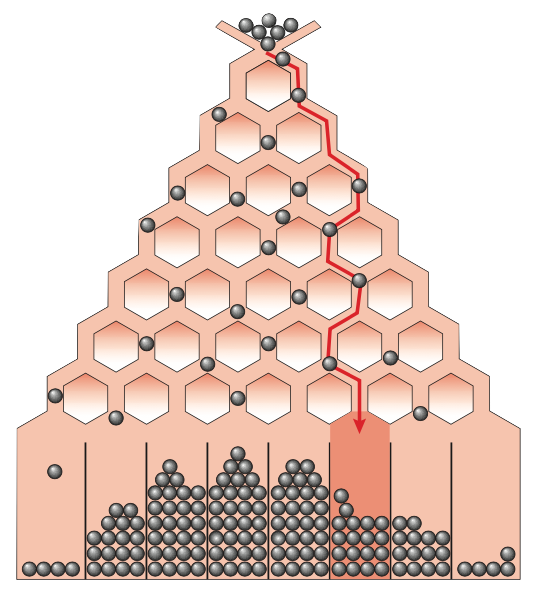
\includegraphics[width=.6\textwidth]{imagenes/imagenes04/T04IM40.png}
	\end{figure}

\vspace{2mm} La x cantidad de bolitas chocarán con el primer clavo teniendo una probabilidad de 1/2 de ir a la izquierda o hacía la derecha, y a medida que continúan va teniendo más caminos a donde ir, es decir más posibilidades para que las bolitas se desvíen. A lo largo de esta estructura, las bolitas toman caminos aleatorios hasta caer en alguno de los canales colocados en la base

\vspace{2mm} Si observamos el recorrido de una bola en el aparato de Galton . En cada bifurcación la bola puede ir a la izquierda con probabilidad p o a la derecha con probabilidad q=1-p. La variable aleatoria que toma valor 0 si cae a la izquierda o 1 si cae a la derecha se llama de Bernouilli y la variable X que da el número de unos al finalizar el experimento (lugares a la derecha) se denomina binomial. Los posibles valores de esta variable dependen del número de pisos que tiene el aparato de Galton.

\vspace{2mm} Si lanzamos una detrás de otra n bolitas al final del recorrido caerán en los distintos canales formando una determinada figura que si repites el experimento varias veces verás que caprichosamente se vuelve a formar casi la misma figura. Es decir estamos obteniendo una aproximación de la distribución de probabilidad. Al final, tendrán mayores probabilidades los canales interiores que los exteriores, formándose la conocida distribución normal.

	\begin{figure}[H]
	\centering
	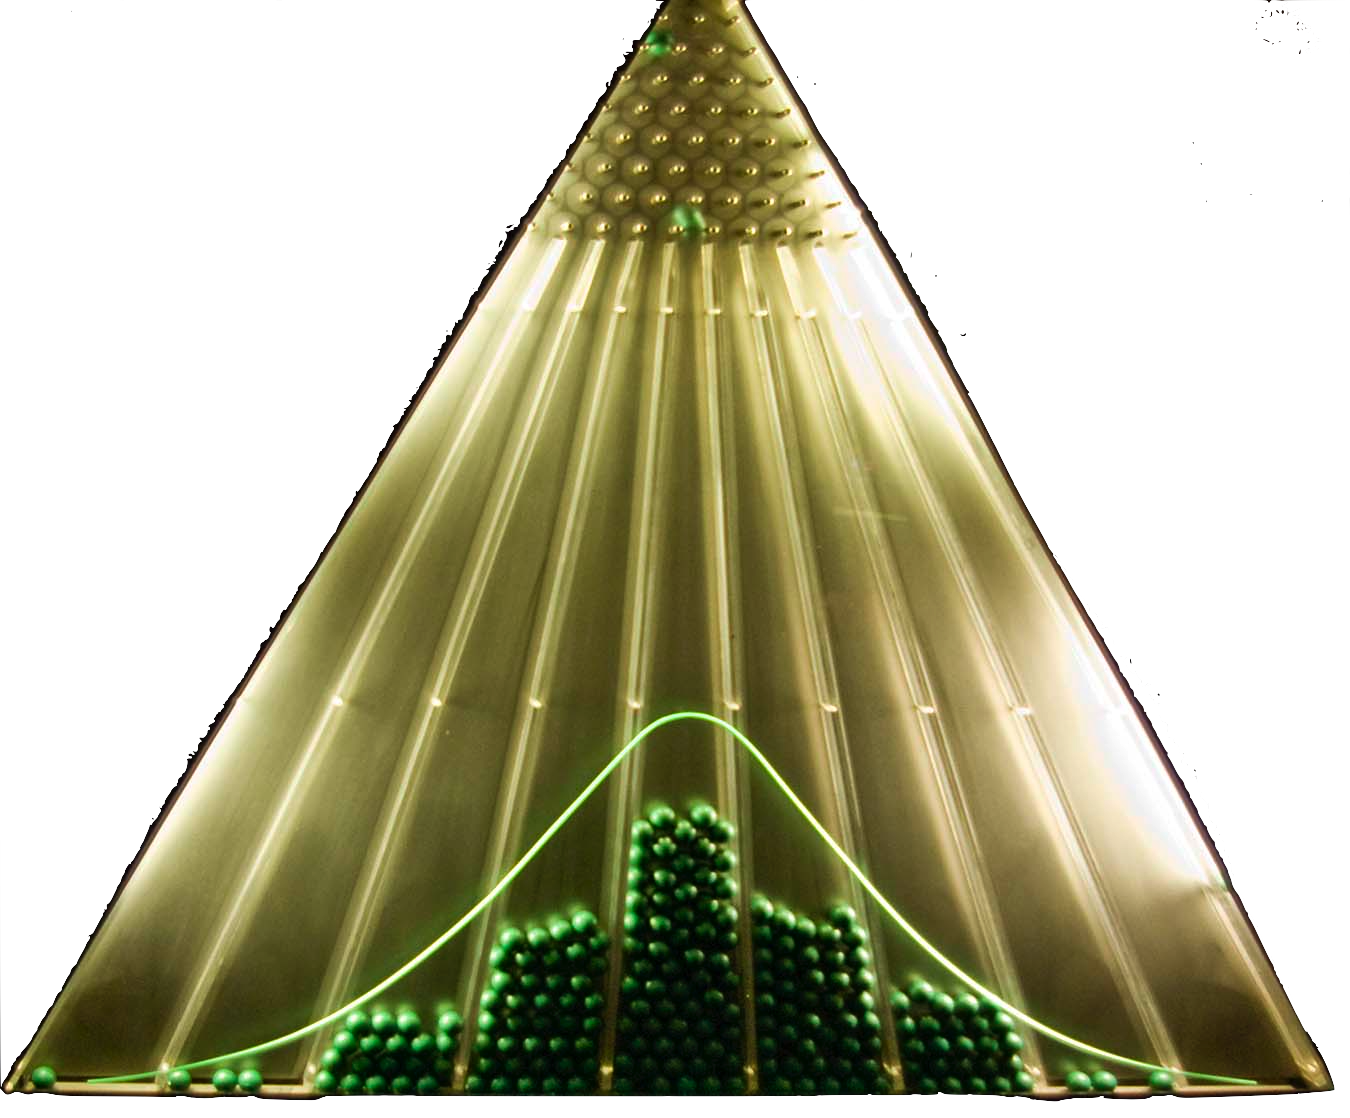
\includegraphics[width=.9\textwidth]{imagenes/imagenes04/T04IM41.png}
	\end{figure}

	
\end{myexampleblock}
	
\vspace{5mm} %************************	
\begin{myexampleblock}
	{$ \divideontimes \  $ Suma de una serie con el valor esperado (sumar derivando)}
	
	\begin{multicols}{2}
		Un señor avanza un paso y lanza una moneda al aire. Si sale cara se detiene y acaba el juego, si sale cruz da otro paso y vuelve a lanzar la moneda. 
		
		La probabilidad de cara es 1/5 y la de cruz 4/5.
	
	\begin{figure}[H]
	\centering
	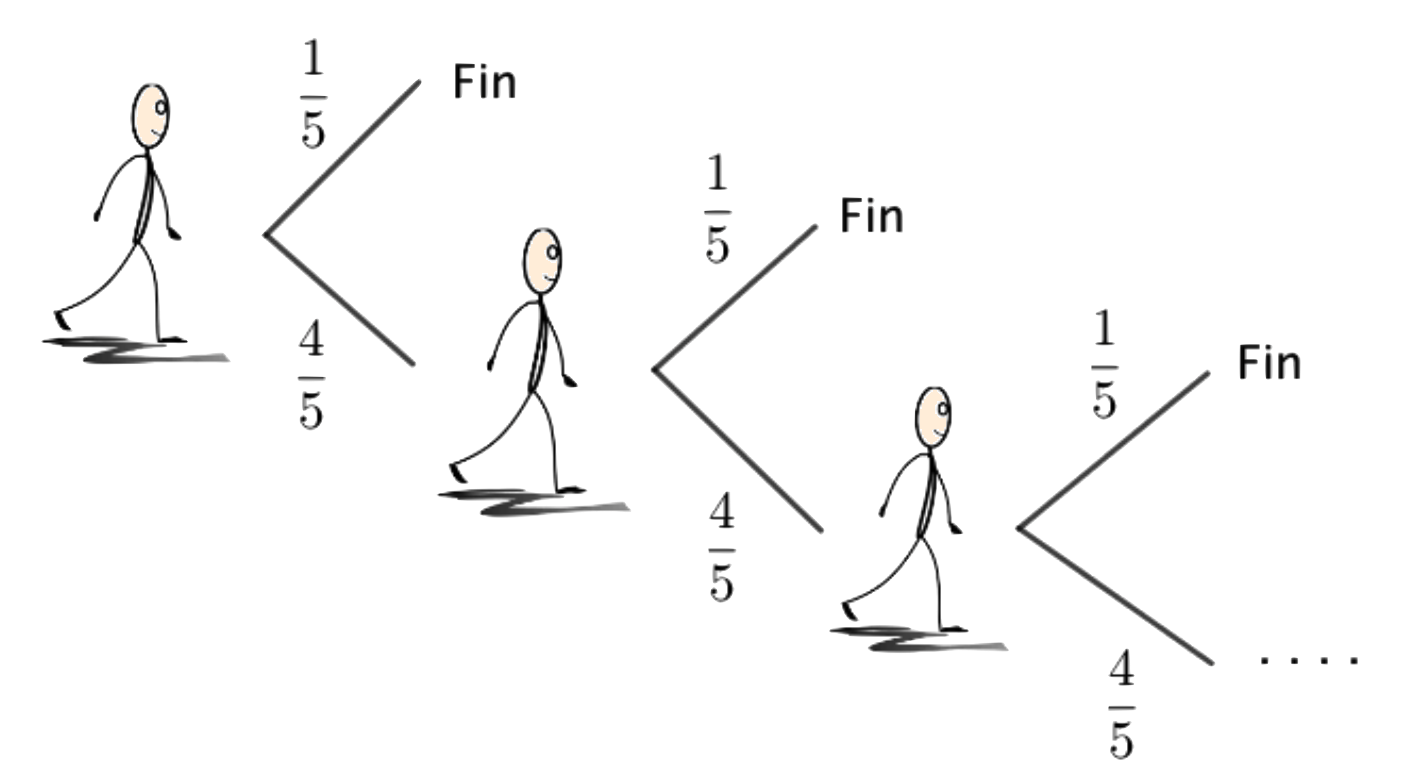
\includegraphics[width=.5\textwidth]{imagenes/imagenes04/T04IM36.png}
	\end{figure}
	\end{multicols}

Evidentemente, la probabilidad de que el Sr. dé n pasos es: 

$p(n)=(4/5)^{n-1}\ (1/5)=4/4\ (4/5)^{n-1}\ (1/5)= 1/4\ (4/5)^n$

Como en 1 de cada 5 ocasiones el juego se detiene, es de sentido común esperar que que el `número de pasos esperado' que dará el Sr. antes de pararse será 5. Calculémoslo:

\vspace{2mm} $E(n) \displaystyle =\sum_{n=1}^\infty n\ p(n)=\sum_{n=1}^{\infty} n \dfrac 1 4 \left( \dfrac 4 5 \right) ^n = \dfrac 1 4 \sum_{n=1}^{\infty} n \left( \dfrac 4 5 \right) ^n$

\vspace{2mm} Si, como hemos dicho, $E(n)=5$, necesariamente, la serie ha de valer $\displaystyle \sum_{n=1}^{\infty} n \left( \dfrac 4 5 \right) ^n=20$

\vspace{2mm}  Un caso más general de serie sería $\ S=\displaystyle \sum_{n=1}^\infty n \ a^n$, con $|a|<1$.

\vspace{2mm} La suma de una Progresión Geométrica de razón menor que uno en valor absoluto es:

\vspace{2mm} $\displaystyle S_{PG}=\sum_{n=1}^\infty a^n=\dfrac 1 {1-a};\ \ |a|<1$; $\qquad S_{PG}=S_{PG}(a)$

\vspace{2mm} Derivando esta expresión, 

\vspace{2mm} --- por una parte: $\ \ \dv{S_{PG}}{a}=\displaystyle \sum_{n=1}^\infty n\ a^{n-1} \ \dfrac a a = \dfrac 1 a \sum_{n=1}^\infty n\ a^n = \dfrac 1 a \ S$

\vspace{2mm} --- por otra parte: $\ \ \dv{S_{PG}}{a}=-\dfrac 1 {(1-a)^2} \ (-1)=\dfrac 1 {(1-a)^2}$

\vspace{2mm} De ambas expresiones: $\ \dfrac 1 {(1-a)^2}=\dfrac 1 a \ S \ \to \ S=\dfrac{1}{(1-a)^2}$

\vspace{2mm} En nuestro caso, para $a=4/5 \ \to \ S=20$ !!!!!
	
\end{myexampleblock}


%\newpage
%\includepdf[pages=-]{imagenes/imagenes04/resumen-distrib-prob.pdf}

\newpage


$\quad$

$\quad$

$\quad$

\begin{myblock}{RESUMEN: Distribuciones de probabilidad}

$\quad$

\vspace{5mm} $\triangleright \ $ Distribución binomial.
	
	$$B(n,p) 
	\qquad : \qquad \qquad
	p(X_k)=\mqty(n\\k) \ p^k\ (1-p)^{n-k}$$
	
	\vspace{5mm} $\triangleright \ $ Distribución normal.
	
	\begin{figure}[H]
	\centering
	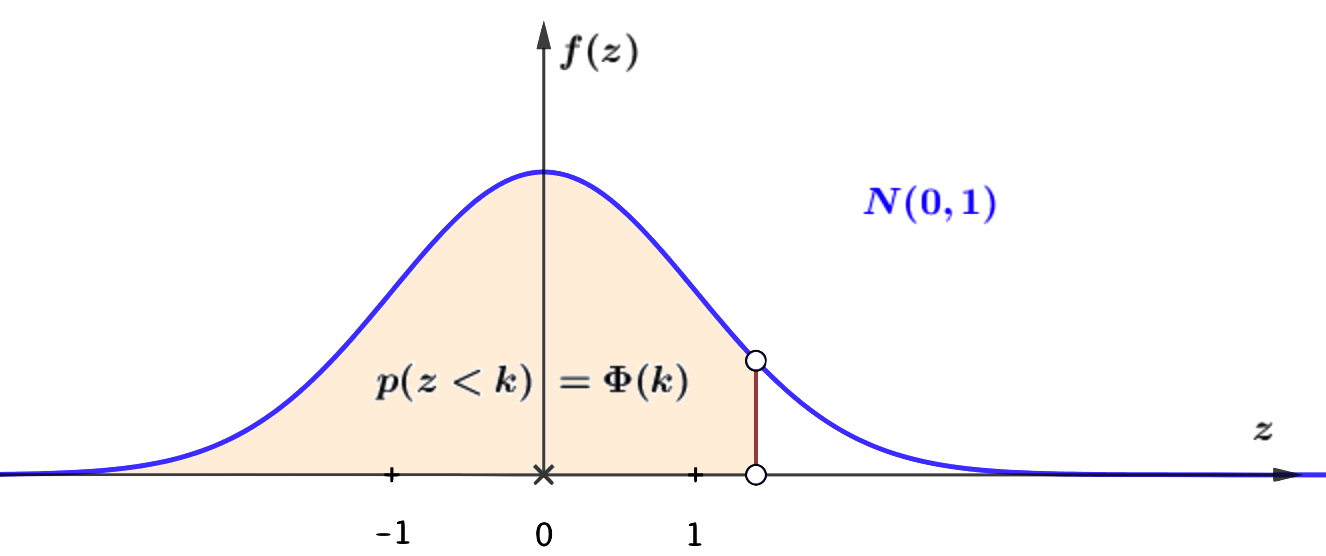
\includegraphics[width=.75\textwidth]{imagenes/imagenes04/T04IM43.png}
	\end{figure}
	
	$$N(\mu,\sigma) \ \to \ \text{ TIPIFICACIÓN } \ x\in N(\mu,\sigma) \ \to \ \boldsymbol{ z=\dfrac{x-\mu}{\sigma} } \in N(0,1)$$

\vspace{5mm} $\triangleright \ $ La binomial se aproxima a la normal.
	
	$$\begin{matrix}
n\ge 30\ \ \ 	\wedge \ \ \ np\ge 5 \ \ \ \wedge \ \ \ n(1-p)\ge 5 
\\ \\
B (np) \ \approx \ N \left( \ \mu=np \ , \ \sigma=\sqrt{np(1-p} \ \right)
\end{matrix}$$



$$x\in B(n,p) 
\quad
\underrightarrow{\text{\footnotesize{\textcolor{blue}{Corrección por continuidad}}}}
\quad 
x'\in N(\mu,\sigma) 
\quad
\underrightarrow{\text{\footnotesize{Tipificación}}}
\quad
z\in N(0,1)
$$

$\quad$

\end{myblock}









